\appendix

\renewcommand{\thechapter}{A}
\refstepcounter{chapter}
\makeatletter
\renewcommand{\theequation}{\thechapter.\@arabic\c@equation}
\makeatother
\chapter*{\LARGE Appendix A \\\tiny\vspace{-0.4\baselineskip} \LARGE Lab to CMS transformation}
\label{app_lab_cms_trans}
\addcontentsline{toc}{chapter}{Appendix A: Lab to CMS transformation}



Here the procedure of the Lab to CMS transformation for an electroproduction experiment off the proton at rest (bottom left illustration in Fig.~\ref{fig:lab_to_CMS}) is described~\cite{Fed_an_note:2017}. In this case the CMS axis orientation is different for each reaction event and is specified by the direction of the scattered electron. The transformation from Lab to CMS includes the following steps\footnote[1]{In all derivations the energy is assumed to be the last component of the four-momentum and the four-momentum to be a row vector.}:%\vspace{-1em}

\begin{enumerate}
\item The $xy$-plane of the Lab system is rotated around the $z$-axis (given by the incoming electron direction) to make the $x$-axis lying in the electron scattering plane (see Fig.~\ref{fig:cr_sec_el_angles}). This rotation transforms the four-momentum as $P' = P \cdot R_1(\varphi_{e'})$, with 
\begin{equation}
R_{1}(\varphi_{e'}) = \begin{pmatrix}
 \cos\varphi_{e'}& -\sin\varphi_{e'} & 0 &0 \\ 
 \sin\varphi_{e'}& \cos\varphi_{e'} &  0& 0\\ 
0 & 0 & 1 &0 \\ 
 0&  0&  0&1 
\end{pmatrix},
\end{equation}
where $\varphi_{e'}$ is the azimuthal angle of the scattered electron.
\begin{figure}[htp]
\begin{center}
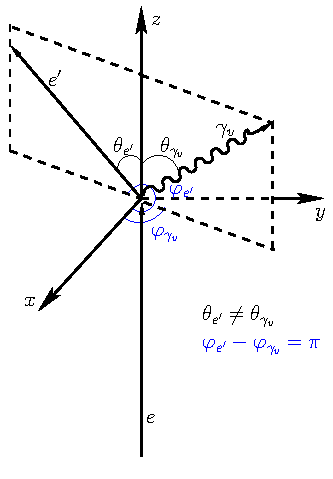
\includegraphics[width=5.8cm]{pictures/appendix/electron_angles.pdf}
\caption{\small Virtual photon and scattered electron angles $\theta$ and $\varphi$ in the Lab frame for the proton at rest experiment.} \label{fig:cr_sec_el_angles}
\end{center}
\end{figure}

%\vspace{-1em}
After this rotation $\varphi_{e'} = 0$, while $\varphi_{\gamma_v} = \pi$ with respect to the intermediate reference frame.

\item The Lab system is then rotated to align the $z$-axis with the virtual photon direction. The four-momentum transformation for this rotation is given by $P'' = P' \cdot R_2 (\theta_{\gamma_{v}})$, with 
\begin{equation}
R_{2}(\theta_{\gamma_{v}})=\begin{pmatrix}
\cos\theta_{\gamma_{v}} &0  &-\sin\theta_{\gamma_{v}}  &0 \\ 
 0& 1 & 0 &0 \\ 
 \sin\theta_{\gamma_{v}} &0  &\cos\theta_{\gamma_{v}}  & 0\\ 
0 &0  & 0 &1 
\end{pmatrix},
\end{equation}
where $\theta_{\gamma_v}$ is the polar angle of the virtual photon\footnote[2]{Using embedded ROOT functions, both rotations can be coded using the unit vectors TVector3~$uz$~=~P4\_gamma.Vect().Unit() and 
 TVector3~$ux$~=~(P4\_EL.Vect().Cross(P4\_ELP.Vect())).Unit(), where P4\_gamma, P4\_EL, and P4\_ELP are the four-momenta of the virtual photon, initial and final electrons, respectively. 
 The axis vector $ux$ needs to be rotated according to $ux$.Rotate(3.*M\_PI/2,$uz$).
Finally the rotation is defined as rot.SetZAxis($uz$,$ux$).Invert() and needs to be applied to the four-momentum (P4) of each particle:
 P4.Transform(rot).}.

\item Finally, a boost into the CM frame of the {\em virtual photon -- initial proton} system is performed. It is given by the formula $P''' = P'' \cdot R_3(\beta)$, with 
\begin{equation}
R_{3}(\beta) = \begin{pmatrix}
1 &0  &0  &0 \\ 
0 &1  &0  &0 \\ 
 0&  0& \gamma  &-\gamma \beta  \\ 
 0&  0& -\gamma \beta  & \gamma 
\end{pmatrix}, \, \, \, \beta =\frac{|\overrightarrow{q}|}{E_{\gamma }+m_{proton}}=\frac{\sqrt{E^{2}_{\gamma }+Q^{2}}}{E_{\gamma }+m_{proton}}, \, \, \,\,  \gamma =\frac{1}{\sqrt{1-\beta ^{2}}},
\end{equation}
where $|\overrightarrow{q}|$ is the magnitude of the three-vector of the virtual photon and $\beta$ the magnitude and $z$-component of the three-vector\footnote[3]{Note: if you use the ROOT function .Boost, you should change the sign of the $z$-component of $\beta$-vector as .Boost(0,0,-$\beta$).} $\overrightarrow{\beta}=(0,0,\beta)$.
\end{enumerate}

%================================================

\renewcommand{\thechapter}{B}
 \refstepcounter{chapter}
    \makeatletter
   \renewcommand{\theequation}{\thechapter.\@arabic\c@equation}
    \makeatother
\chapter*{Appendix B \\\tiny\vspace{-0.4\baselineskip} \LARGE The reaction phase-space}
\label{app_ph_space}
\addcontentsline{toc}{chapter}{Appendix B: The reaction phase-space}



The phase-space of the reaction $ep \rightarrow e'p'\pi^{+}\pi^{-}$ is determined by seven kinematic variables, i.e. $W$, $Q^{2}$, $M_{h_{1}h_{2}}$, $M_{h_{2}h_{3}}$, $\theta_{h_{1}}$, $\varphi_{h_{1}}$, and $\alpha_{h_{1}}$ (see Sect.~\ref{Sect:kin_var} for details). The kinematic coverage for various variables has the following specificities.\vspace{-0.2em} 
\begin{itemize}
\item In the $W$ and $Q^{2}$ variables it depends on the electron beam energy and experimental conditions and is fixed for a particular experiment. \vspace{-0.3em}
\item The angular variables $\theta_{h_{1}}$, $\varphi_{h1}$, and $\alpha_{h1}$ vary in the fixed limits of $[0,~\pi]$, $[0,~2\pi]$, and $[0,~2\pi]$, respectively.\vspace{-0.3em}
\item In the invariant masses $M_{h_{1}h_{2}}$ and $M_{h_{2}h_{3}}$ the coverage depends on $W$ and broadens as $W$ grows.\vspace{-0.2em}
\end{itemize}
\vspace{-1em}
\begin{figure}[htp]
\begin{center}
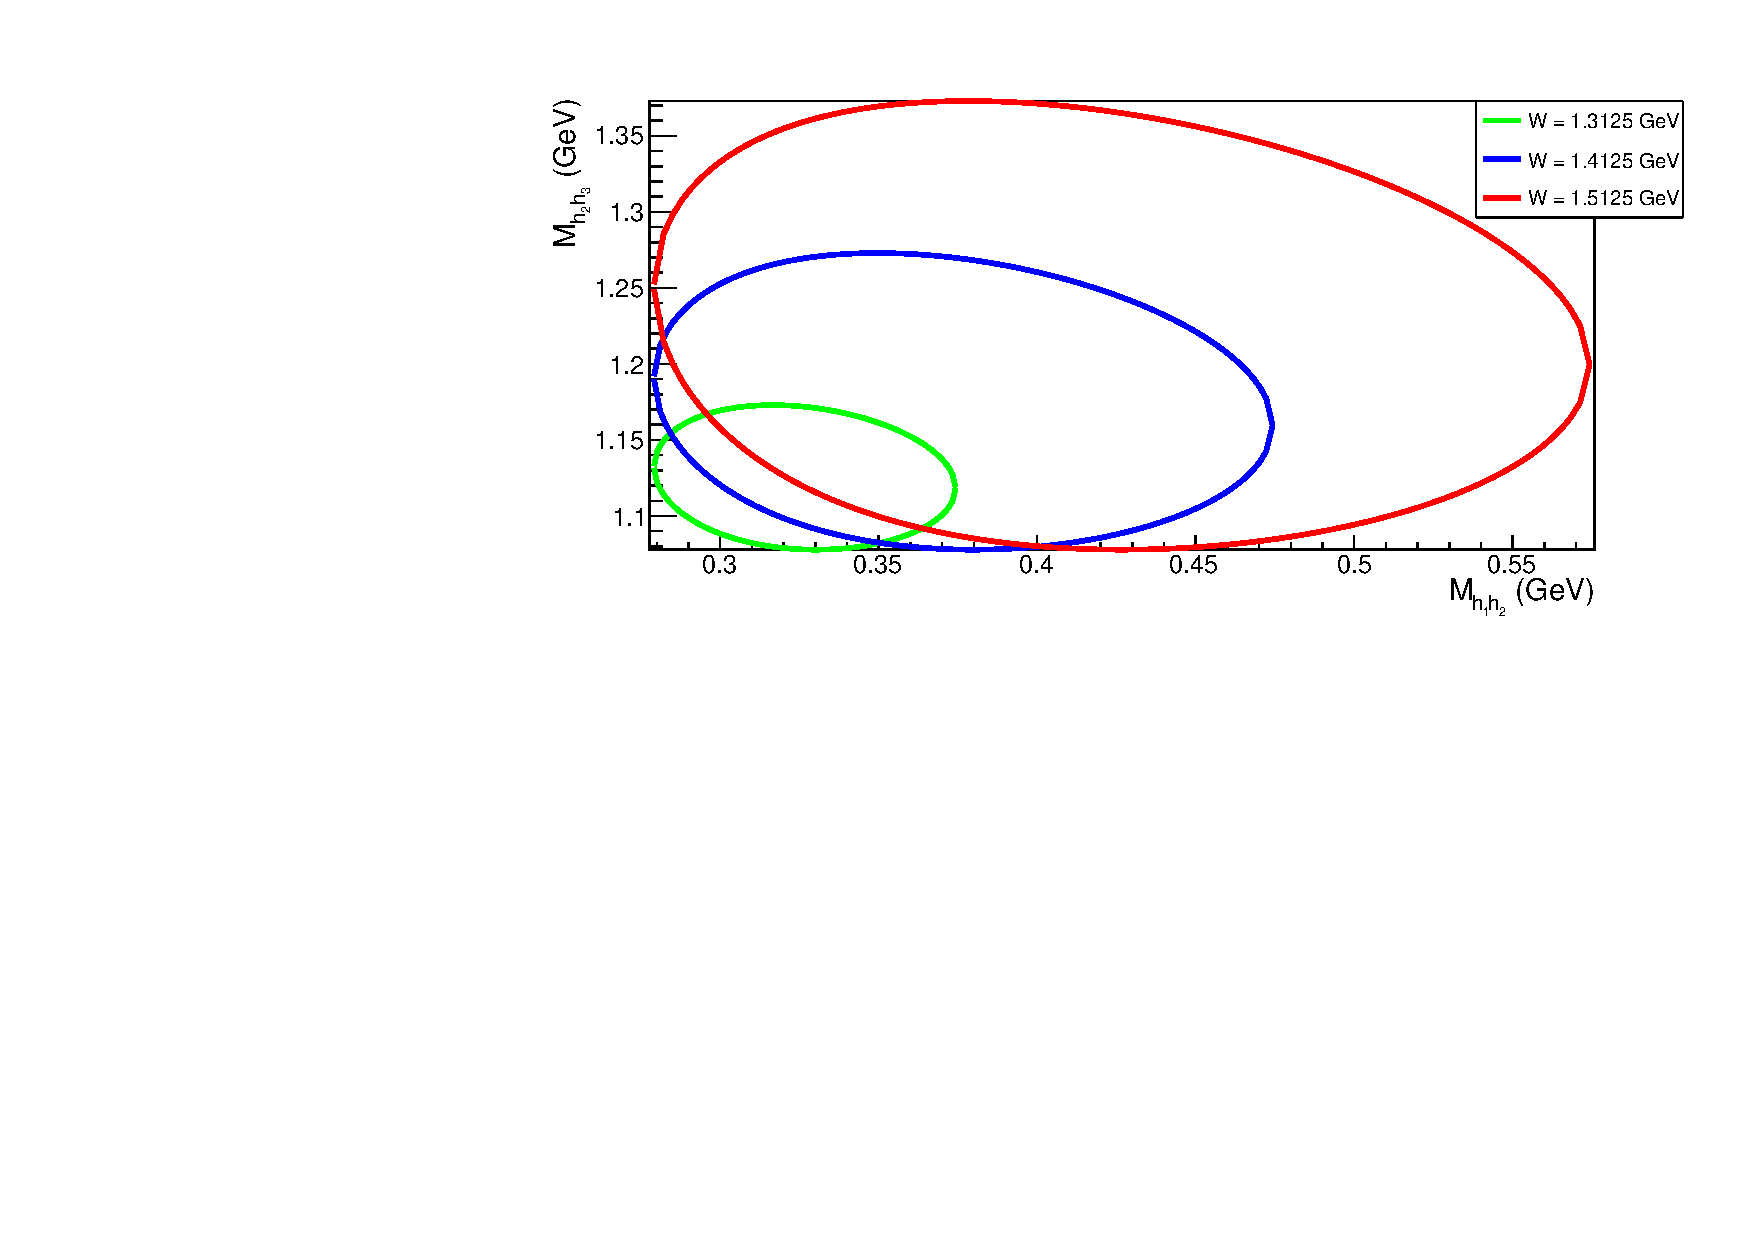
\includegraphics[width=13cm]{pictures/appendix/dalitz_plots_boundaries.pdf}
\caption{\small Boundary of the $M_{h_{2}h_{3}}$ versus $M_{h_{1}h_{2}}$ distribution for several distinct values of $W$ specified in the plot.} \label{fig:dalitz}
\end{center}
\end{figure}

The shape of the reaction phase-space in the invariant masses is determined by the condition $B(M_{h_{1}h_{2}}^{2}, M_{h_{2}h_{3}}^{2}, W^{2}, m_{h_{2}}^{2}, m_{h_{1}}^{2}, m_{h_{3}}^{2}) = 0$, where $B(x, y, z, u, v, w)$ is the Byckling function~\cite{Byckling:1971vca} given by 
\begin{equation}
\begin{split}
B(x,y,z,u,v,w) = &x^{2}y+xy^{2}+z^{2}u+zu^{2}+v^{2}w+vw^{2}+ \\   
&xzw+xuv+yzv+yuw- xy(z+u+v+w)- \\ 
&zu(x+y+v+w)-vw(x+y+z+u).
\label{eq:byckling}
\end{split}
\end{equation}

Figure~\ref{fig:dalitz} shows the boundary of the $M_{h_{2}h_{3}}$ versus $M_{h_{1}h_{2}}$ distribution for several values of $W$ specified in the plot and visually demonstrates the effect  of the phase-space broadening with the increase of $W$.


%============================================


\renewcommand{\thechapter}{C}
 \refstepcounter{chapter}
    \makeatletter
   \renewcommand{\theequation}{\thechapter.\@arabic\c@equation}
    \makeatother
\chapter*{\LARGE Appendix C \\\tiny\vspace{-0.4\baselineskip} \LARGE Uncertainties for indirect measurements}
\label{app_uncert}
\addcontentsline{toc}{chapter}{Appendix C: Uncertainties for indirect measurements}



Some useful examples of the error propagation for indirect measurements are described here. In these examples one assumes that $a>0$, $b>0$, and $c>0$.



\begin{itemize}

\item If independent variables $x_{1}$ and $x_{2}$ have absolute uncertainties $\Delta x_{1}$ and $\Delta x_{2}$, respectively, then the absolute uncertainty of the variable $y=c(\frac{x_{1}}{a} - \frac{x_{2}}{b})$ is
\begin{equation}
\begin{aligned}
\Delta y = c\sqrt{\left (\frac{ \Delta x_{1}}{a} \right )^{2} + \left (\frac{ \Delta x_{2}}{b} \right )^{2}}.
\label{eq:err_subtr}
\end{aligned}
\end{equation}


\item If the variable $x$ has an absolute uncertainty $\Delta x$, then the absolute uncertainty of the variable $y=\frac{a}{x}$ is
\begin{equation}
\begin{aligned}
\Delta y = \frac{a}{x^{2}}\cdot \Delta x = y\cdot \frac{\Delta x}{x}.
\label{eq:err_frac}
\end{aligned}
\end{equation}


\item If the variable $x$ has an absolute uncertainty $\Delta x$, then the absolute uncertainty of the variable $y=\frac{a\cdot x +b}{c}$ is
\begin{equation}
\begin{aligned}
\Delta y = \frac{a\cdot \Delta x}{c}.
\label{eq:err_prod}
\end{aligned}
\end{equation}



\item If there is a set of measurements $x_{1}$, $x_{2}$, ..., $x_{n}$ with the arithmetic mean $\overline{x}$, then the absolute standard error of the arithmetic mean is
\begin{equation}
\begin{aligned}
\Delta \overline{x} = \sqrt{\frac{\sum\limits_{i=1}^{n} (x_{i}-\overline{x})^{2}}{n\cdot(n-1)}}.
\label{eq:err_arith_mean}
\end{aligned}
\end{equation}

\end{itemize}

%============================================

\renewcommand{\thechapter}{D}
 \refstepcounter{chapter}
    \makeatletter
   \renewcommand{\theequation}{\thechapter.\@arabic\c@equation}
    \makeatother
\chapter*{Appendix D \\\tiny\vspace{-0.4\baselineskip} \LARGE Measured single-differential cross sections}
\label{app_cr_sect}
\addcontentsline{toc}{chapter}{Appendix D: Measured single-differential cross sections }


This Appendix contains the full set of single-differential cross sections measured in the current analysis. The cross sections are reported with the uncertainty $\delta_{\text{stat,mod}}^{\text{tot}}$ shown by the error bars (see Sect.~\ref{Sect:uncert_resume}). The central point of the corresponding $W$ and $Q^{2}$ bin is specified in the title of each figure together with the value of the relative integral systematic uncertainty $\varepsilon_{\text{sys}}$ that can be propagated as a global factor to the corresponding single-differential cross sections (see Sect.~\ref{Sect:sys_uncert}).

Note that the invariant mass distributions are shown in the range from $M_{lower}$ to $M_{upper}$, both given by Eq.~\eqref{eq:inv_mass_boundary} with the latter calculated using the central value of the $W$ bin. One, therefore, should take into consideration that, for each invariant mass, the cross section is equal to zero on both sides of the range. Also note that the invariant mass distributions contain one bin less than specified in Tab.~\ref{tab:summary_bins}, since the cross section in the last mass bins is not reported. This happens due to the special arrangement of thhe mass bins used in the analysis, which forces the last bin to be situated out of the specified range (see Sect.~\ref{Sect:binning} for details).  


It is also noteworthy that $\alpha$ angular distributions of the double-pion cross sections should be symmetrical with respect to $\alpha = 180^{\rm o}$, when integrated over $\varphi$. However, the experimentally measured $\alpha$ distributions acquire some asymmetry. To judge more quantitatively the asymmetry degree, the average asymmetry factor was estimated for each extracted $\alpha$ distribution as\newpage
\begin{equation}
\begin{aligned}
\textrm{asym} = \frac{1}{\textrm{int} [ n/2]} \sum_{\substack{i = 1}}^{\substack{\textrm{int}[ n/2]}} \left | 1 - \frac{2\sigma_{i}}{\sigma_{i}+\sigma_{n-i}}\right |,
\label{eq:asym}
\end{aligned}
\end{equation}
where $n$ is the number of bins in the distribution and $\sigma_{i}$ the cross section value in the bin $i$.

The average asymmetry factor estimated by Eq.~\eqref{eq:asym} is specified in the plots above each $\alpha$ distribution to facilitate visual judgement of the distribution shape and its inherent systematic inaccuracy.

\begin{figure}[htp]
\begin{center}
\frame{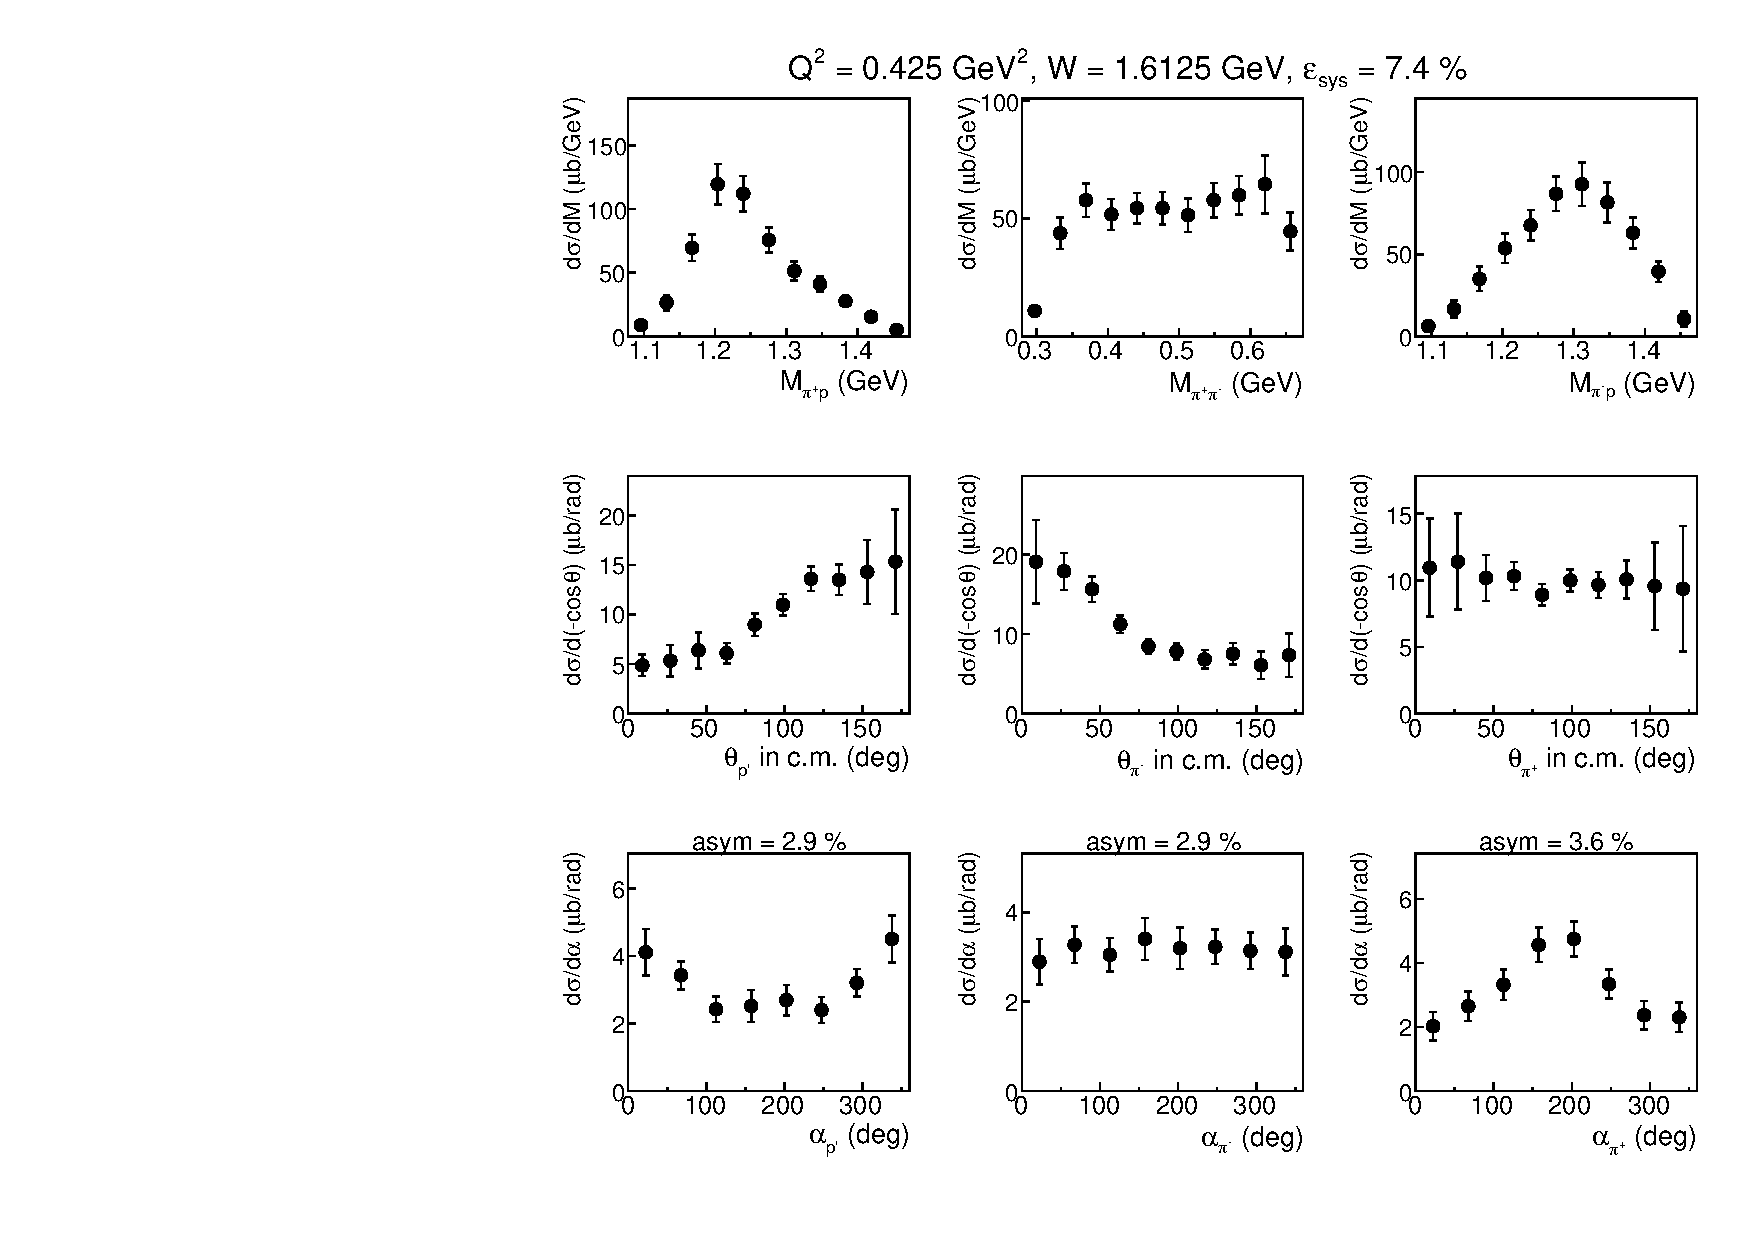
\includegraphics[width=0.495\textwidth]{pictures/appendix/1diff_distr/Q2_425/w_16125.pdf}}
\frame{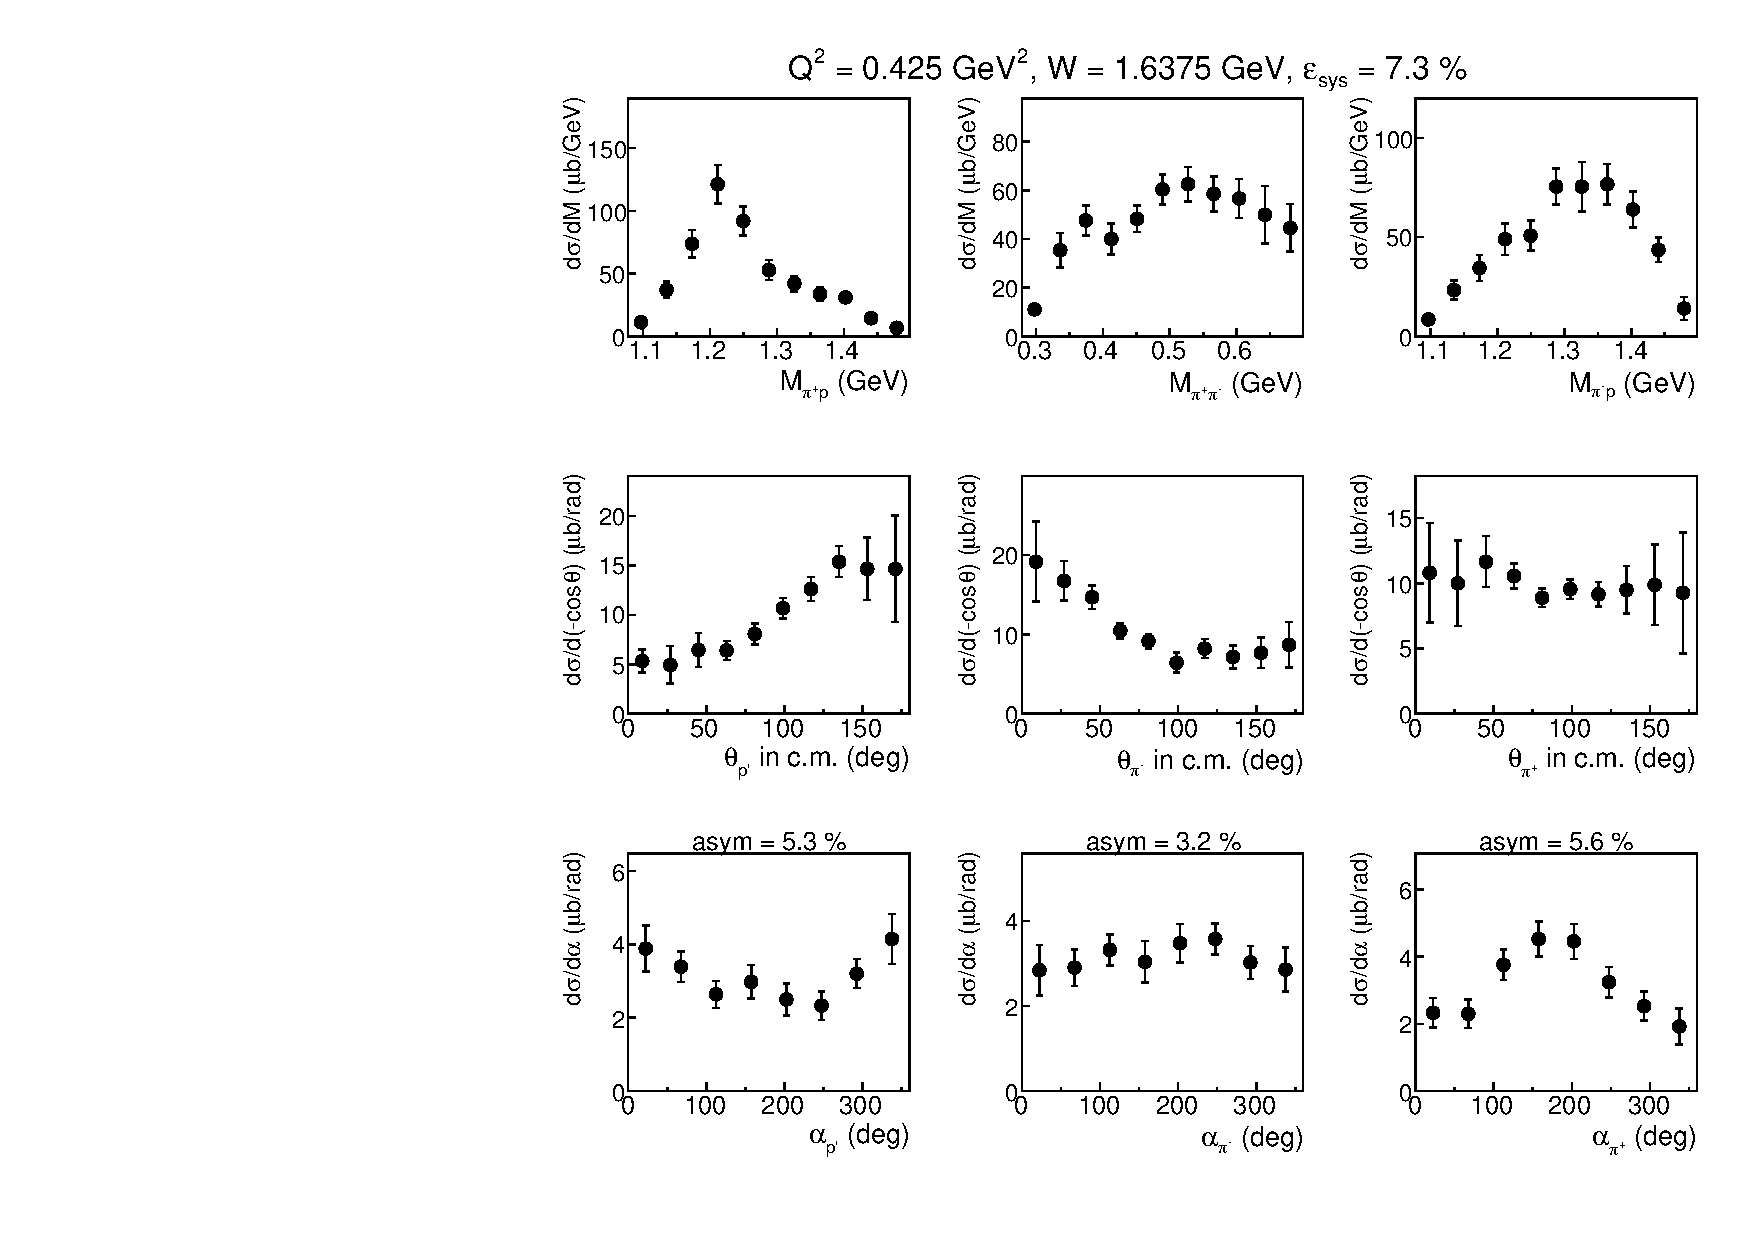
\includegraphics[width=0.495\textwidth]{pictures/appendix/1diff_distr/Q2_425/w_16375.pdf}}
\frame{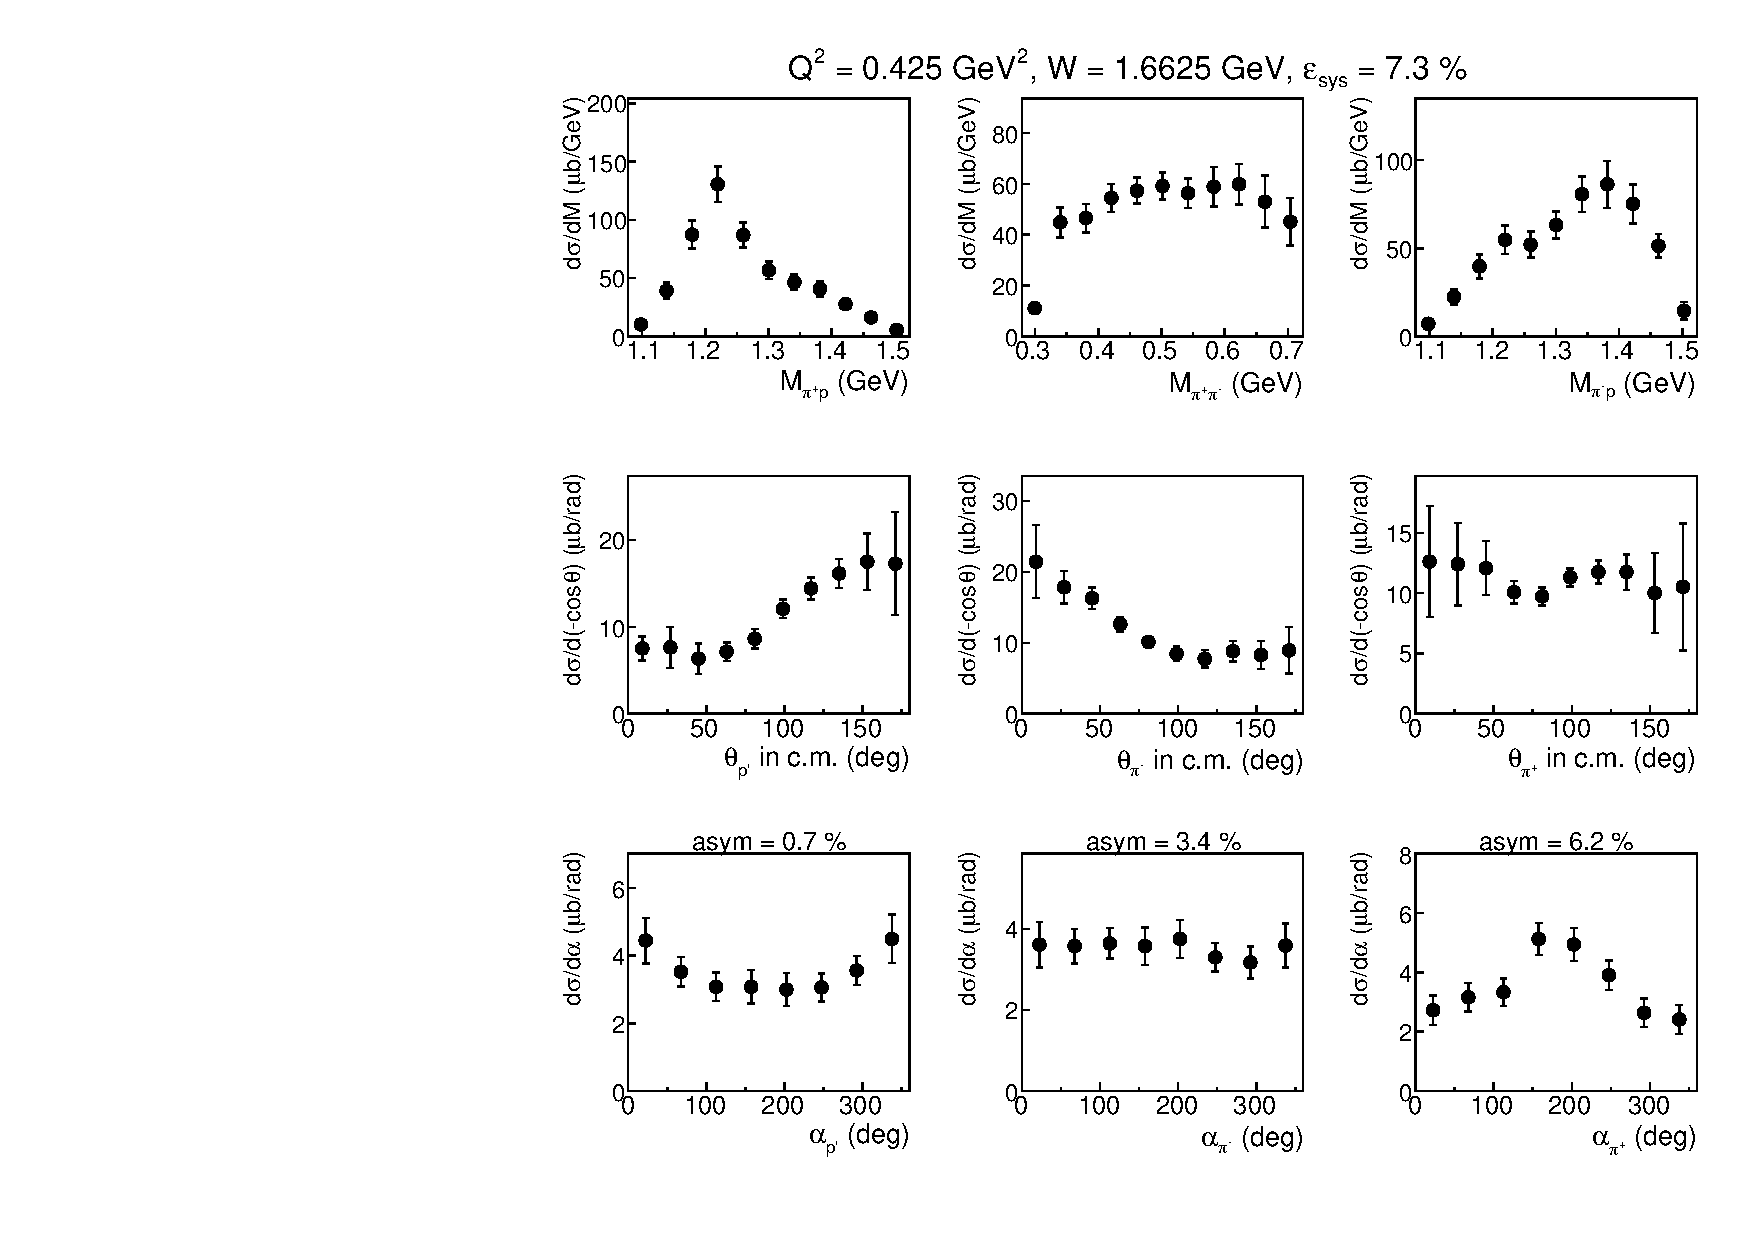
\includegraphics[width=0.495\textwidth]{pictures/appendix/1diff_distr/Q2_425/w_16625.pdf}}
\frame{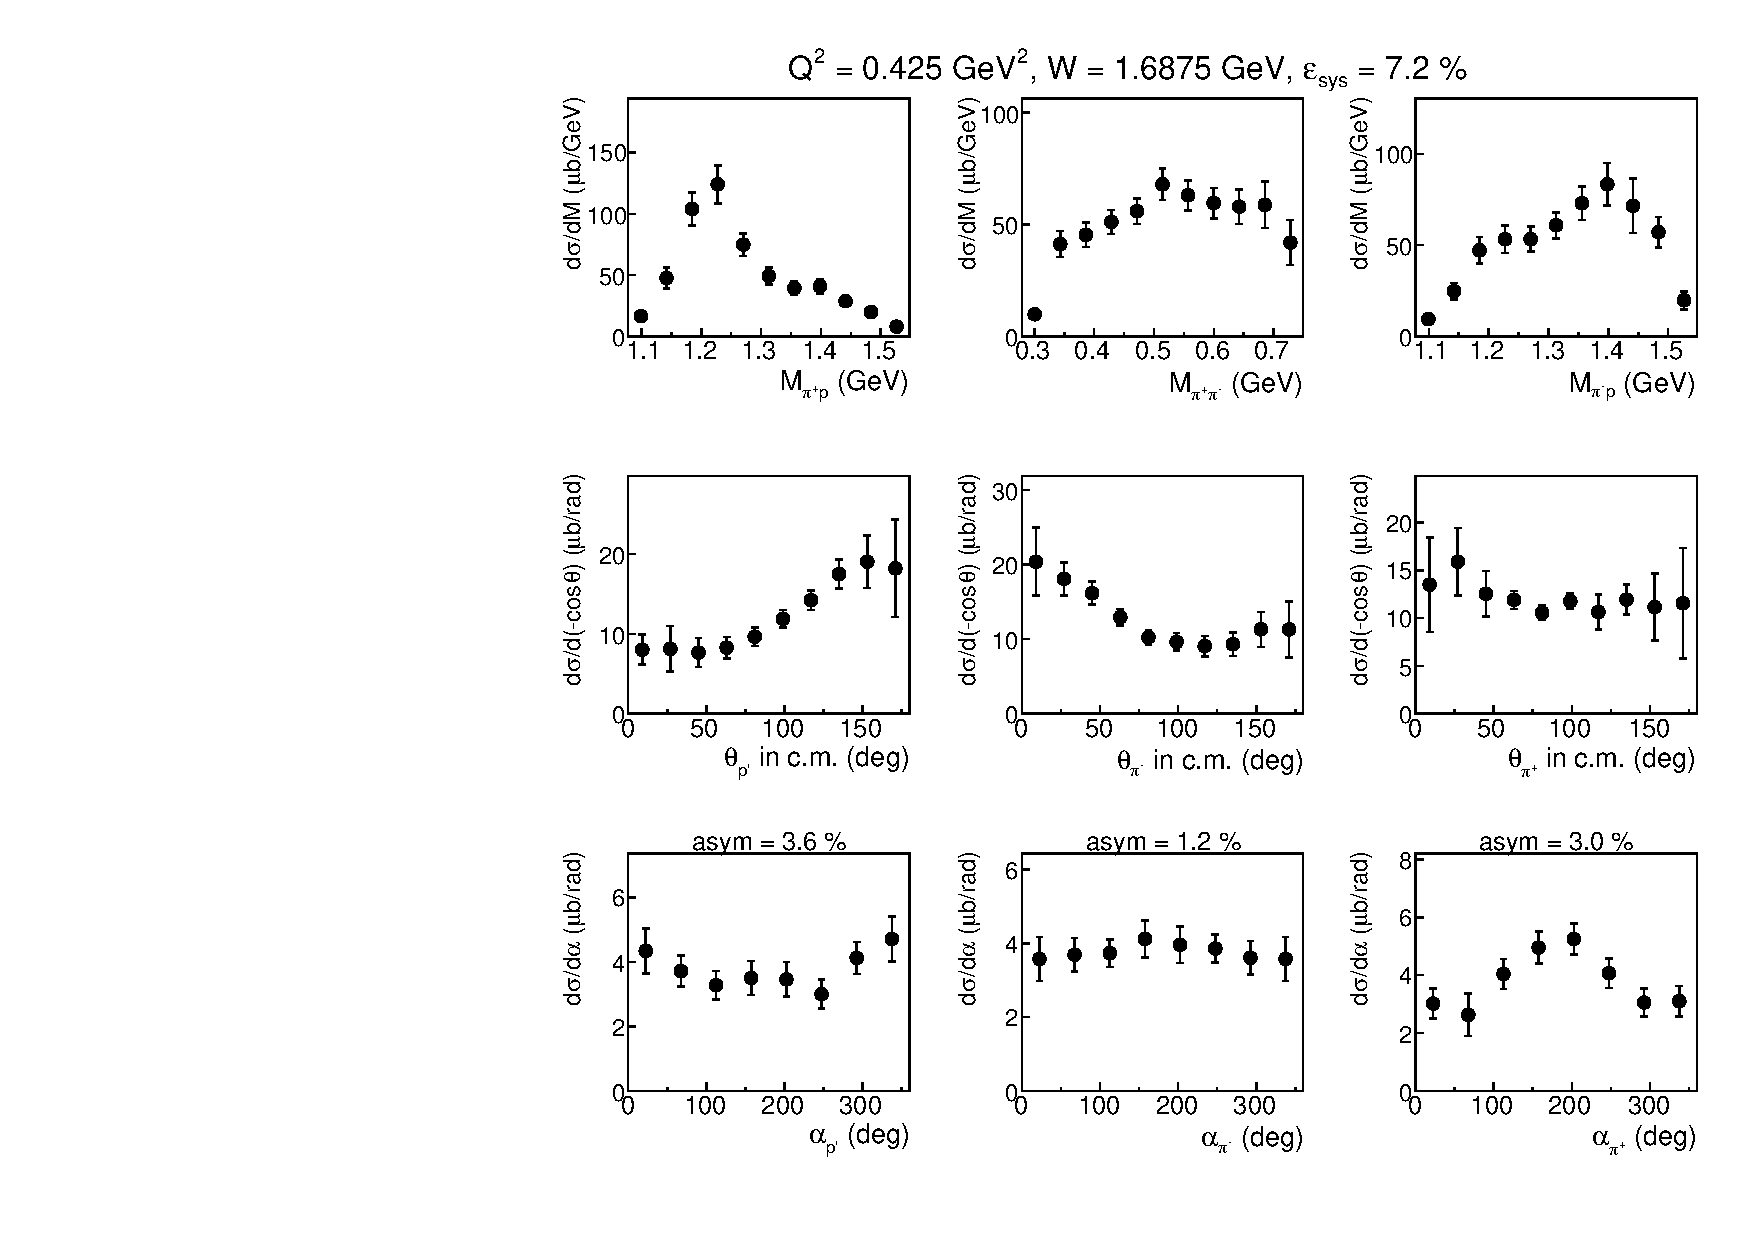
\includegraphics[width=0.495\textwidth]{pictures/appendix/1diff_distr/Q2_425/w_16875.pdf}}
\caption{\small Measured single-differential cross sections.} \label{fig:appx_1}
\end{center}
\end{figure}

\clearpage
\begin{figure}[htp]
\begin{center}
\frame{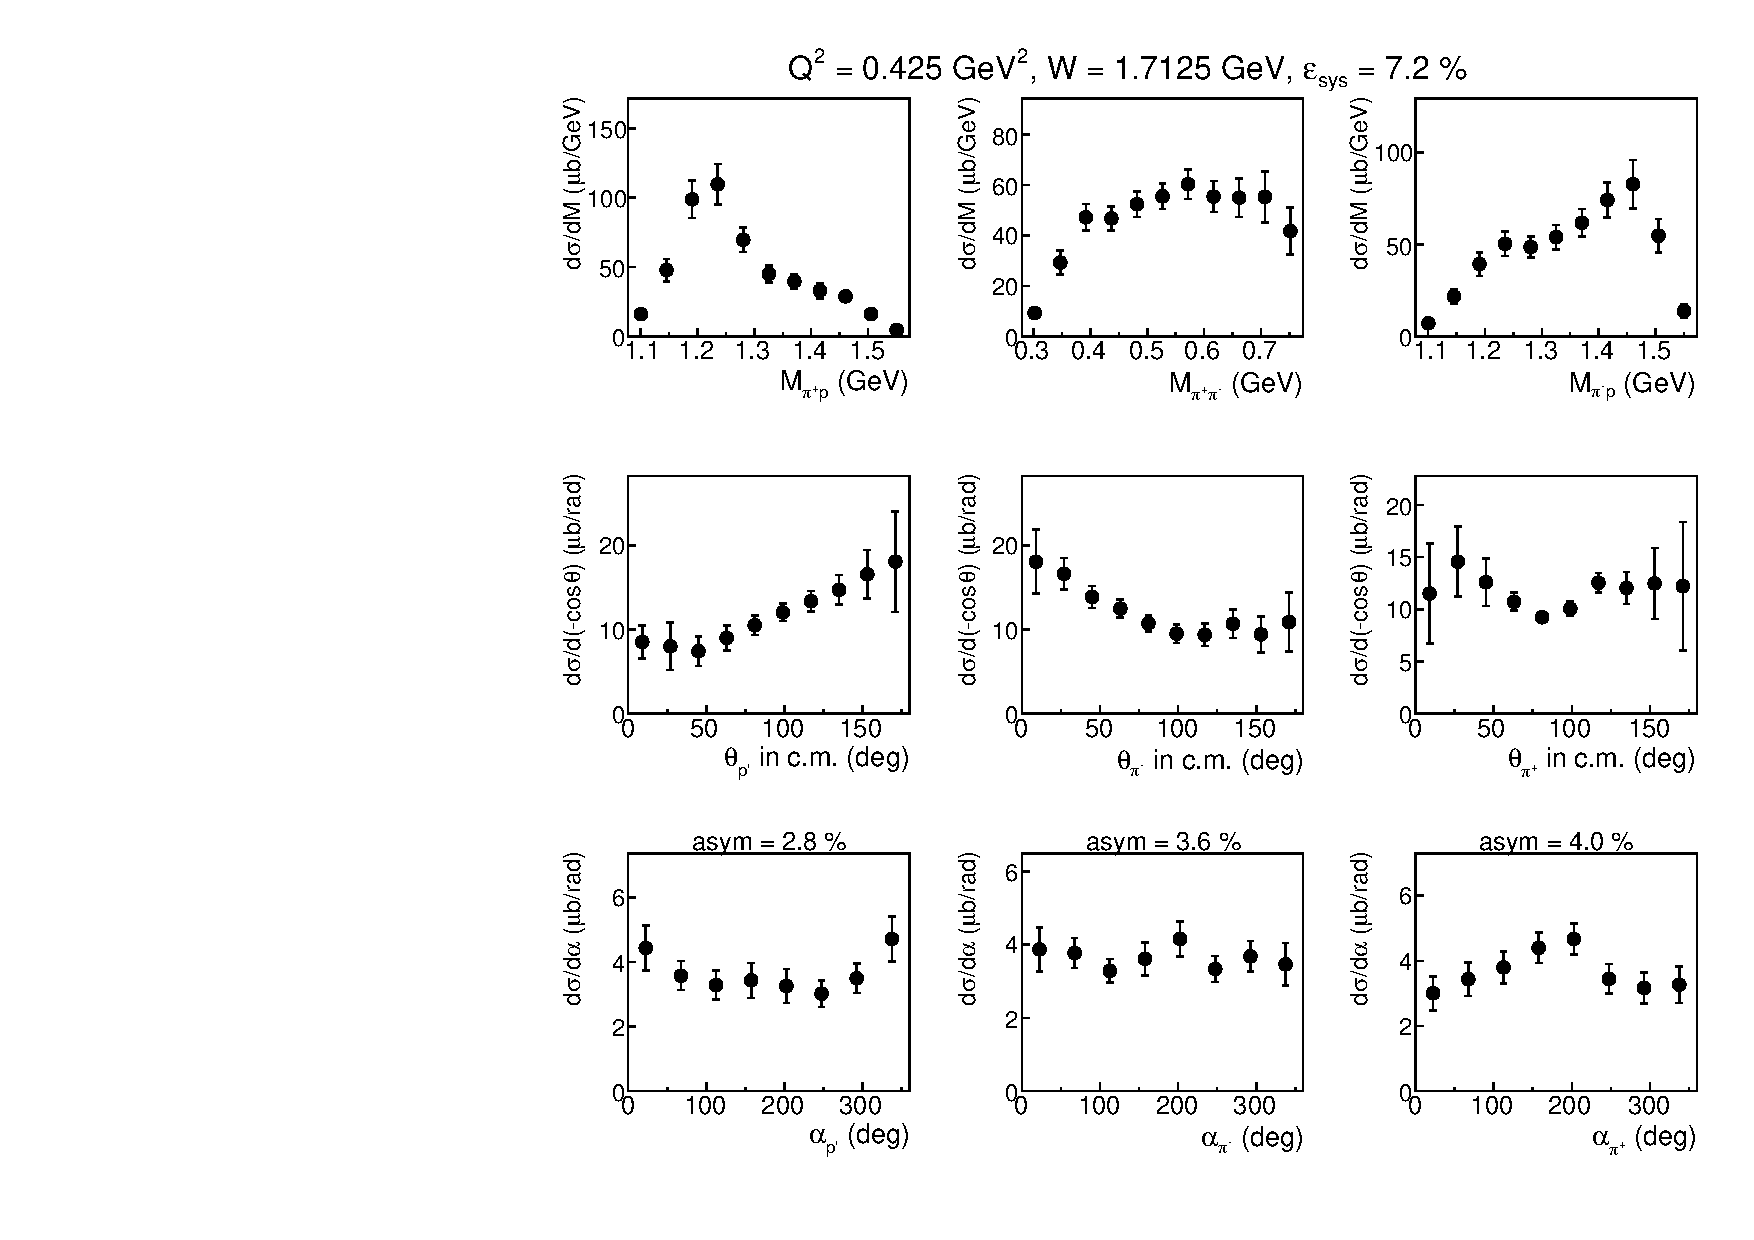
\includegraphics[width=0.495\textwidth]{pictures/appendix/1diff_distr/Q2_425/w_17125.pdf}}
\frame{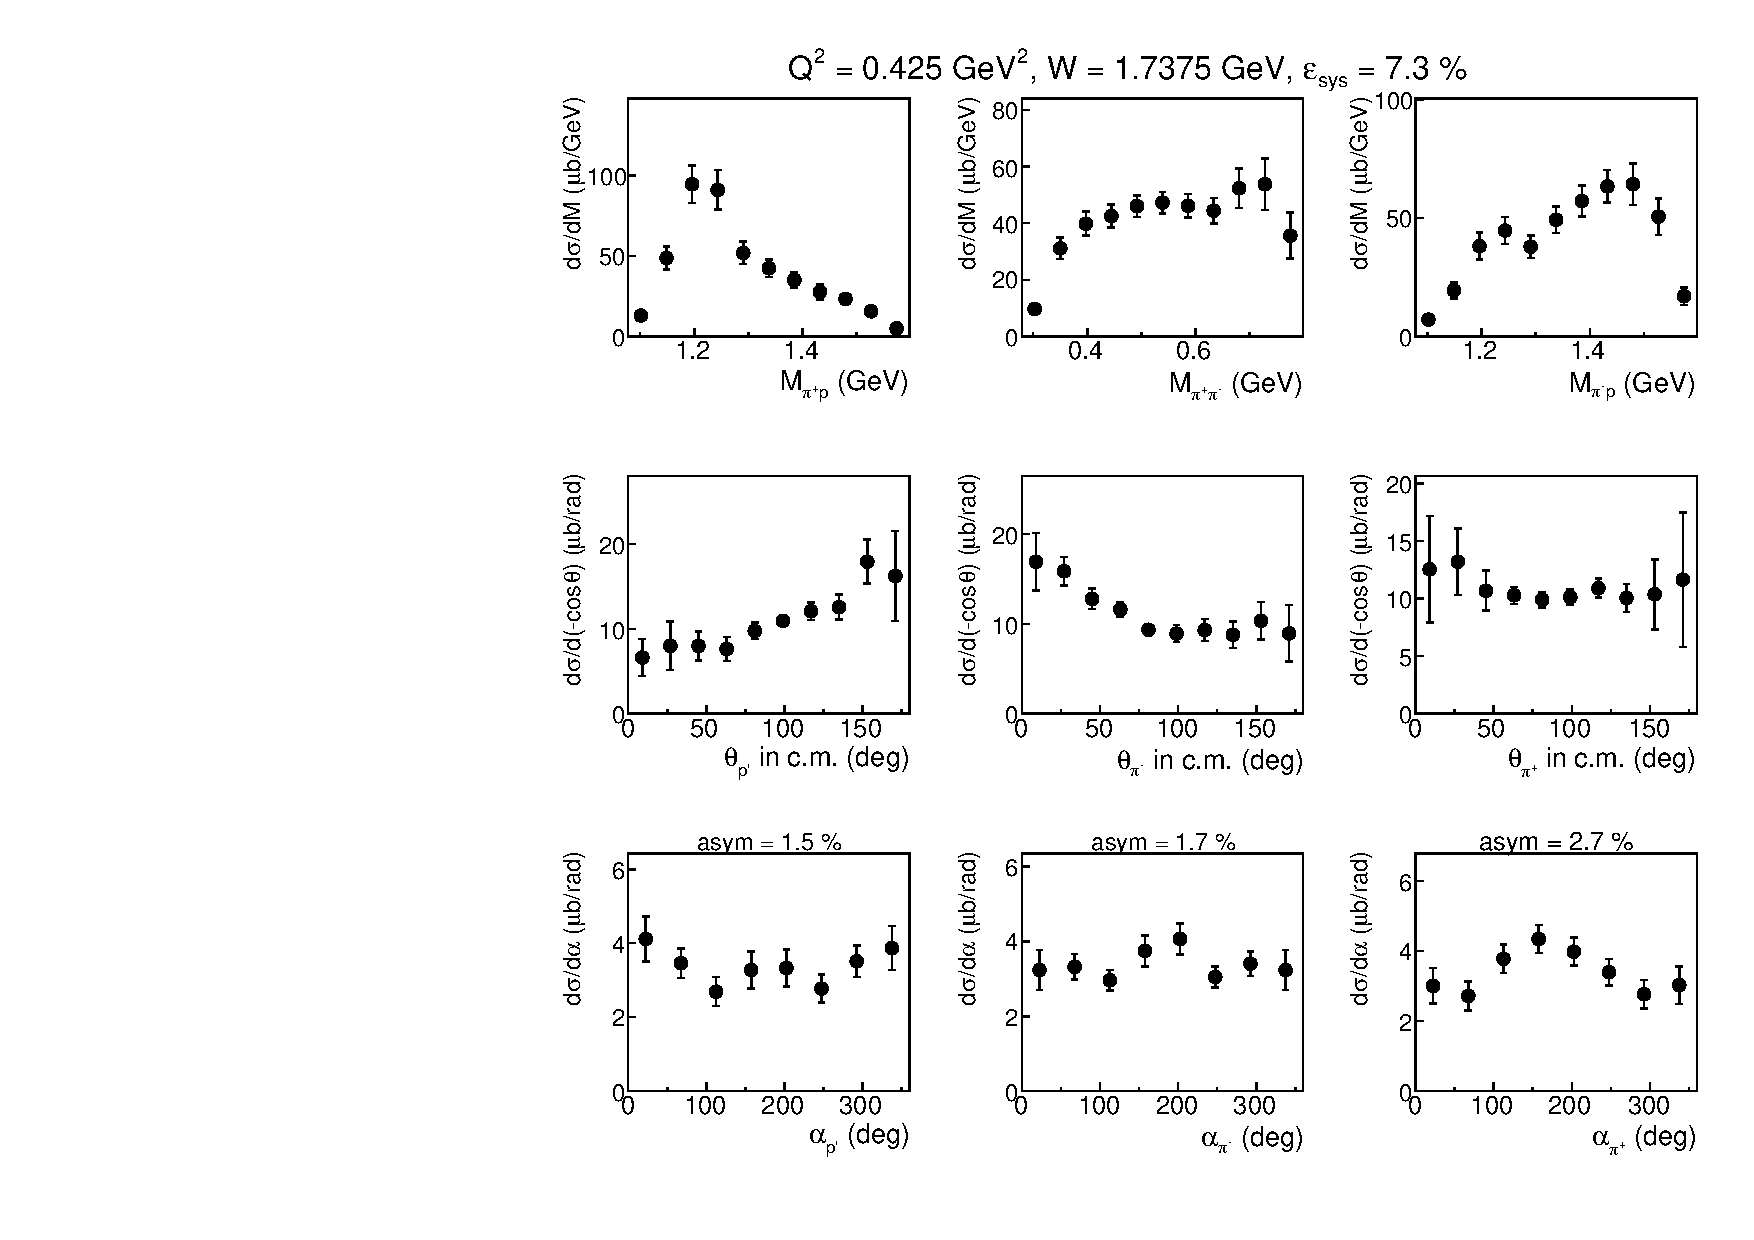
\includegraphics[width=0.495\textwidth]{pictures/appendix/1diff_distr/Q2_425/w_17375.pdf}}
\frame{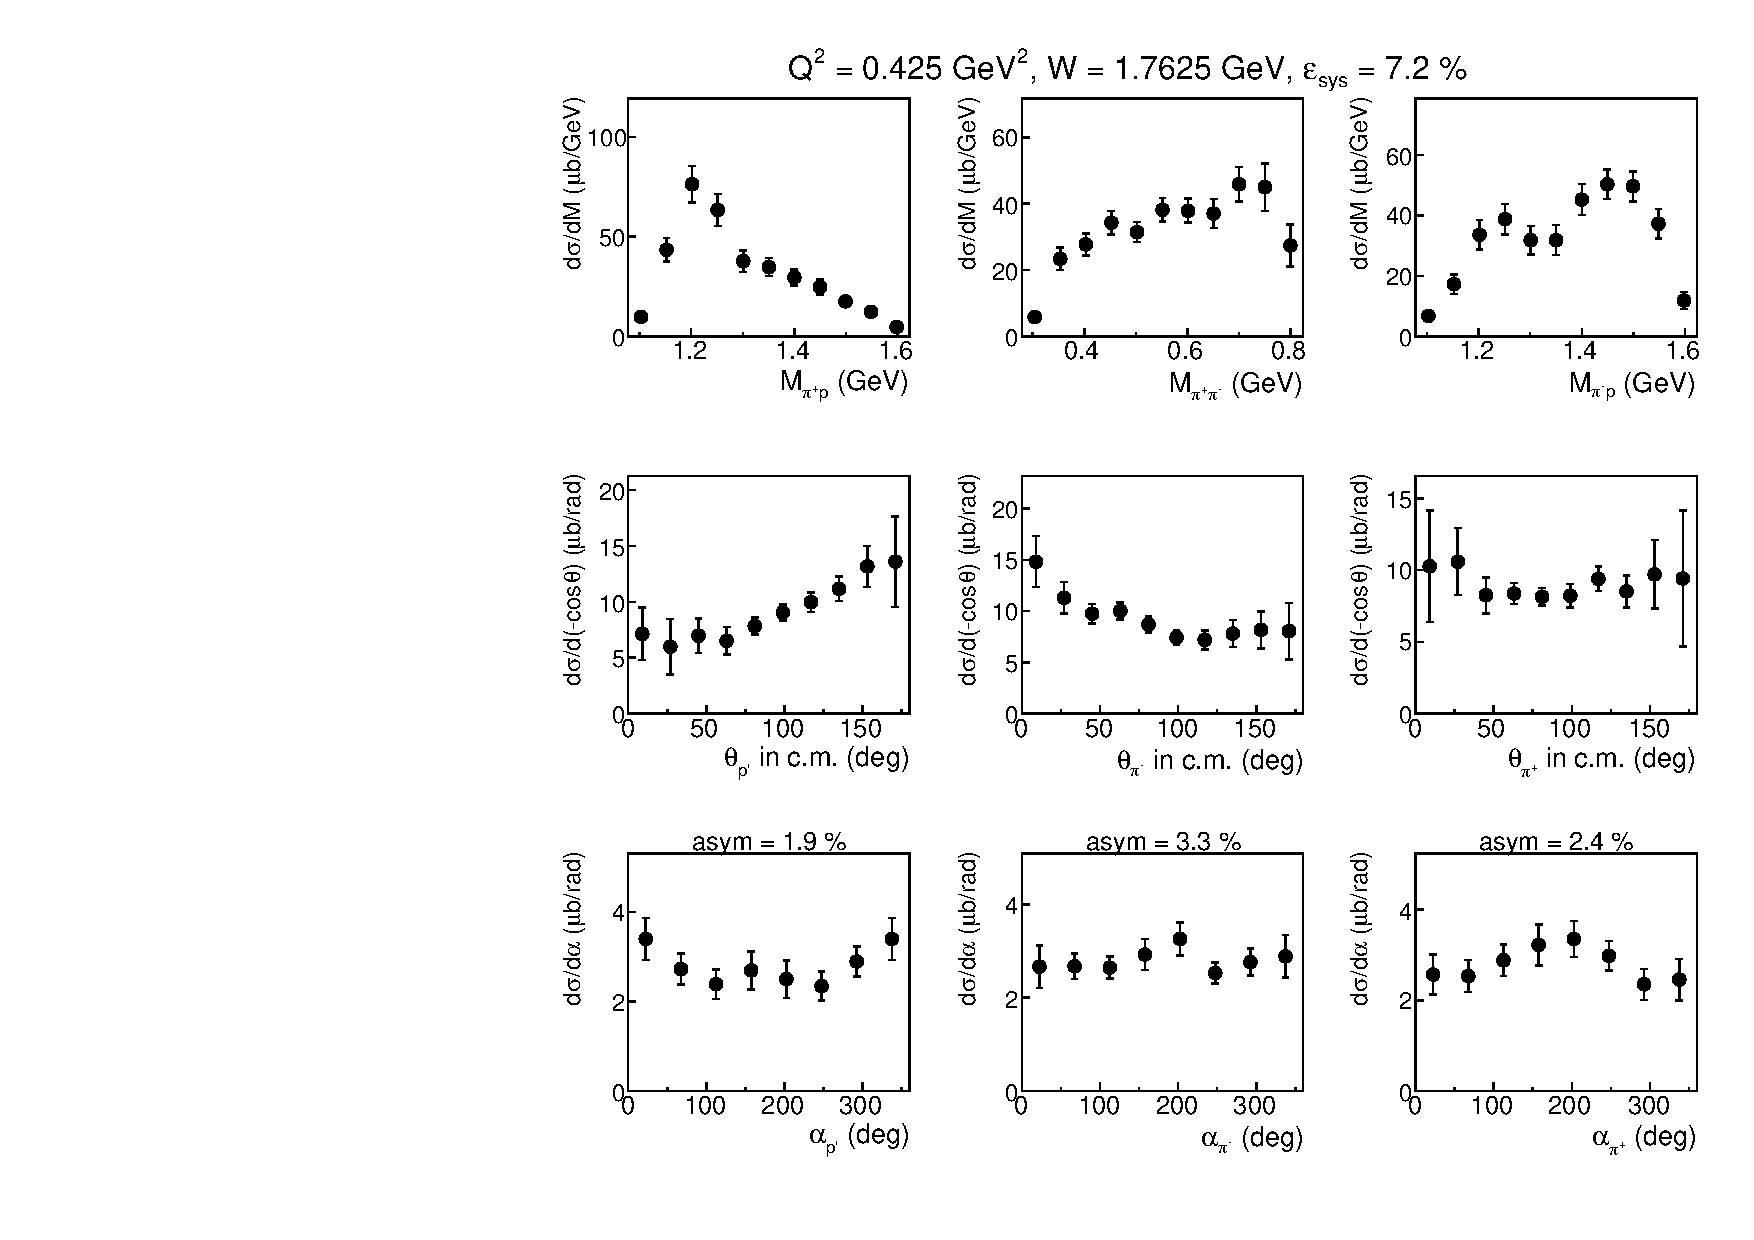
\includegraphics[width=0.495\textwidth]{pictures/appendix/1diff_distr/Q2_425/w_17625.pdf}}
\frame{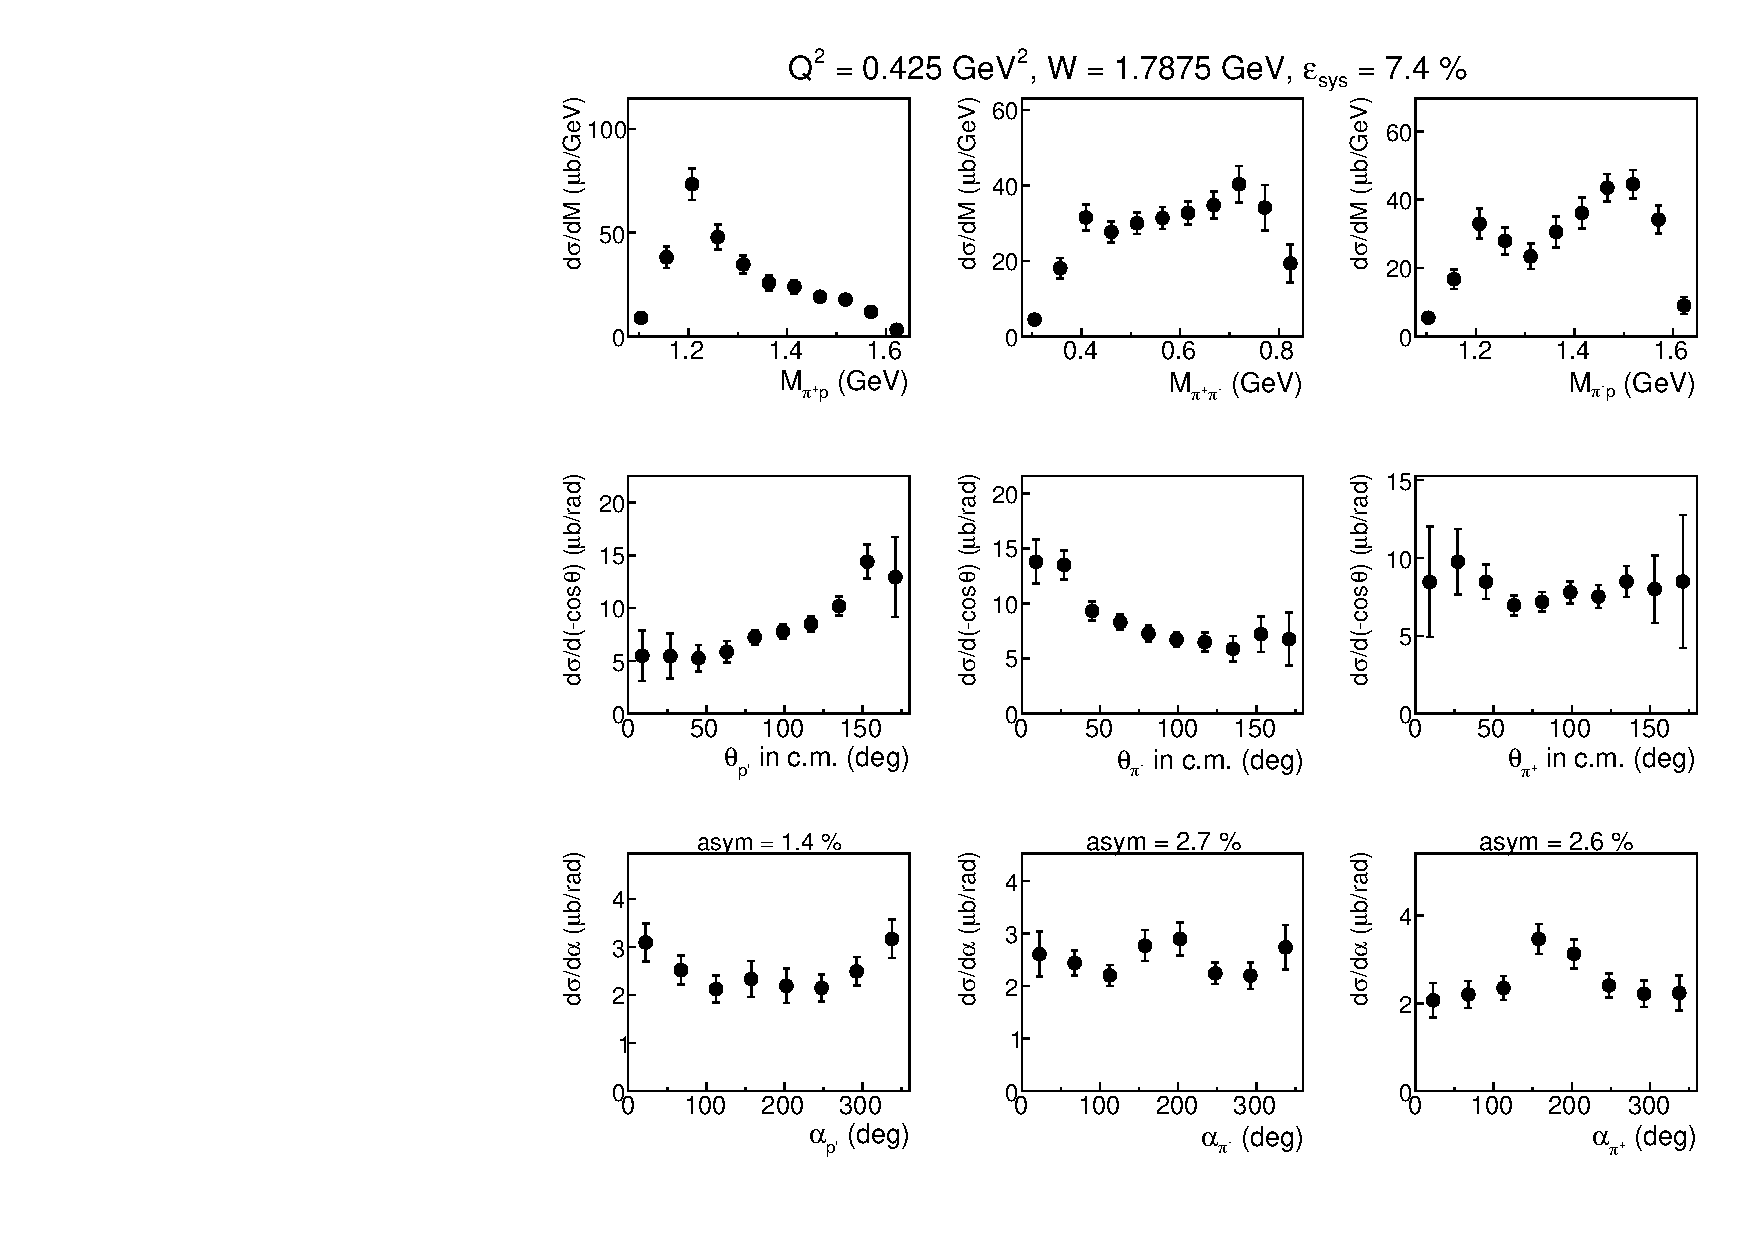
\includegraphics[width=0.495\textwidth]{pictures/appendix/1diff_distr/Q2_425/w_17875.pdf}}
\frame{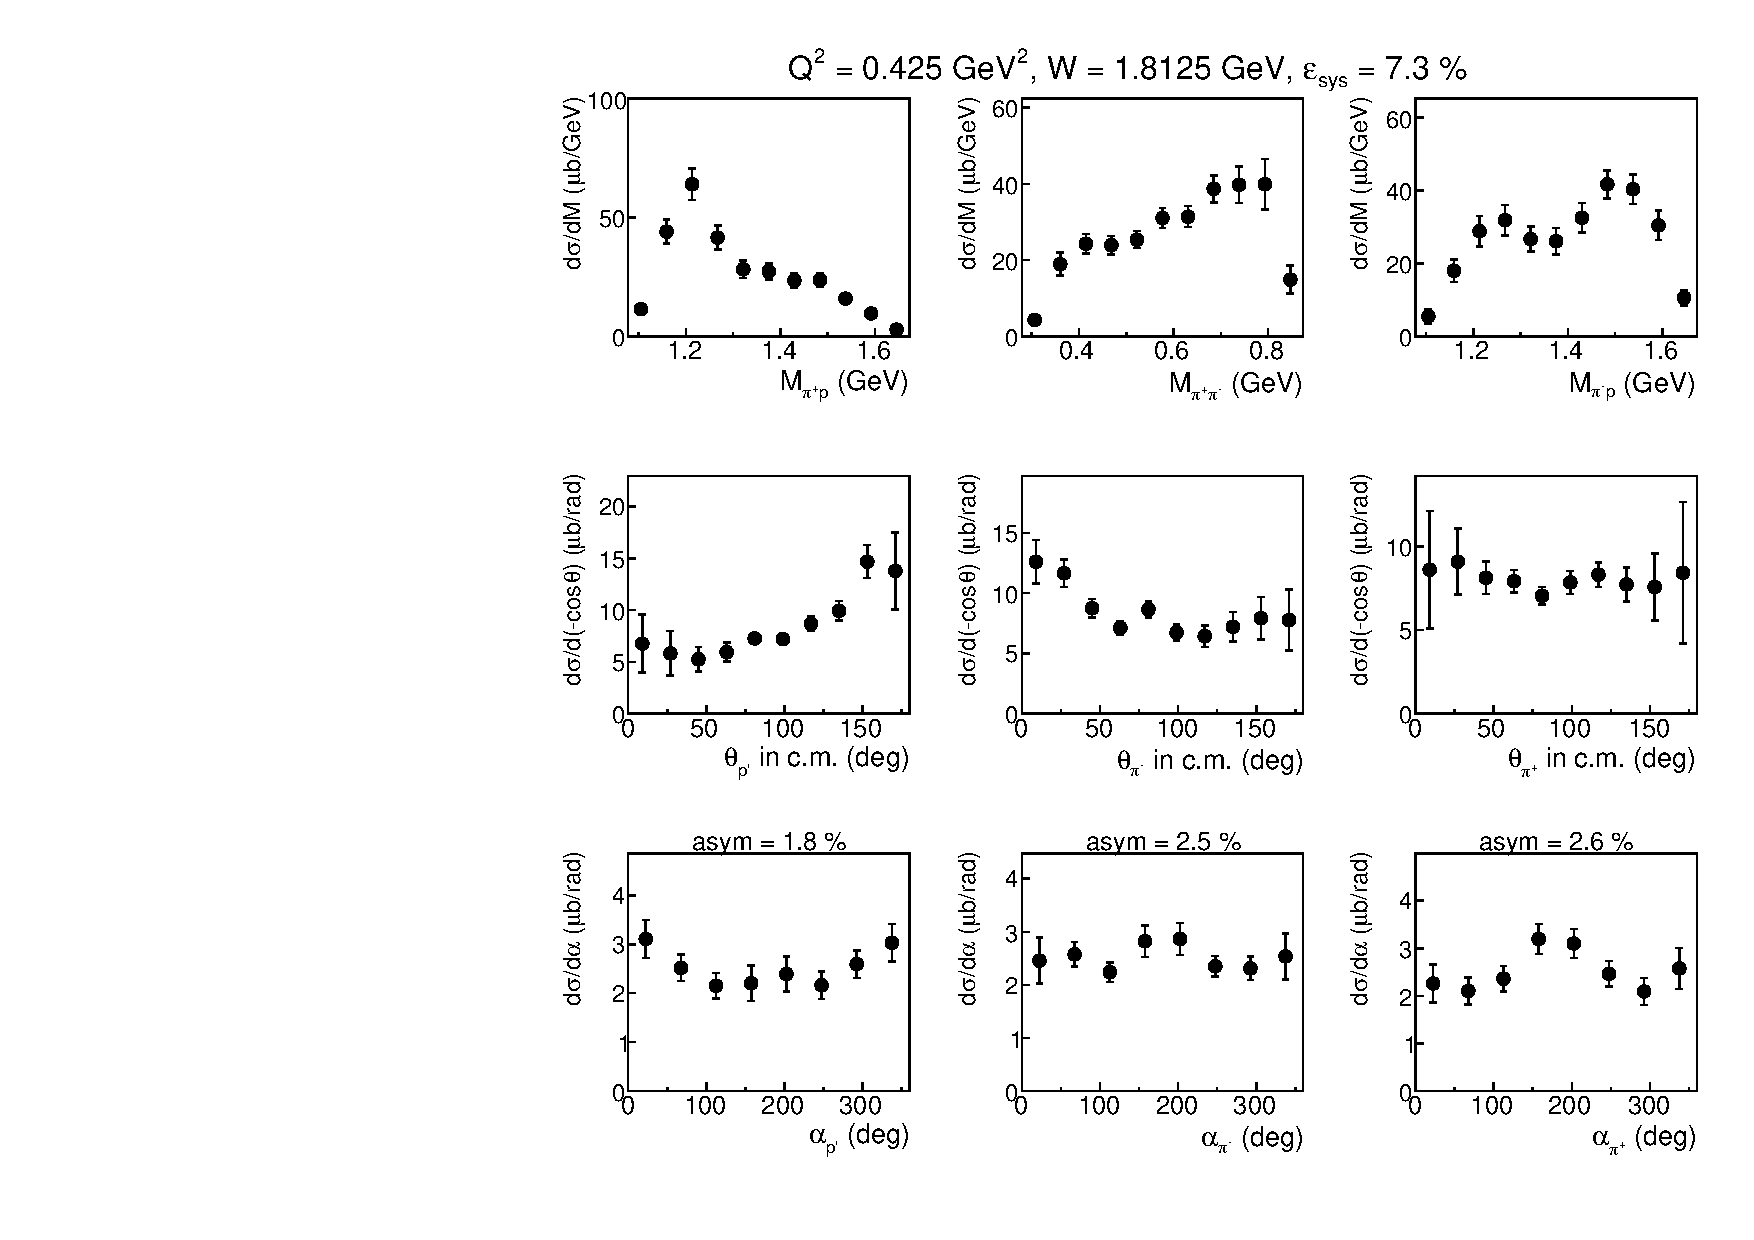
\includegraphics[width=0.495\textwidth]{pictures/appendix/1diff_distr/Q2_425/w_18125.pdf}}
\frame{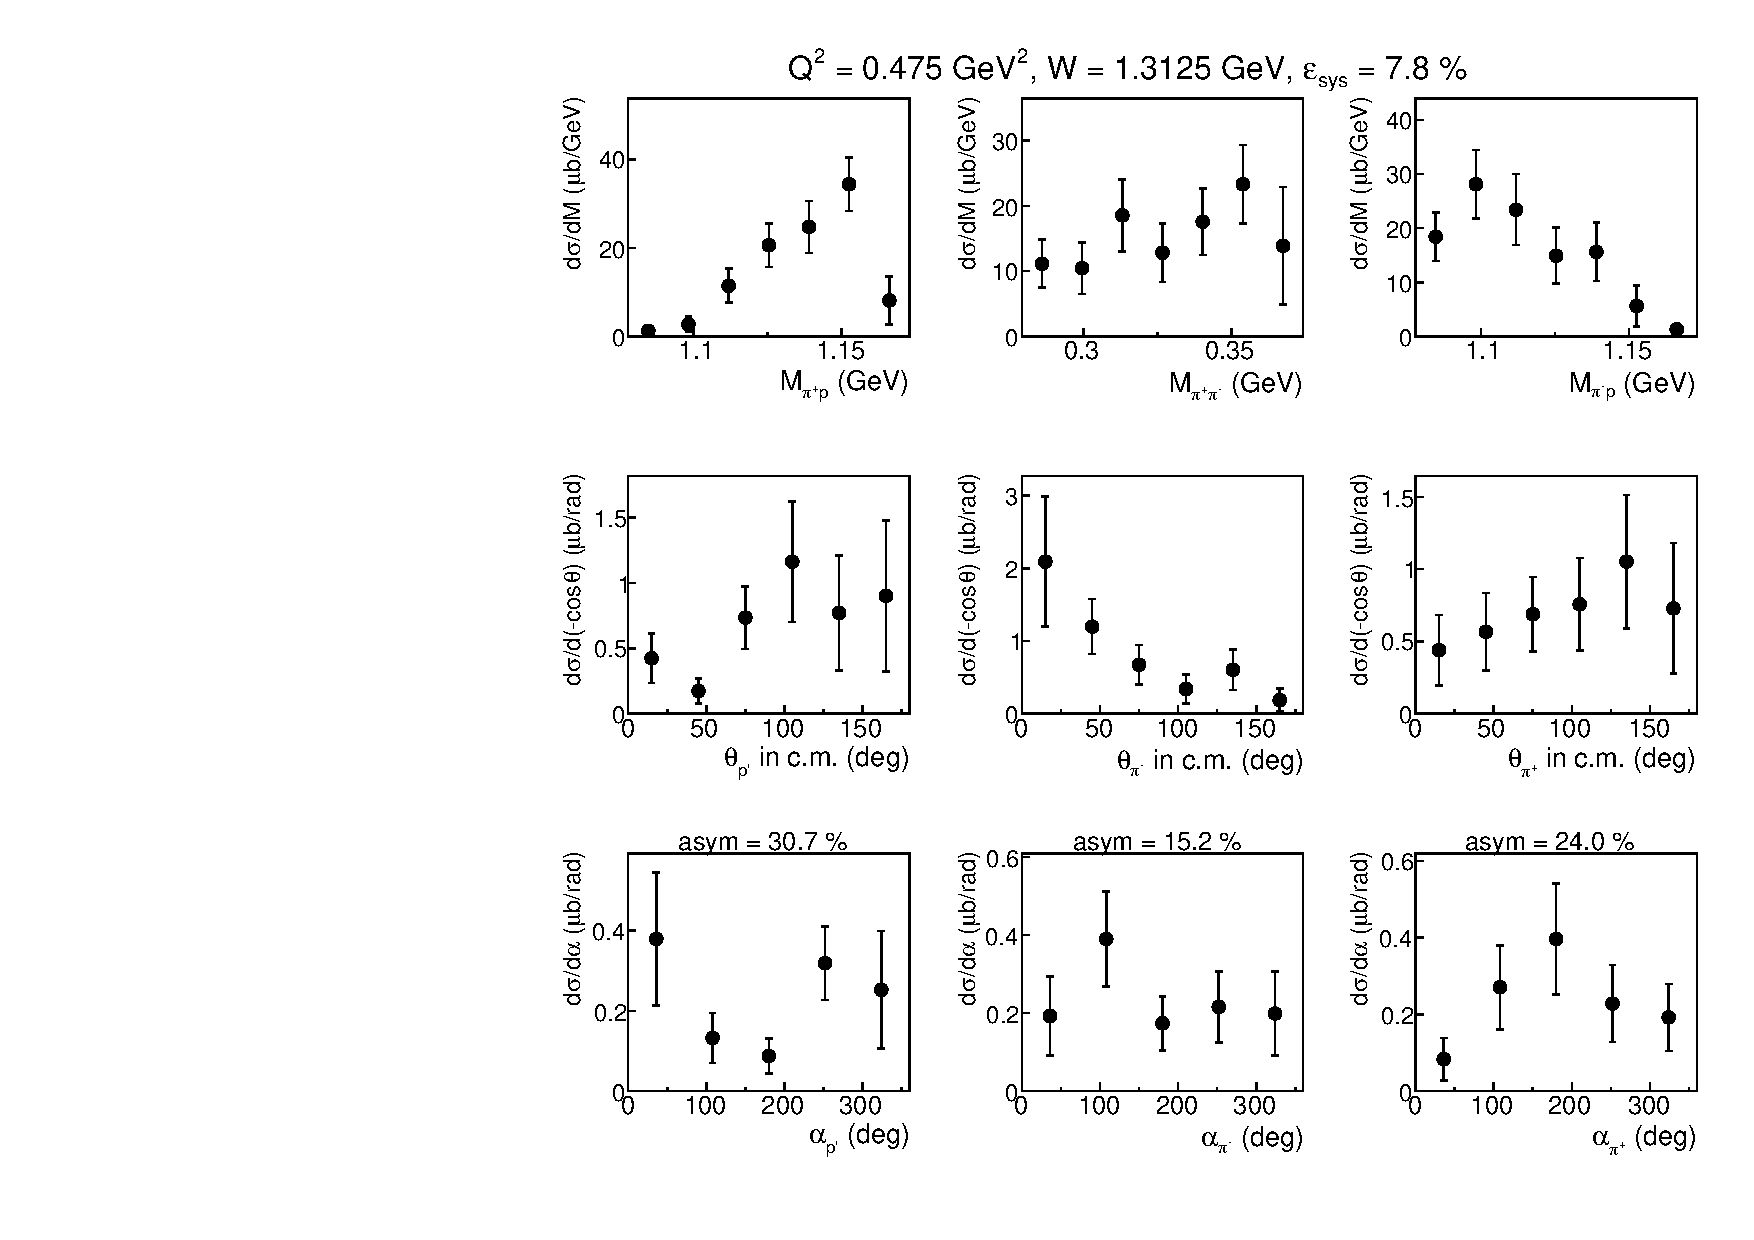
\includegraphics[width=0.495\textwidth]{pictures/appendix/1diff_distr/Q2_475/w_13125.pdf}}
\caption{\small Measured single-differential cross sections.} \label{fig:appx_2}
\end{center}
\end{figure}

\clearpage
\begin{figure}[htp]
\begin{center}
\frame{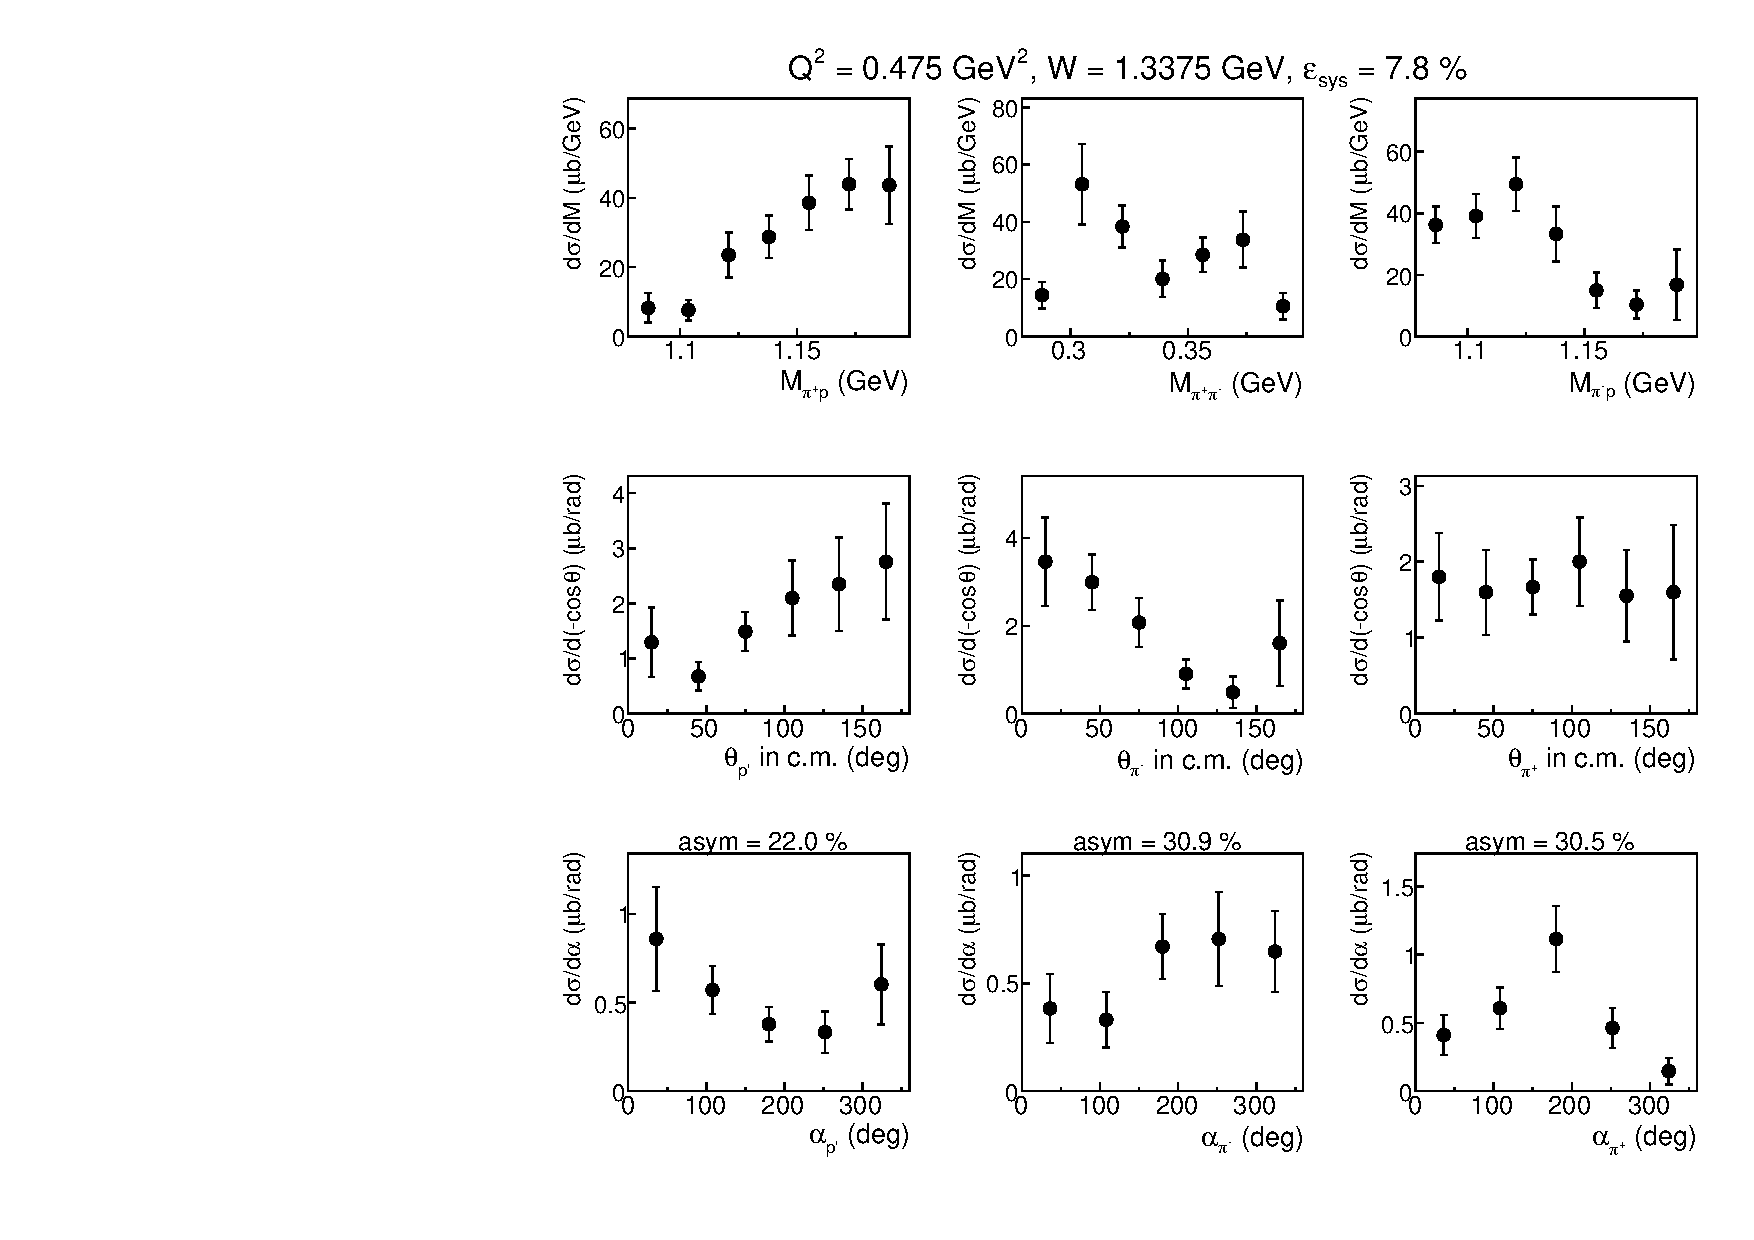
\includegraphics[width=0.495\textwidth]{pictures/appendix/1diff_distr/Q2_475/w_13375.pdf}}
\frame{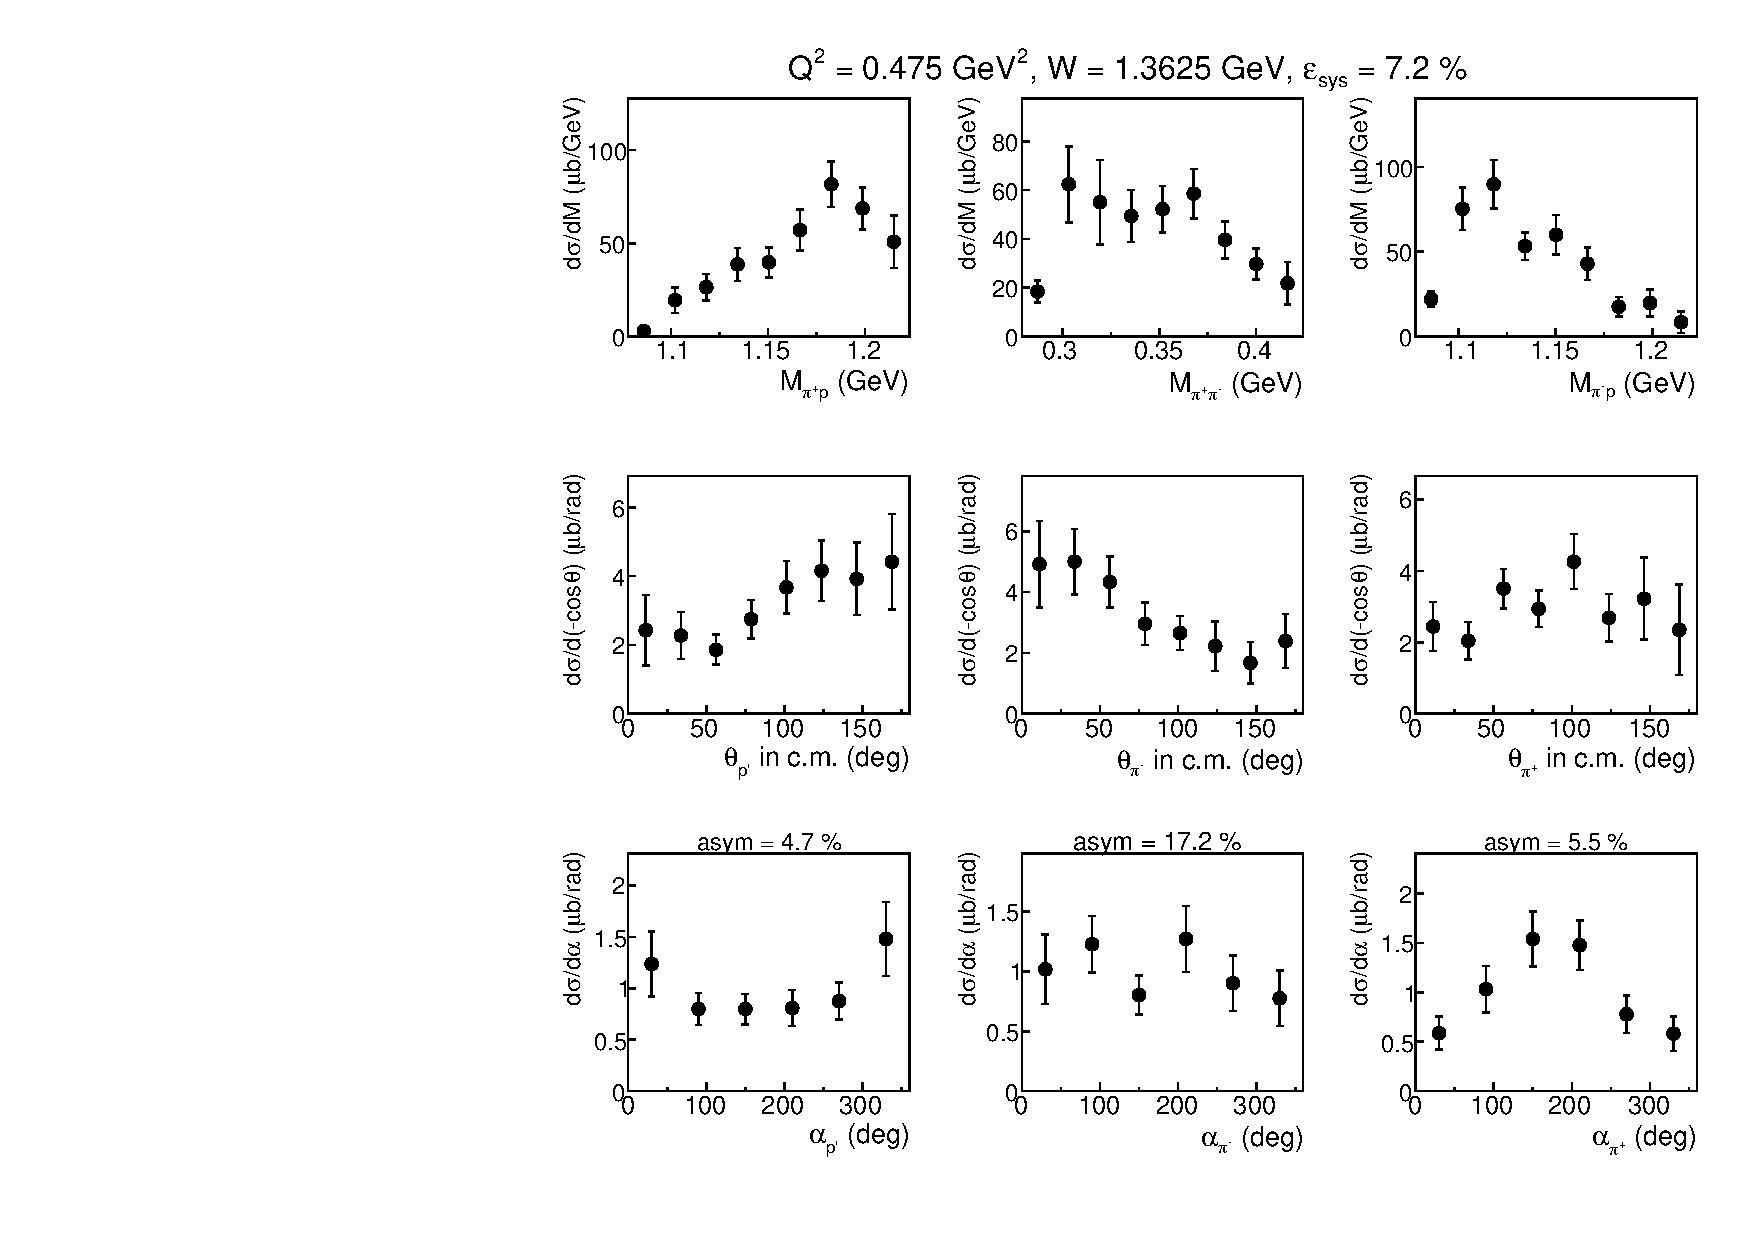
\includegraphics[width=0.495\textwidth]{pictures/appendix/1diff_distr/Q2_475/w_13625.pdf}}
\frame{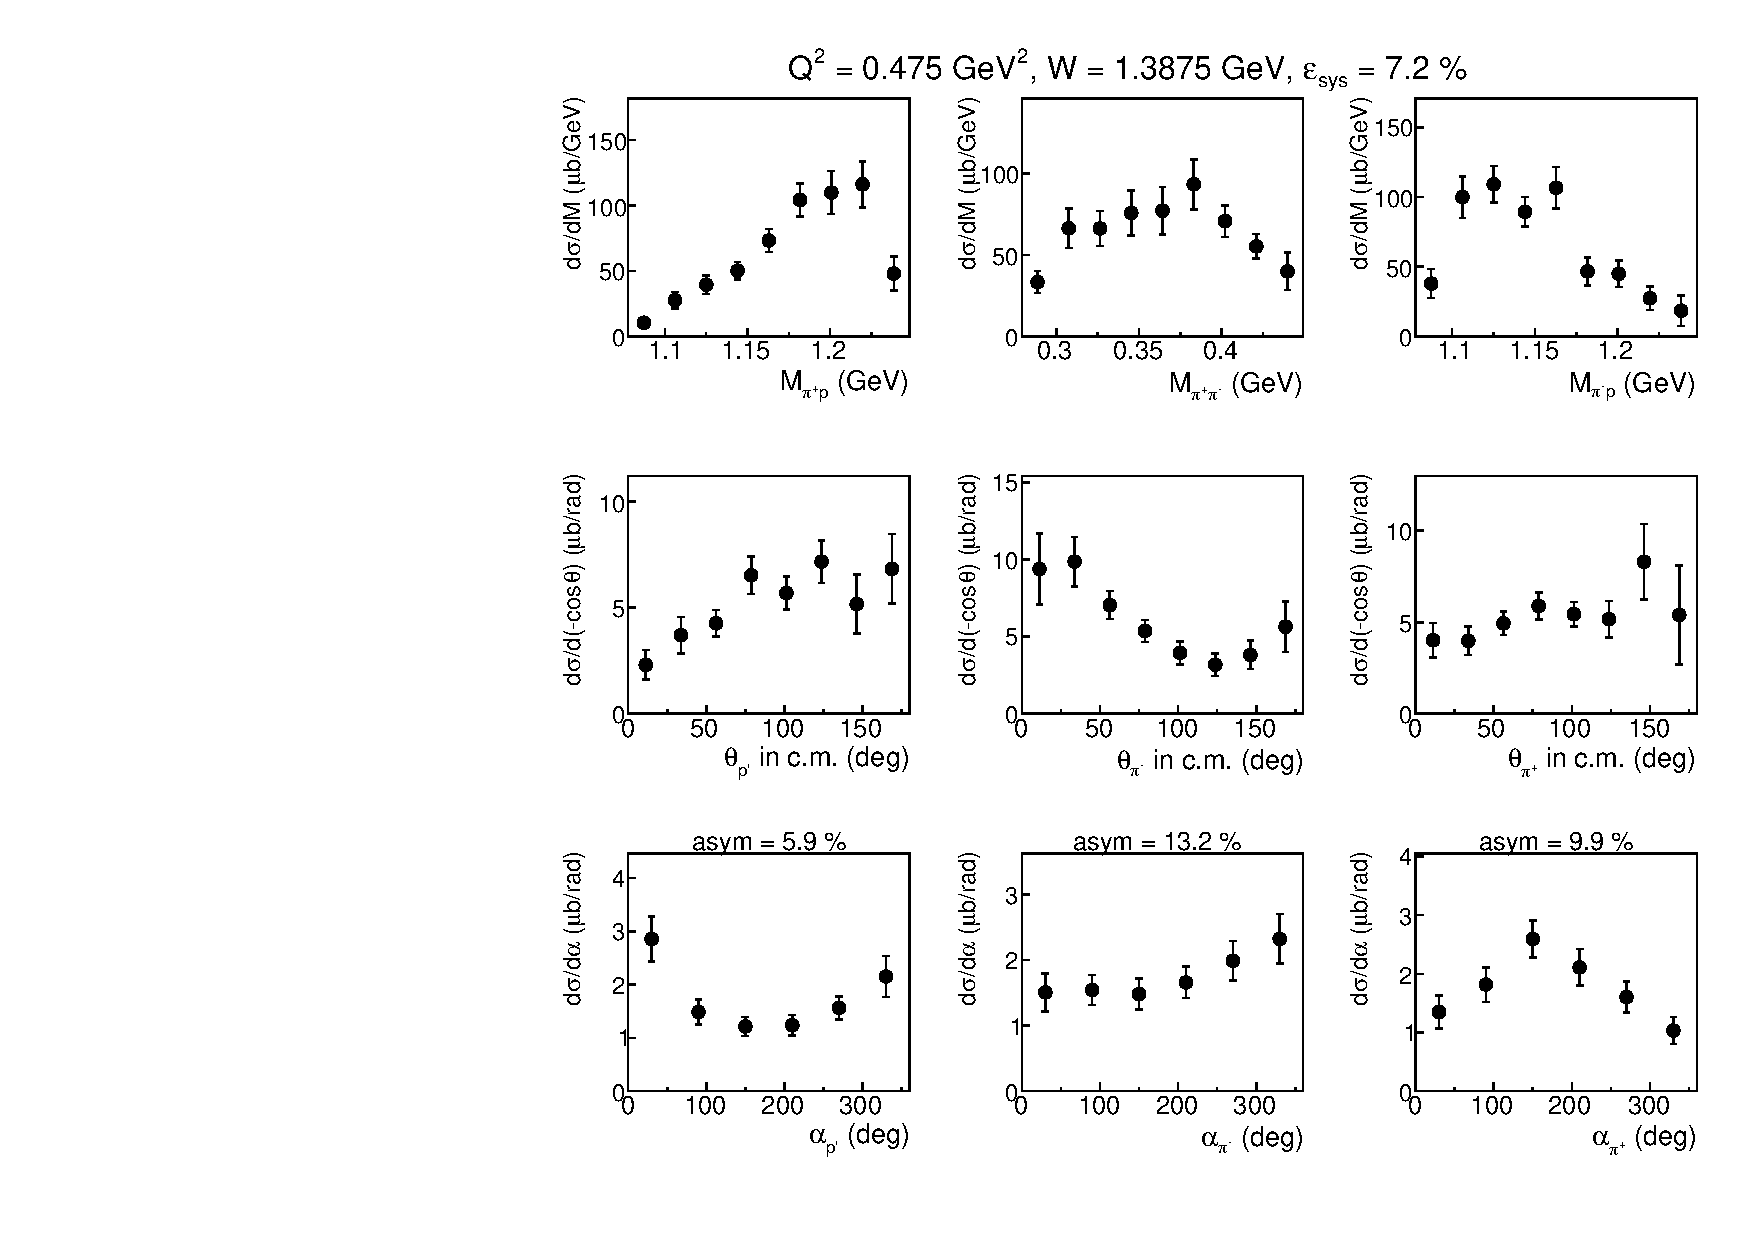
\includegraphics[width=0.495\textwidth]{pictures/appendix/1diff_distr/Q2_475/w_13875.pdf}}
\frame{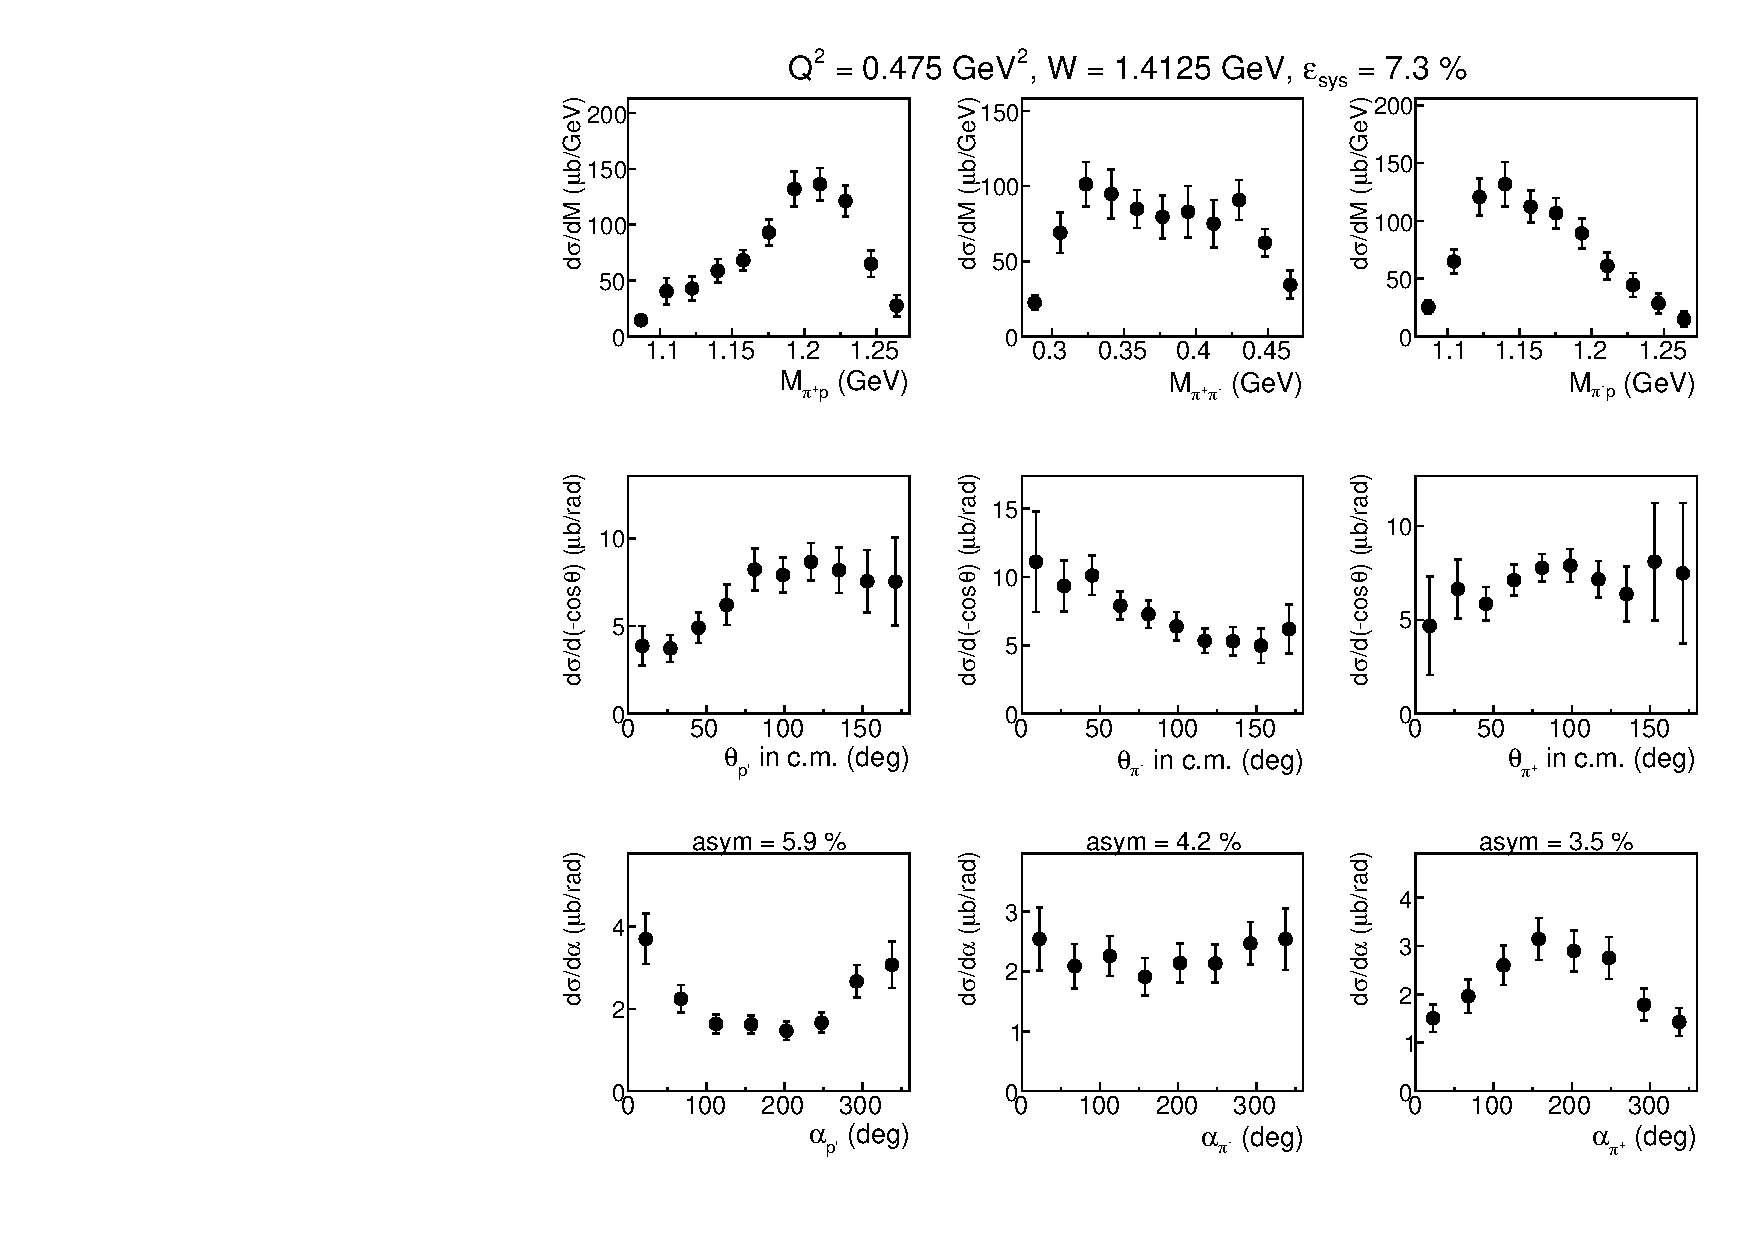
\includegraphics[width=0.495\textwidth]{pictures/appendix/1diff_distr/Q2_475/w_14125.pdf}}
\frame{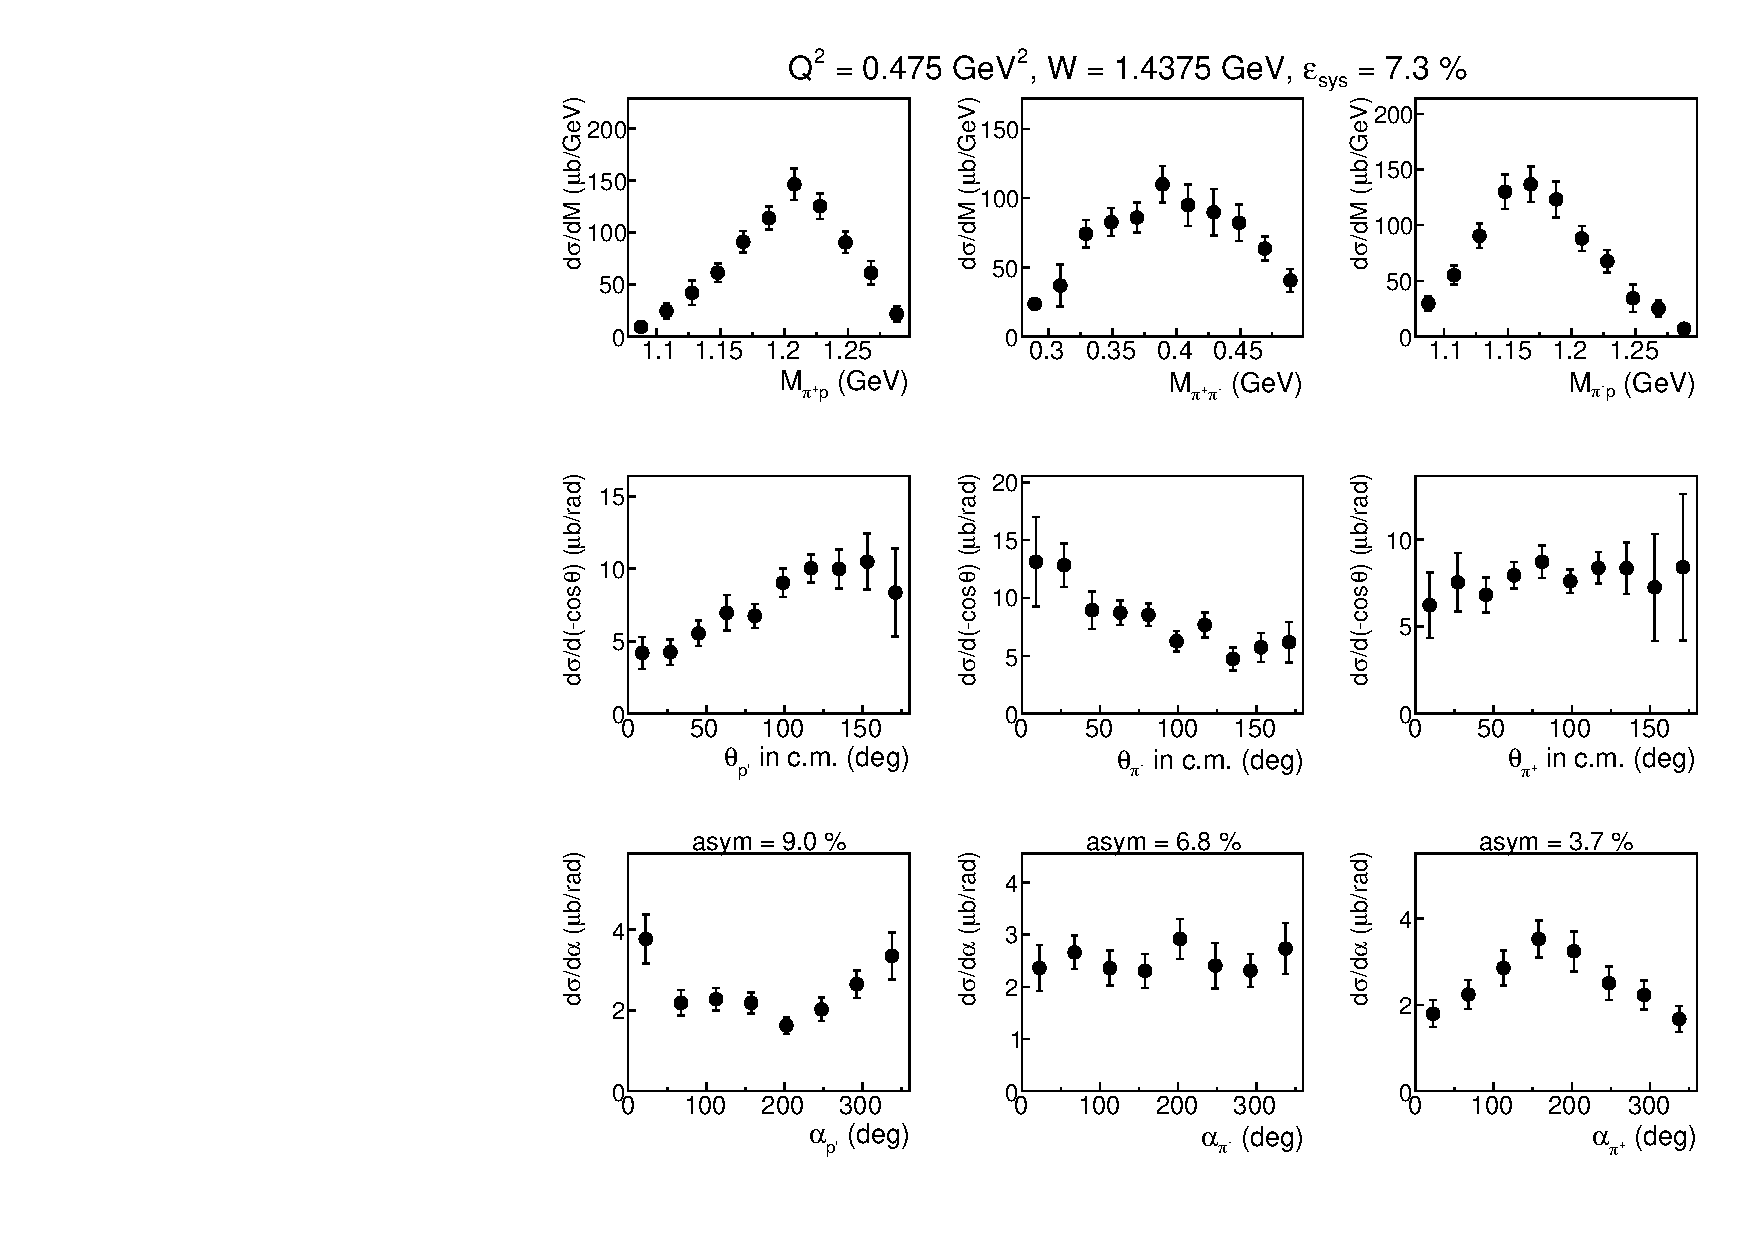
\includegraphics[width=0.495\textwidth]{pictures/appendix/1diff_distr/Q2_475/w_14375.pdf}}
\frame{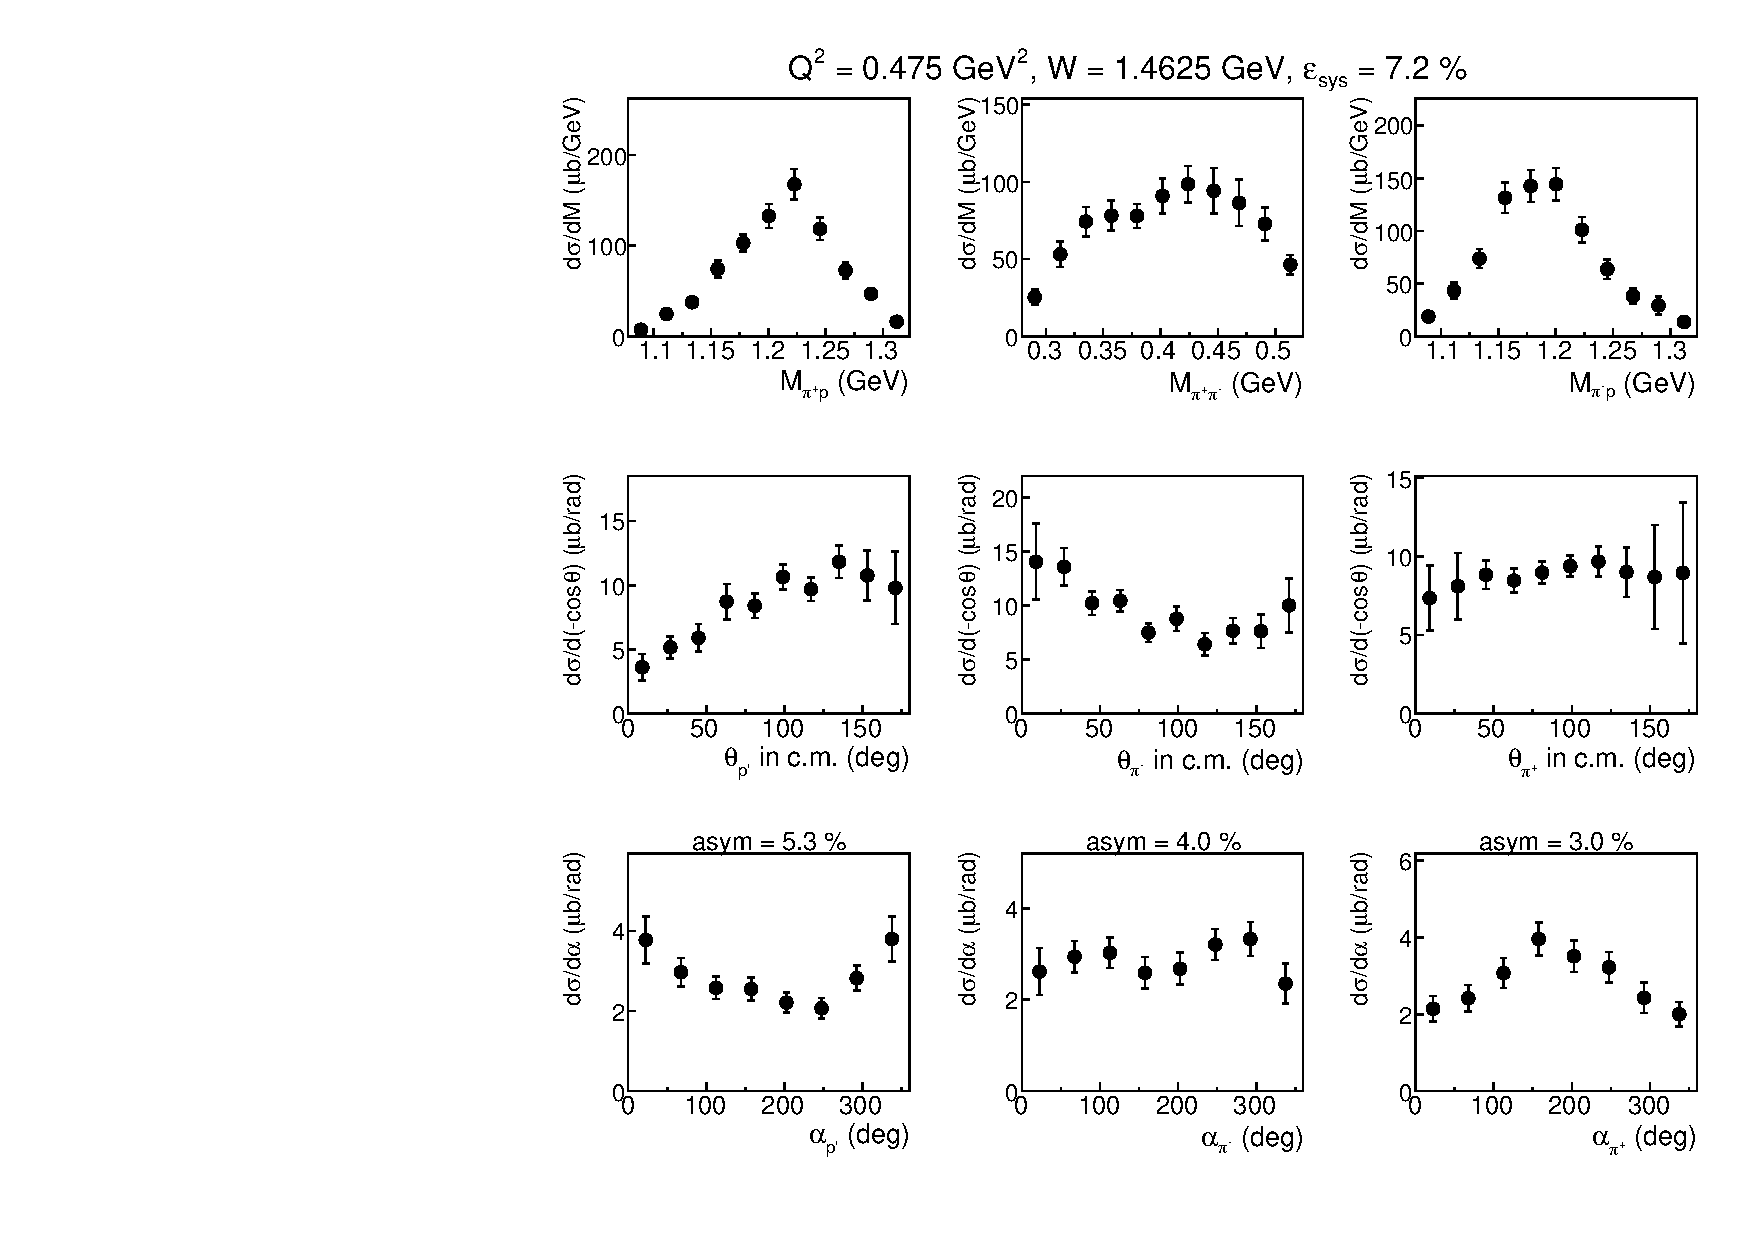
\includegraphics[width=0.495\textwidth]{pictures/appendix/1diff_distr/Q2_475/w_14625.pdf}}
\caption{\small Measured single-differential cross sections.} \label{fig:appx_3}
\end{center}
\end{figure}

\clearpage
\begin{figure}[htp]
\begin{center}
\frame{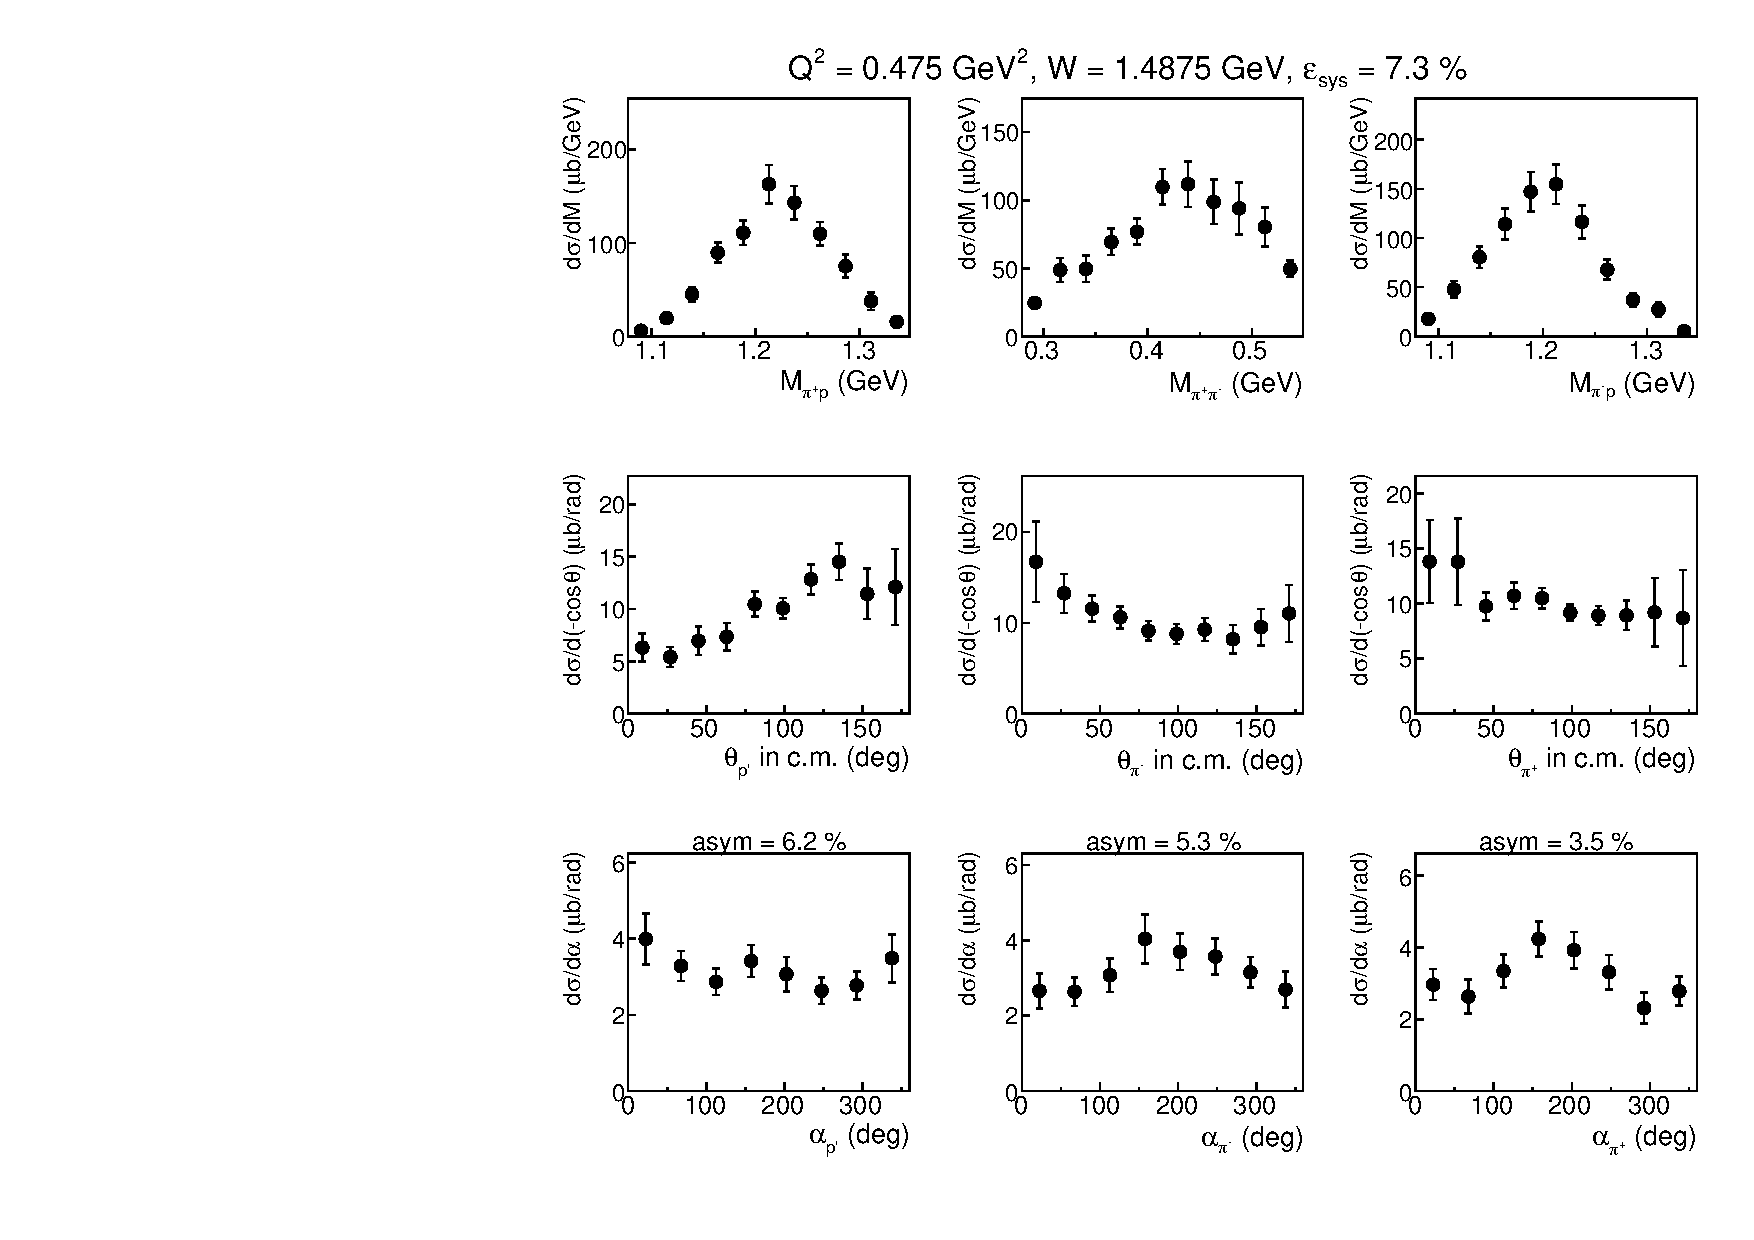
\includegraphics[width=0.495\textwidth]{pictures/appendix/1diff_distr/Q2_475/w_14875.pdf}}
\frame{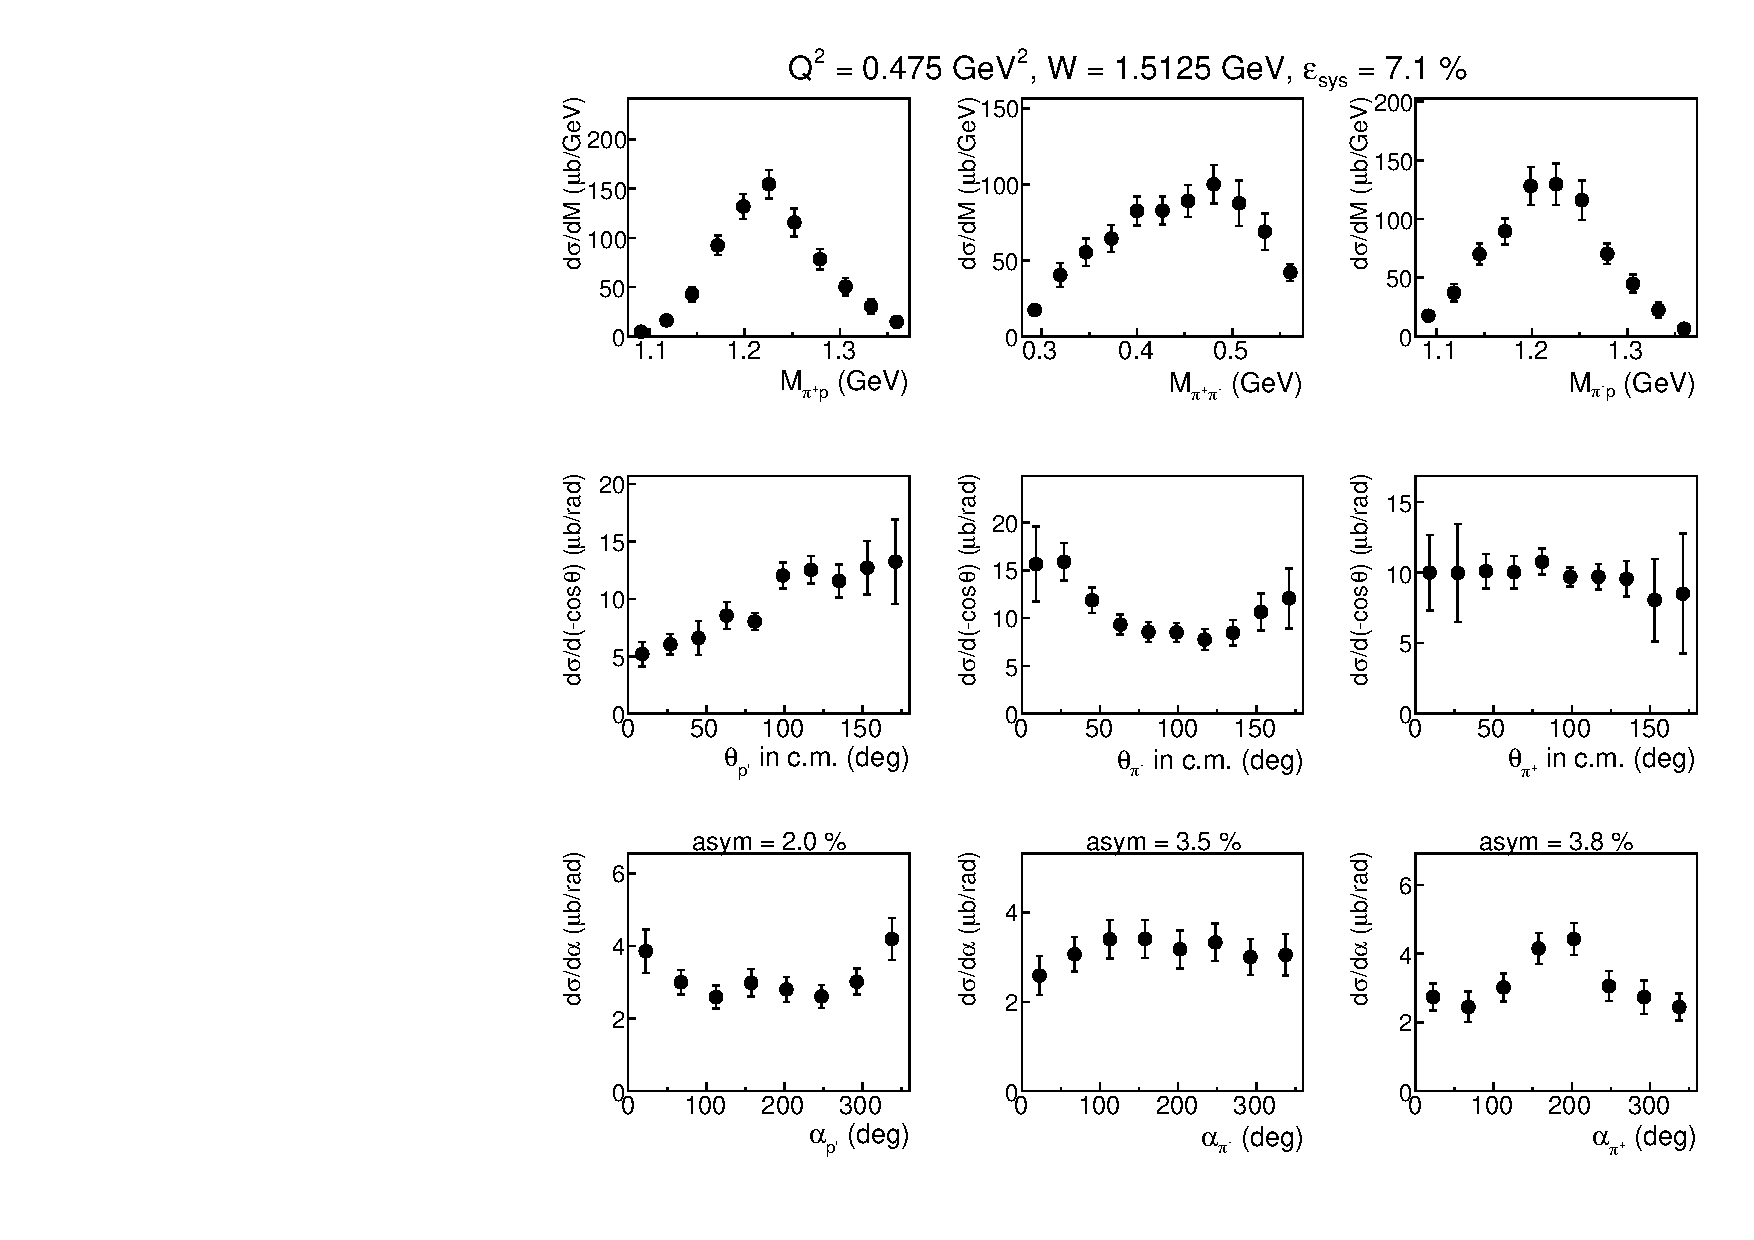
\includegraphics[width=0.495\textwidth]{pictures/appendix/1diff_distr/Q2_475/w_15125.pdf}}
\frame{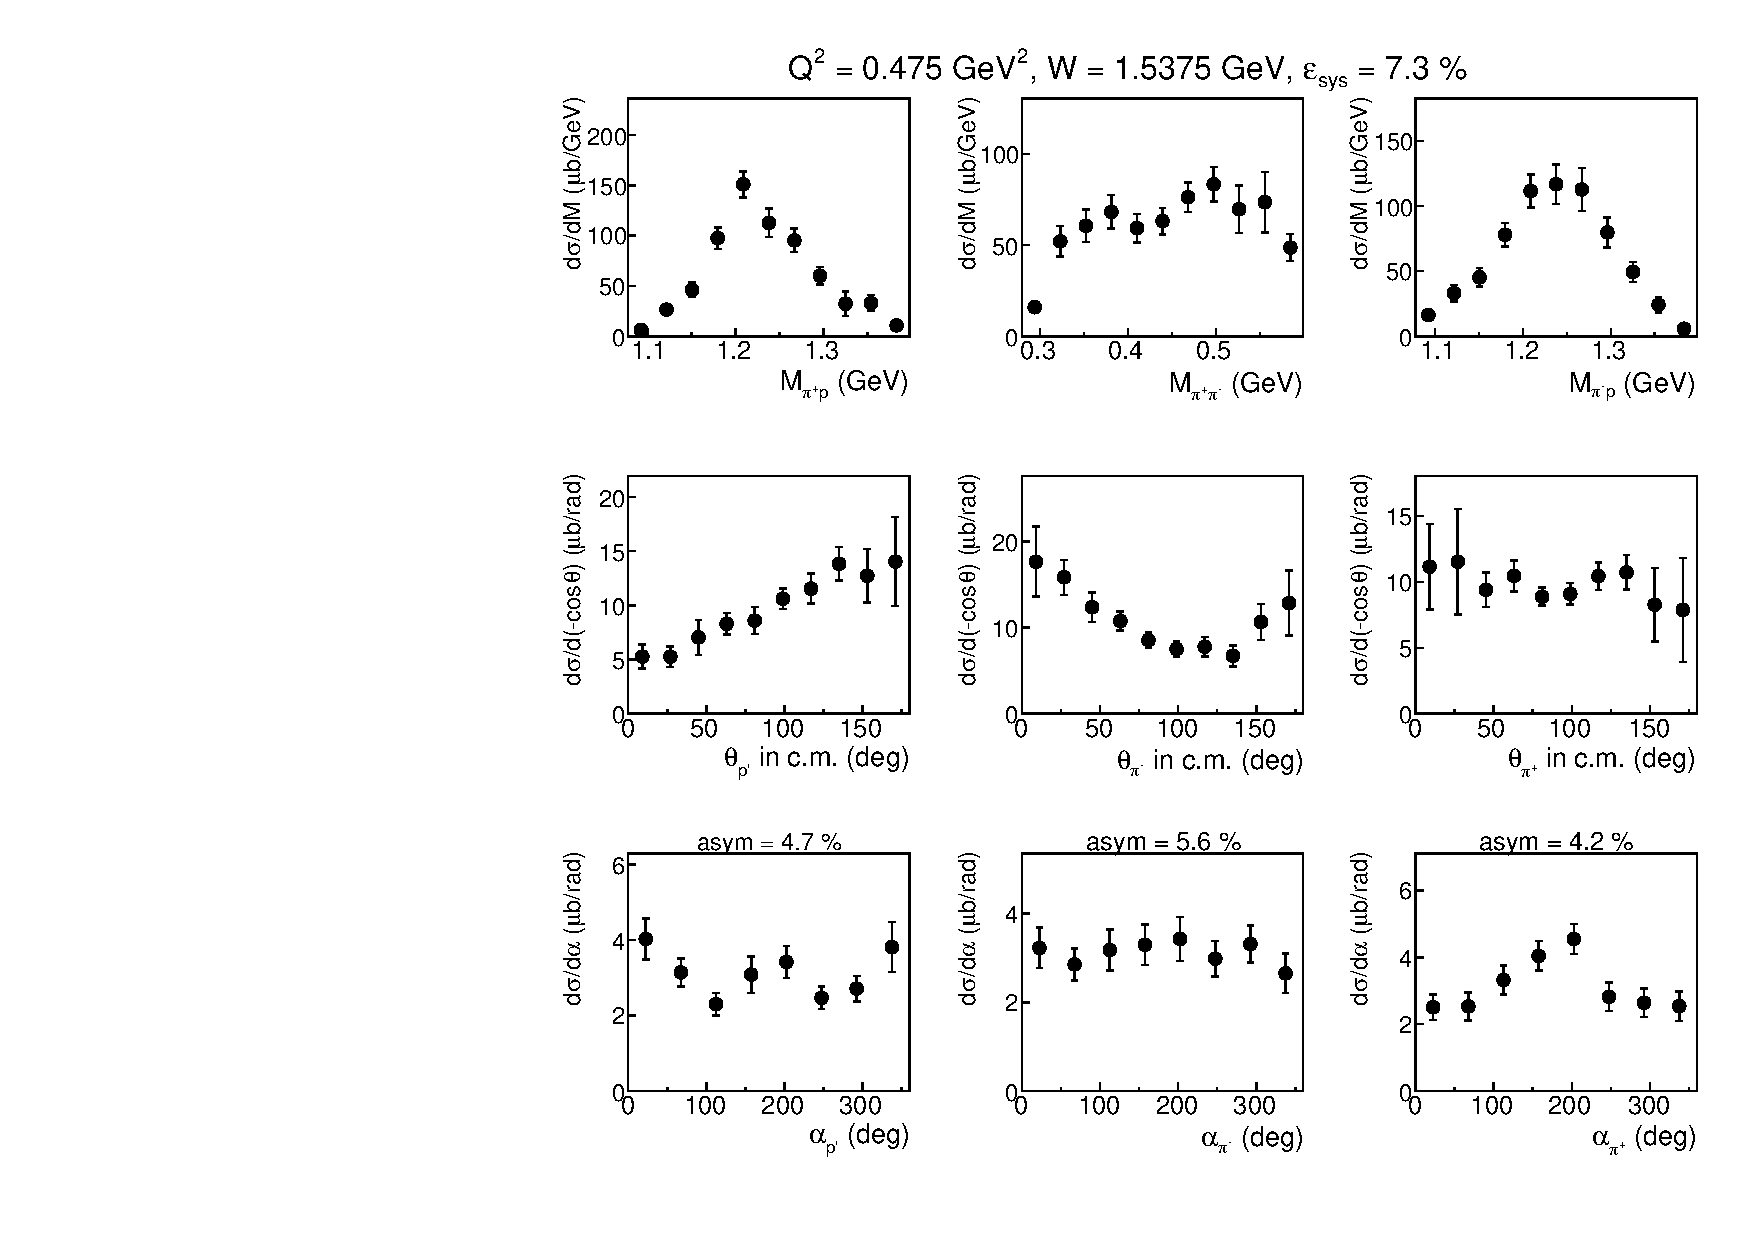
\includegraphics[width=0.495\textwidth]{pictures/appendix/1diff_distr/Q2_475/w_15375.pdf}}
\frame{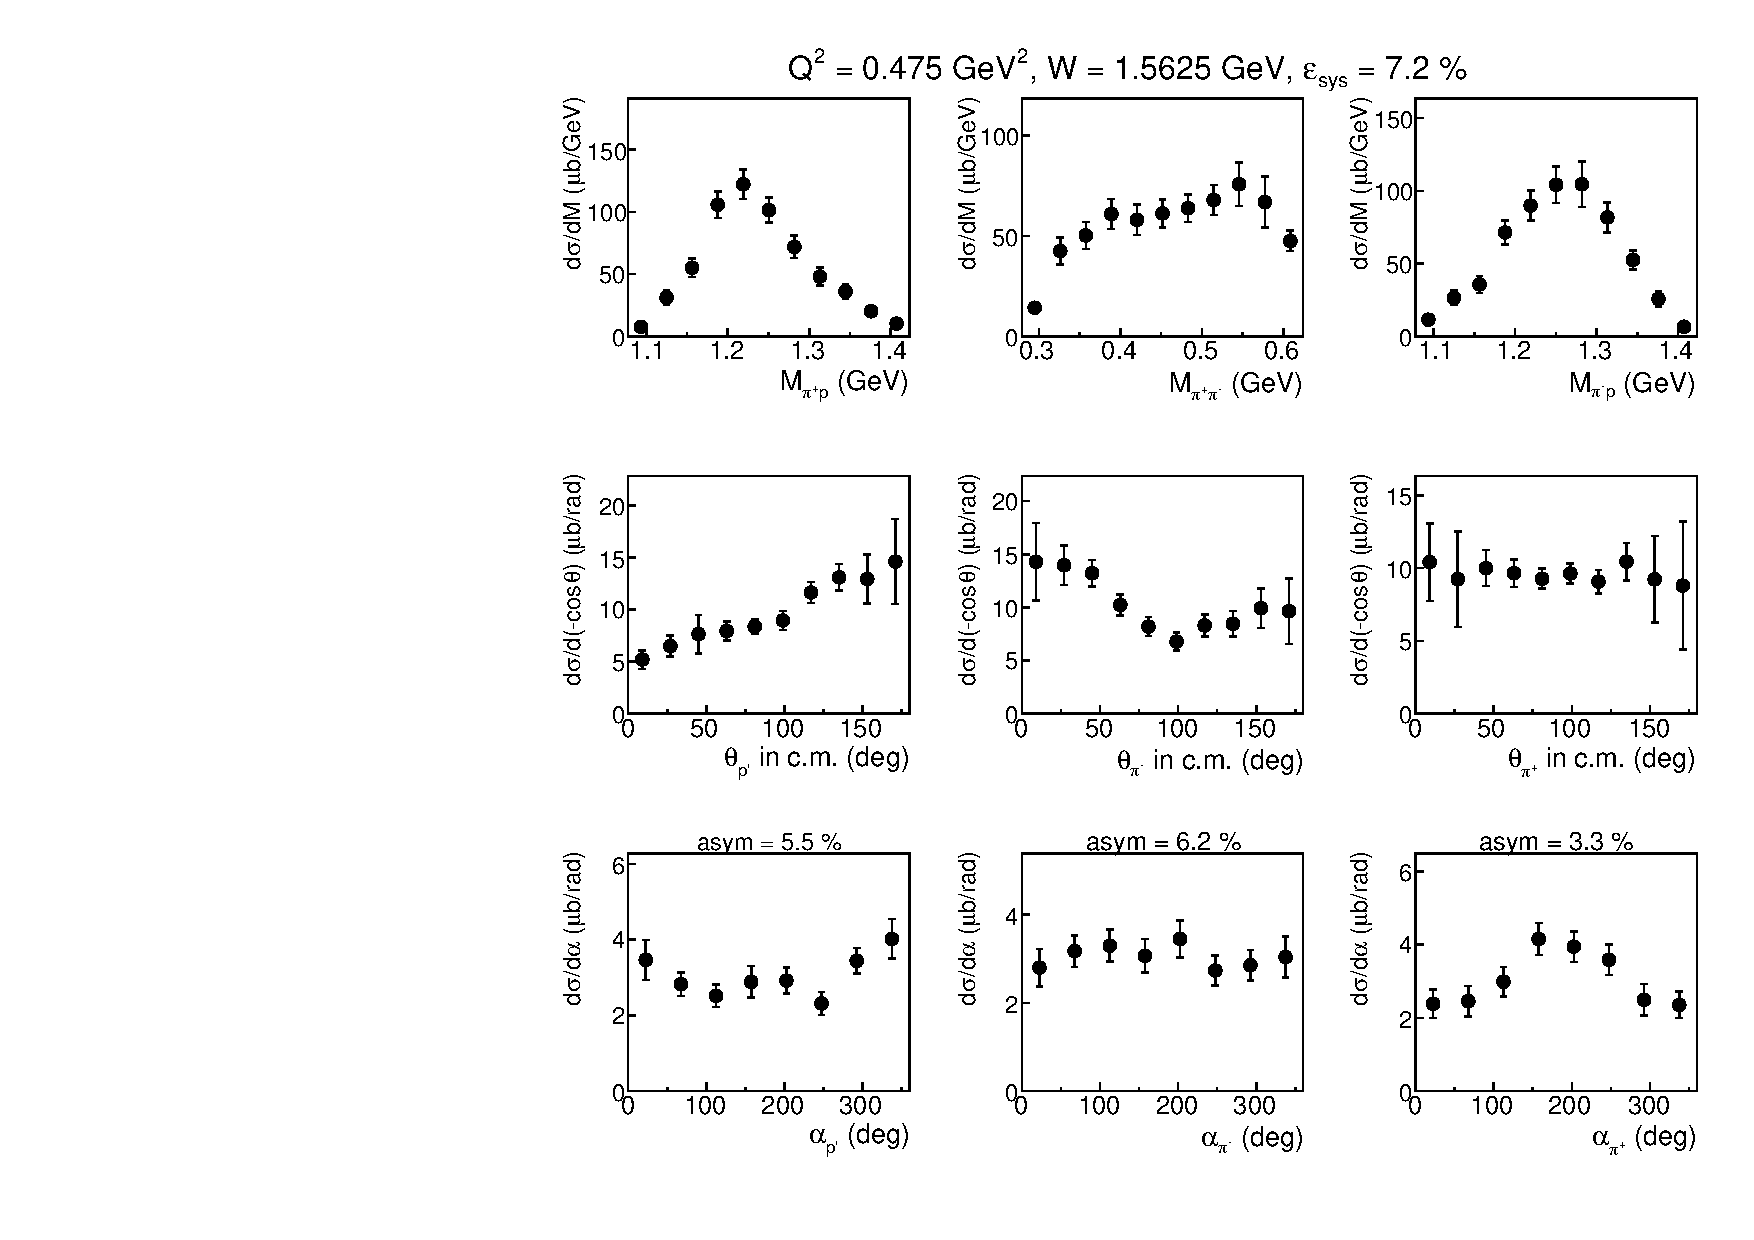
\includegraphics[width=0.495\textwidth]{pictures/appendix/1diff_distr/Q2_475/w_15625.pdf}}
\frame{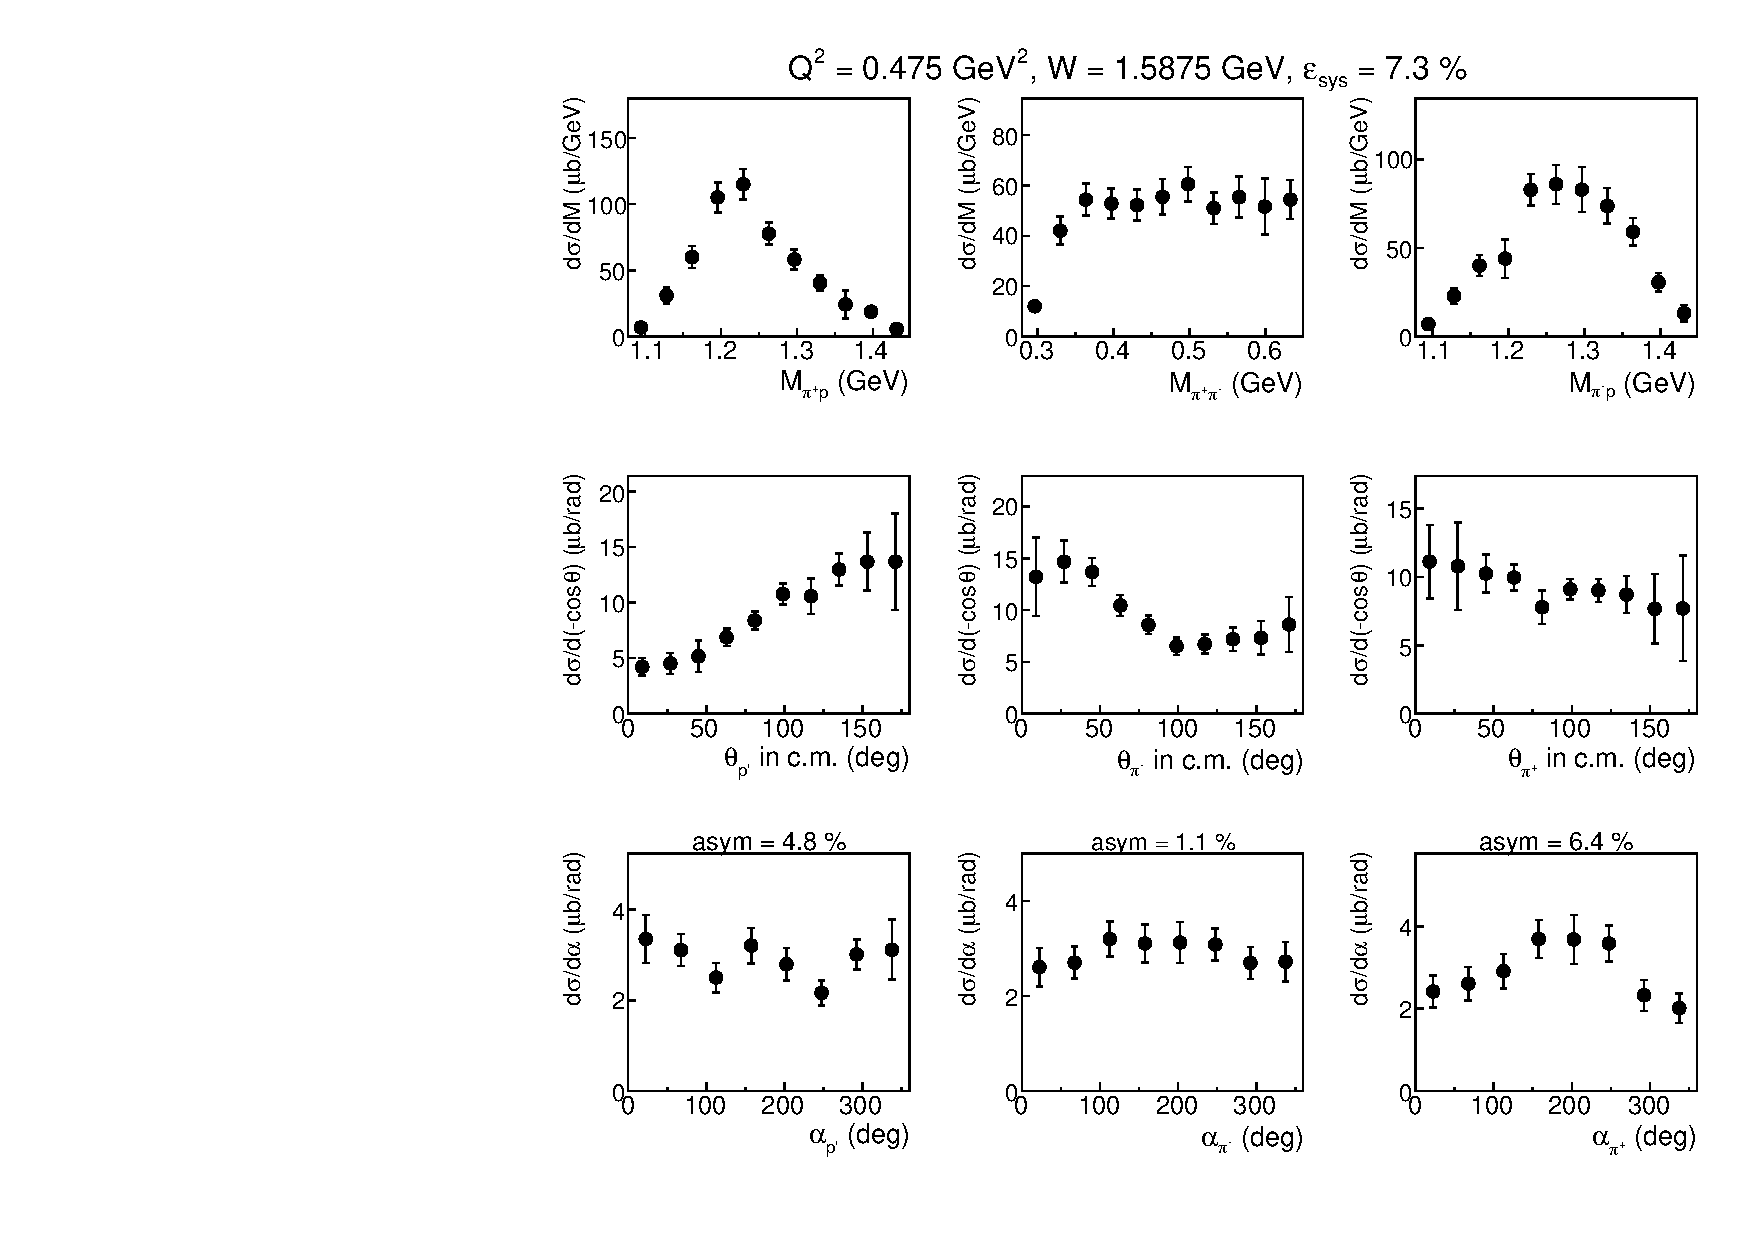
\includegraphics[width=0.495\textwidth]{pictures/appendix/1diff_distr/Q2_475/w_15875.pdf}}
\frame{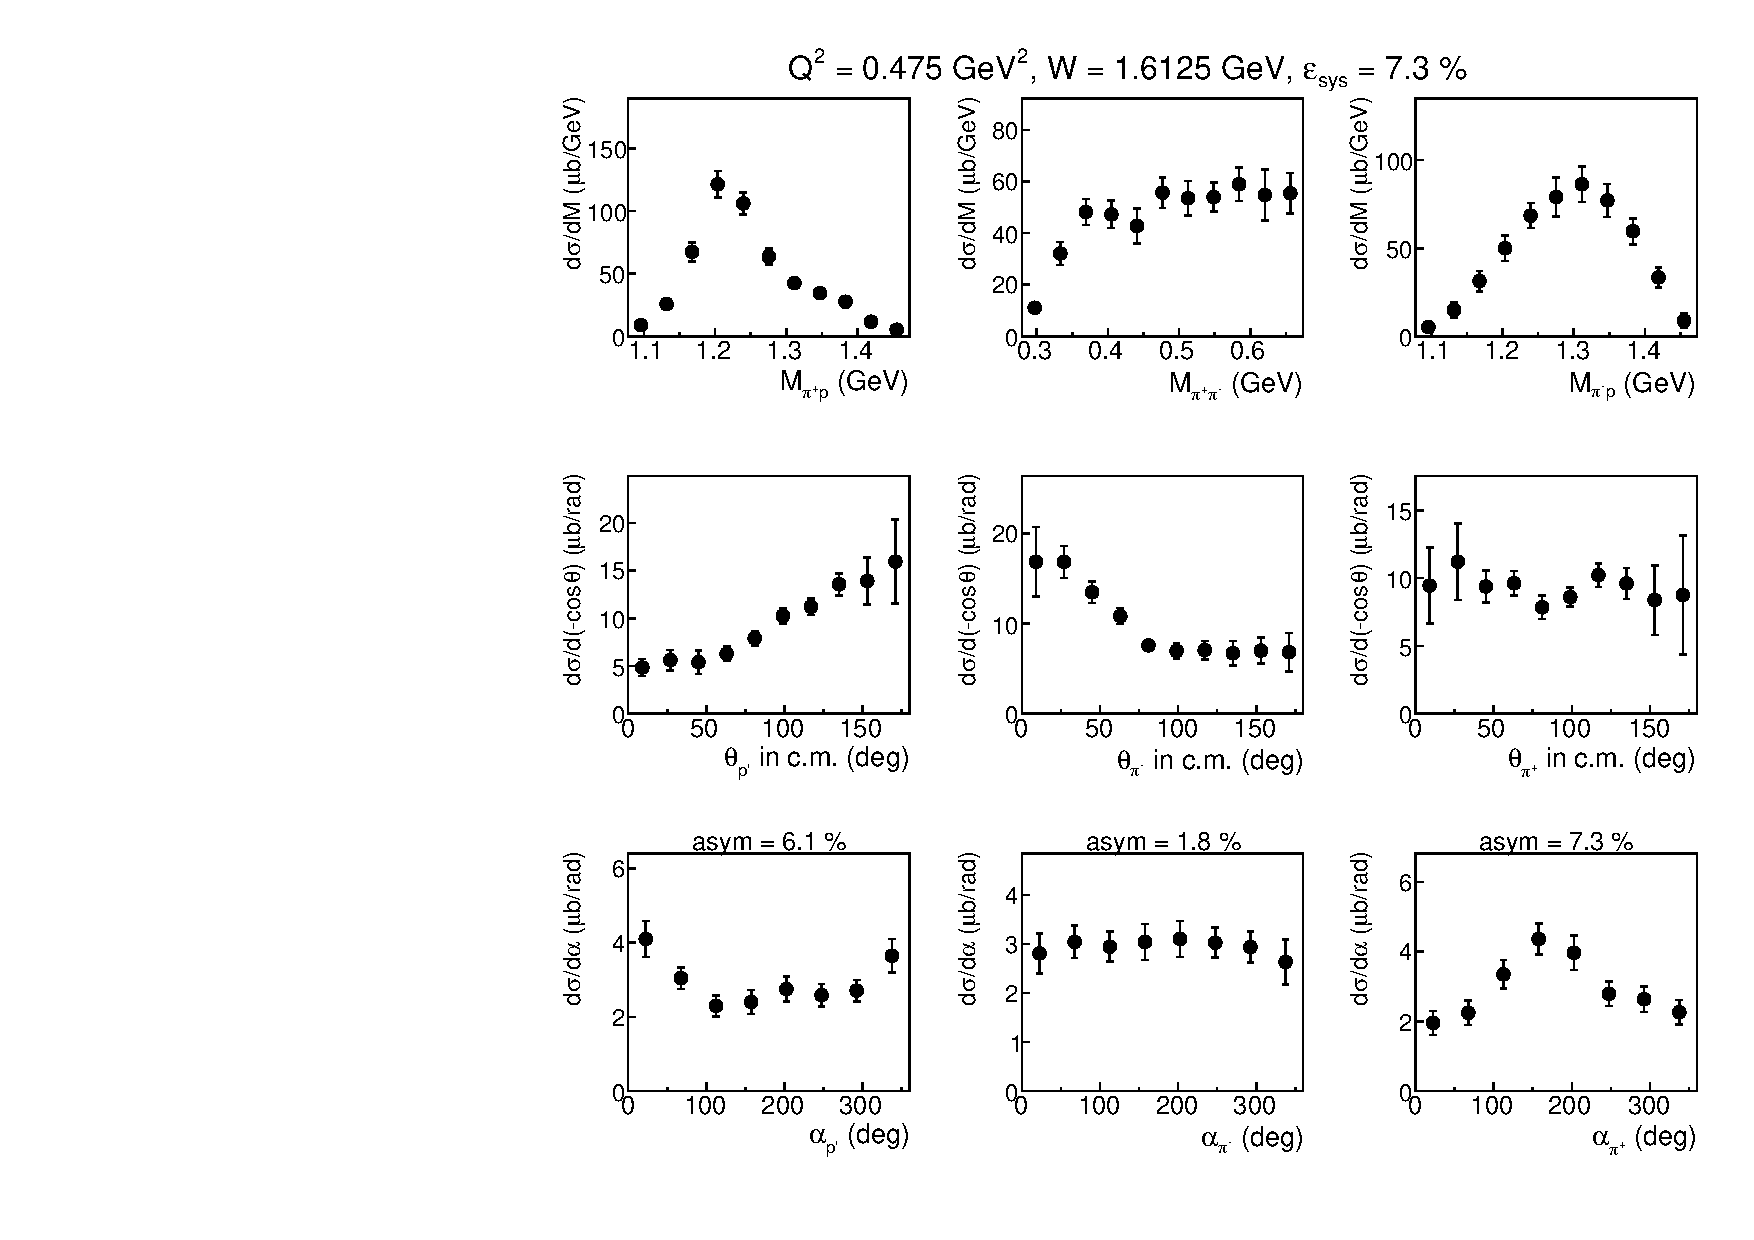
\includegraphics[width=0.495\textwidth]{pictures/appendix/1diff_distr/Q2_475/w_16125.pdf}}
\caption{\small Measured single-differential cross sections.} \label{fig:appx_4}
\end{center}
\end{figure}

\clearpage
\begin{figure}[htp]
\begin{center}
\frame{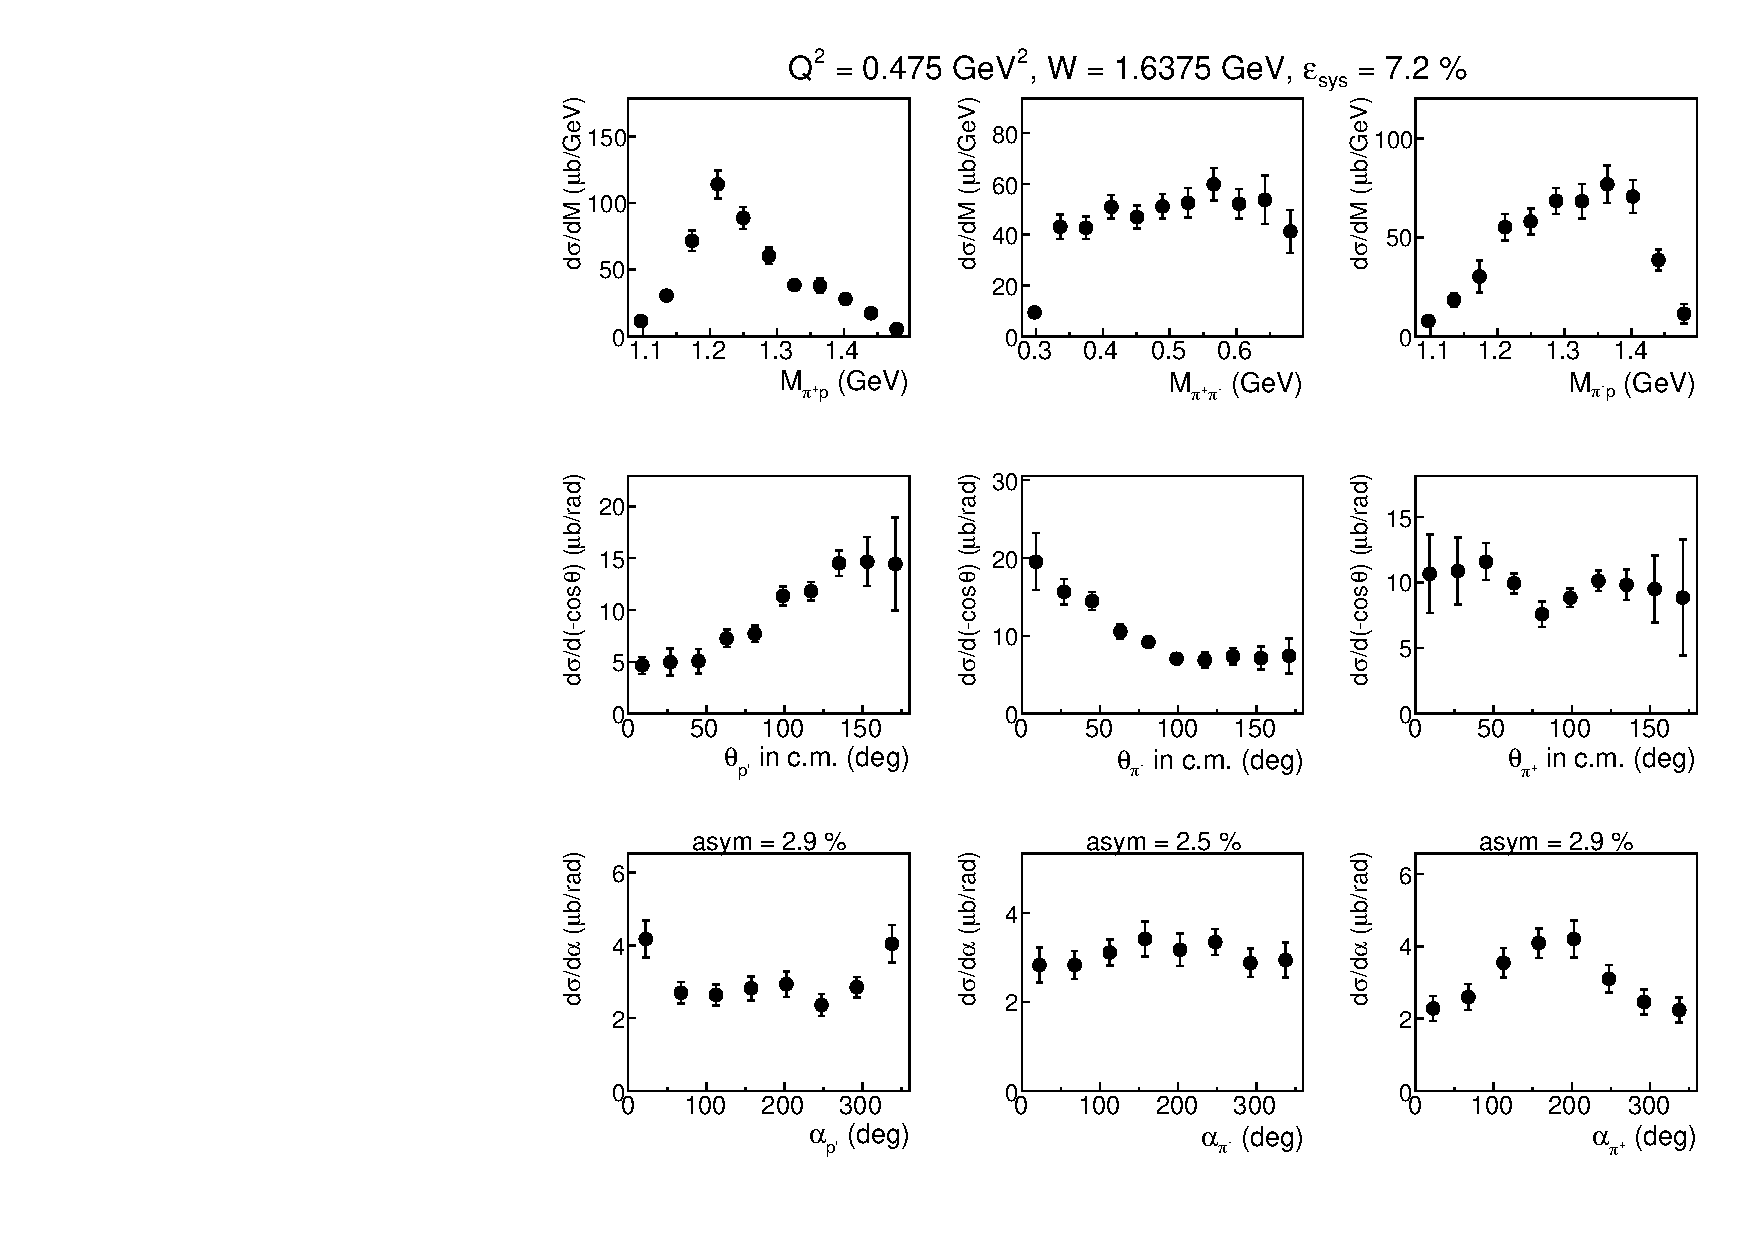
\includegraphics[width=0.495\textwidth]{pictures/appendix/1diff_distr/Q2_475/w_16375.pdf}}
\frame{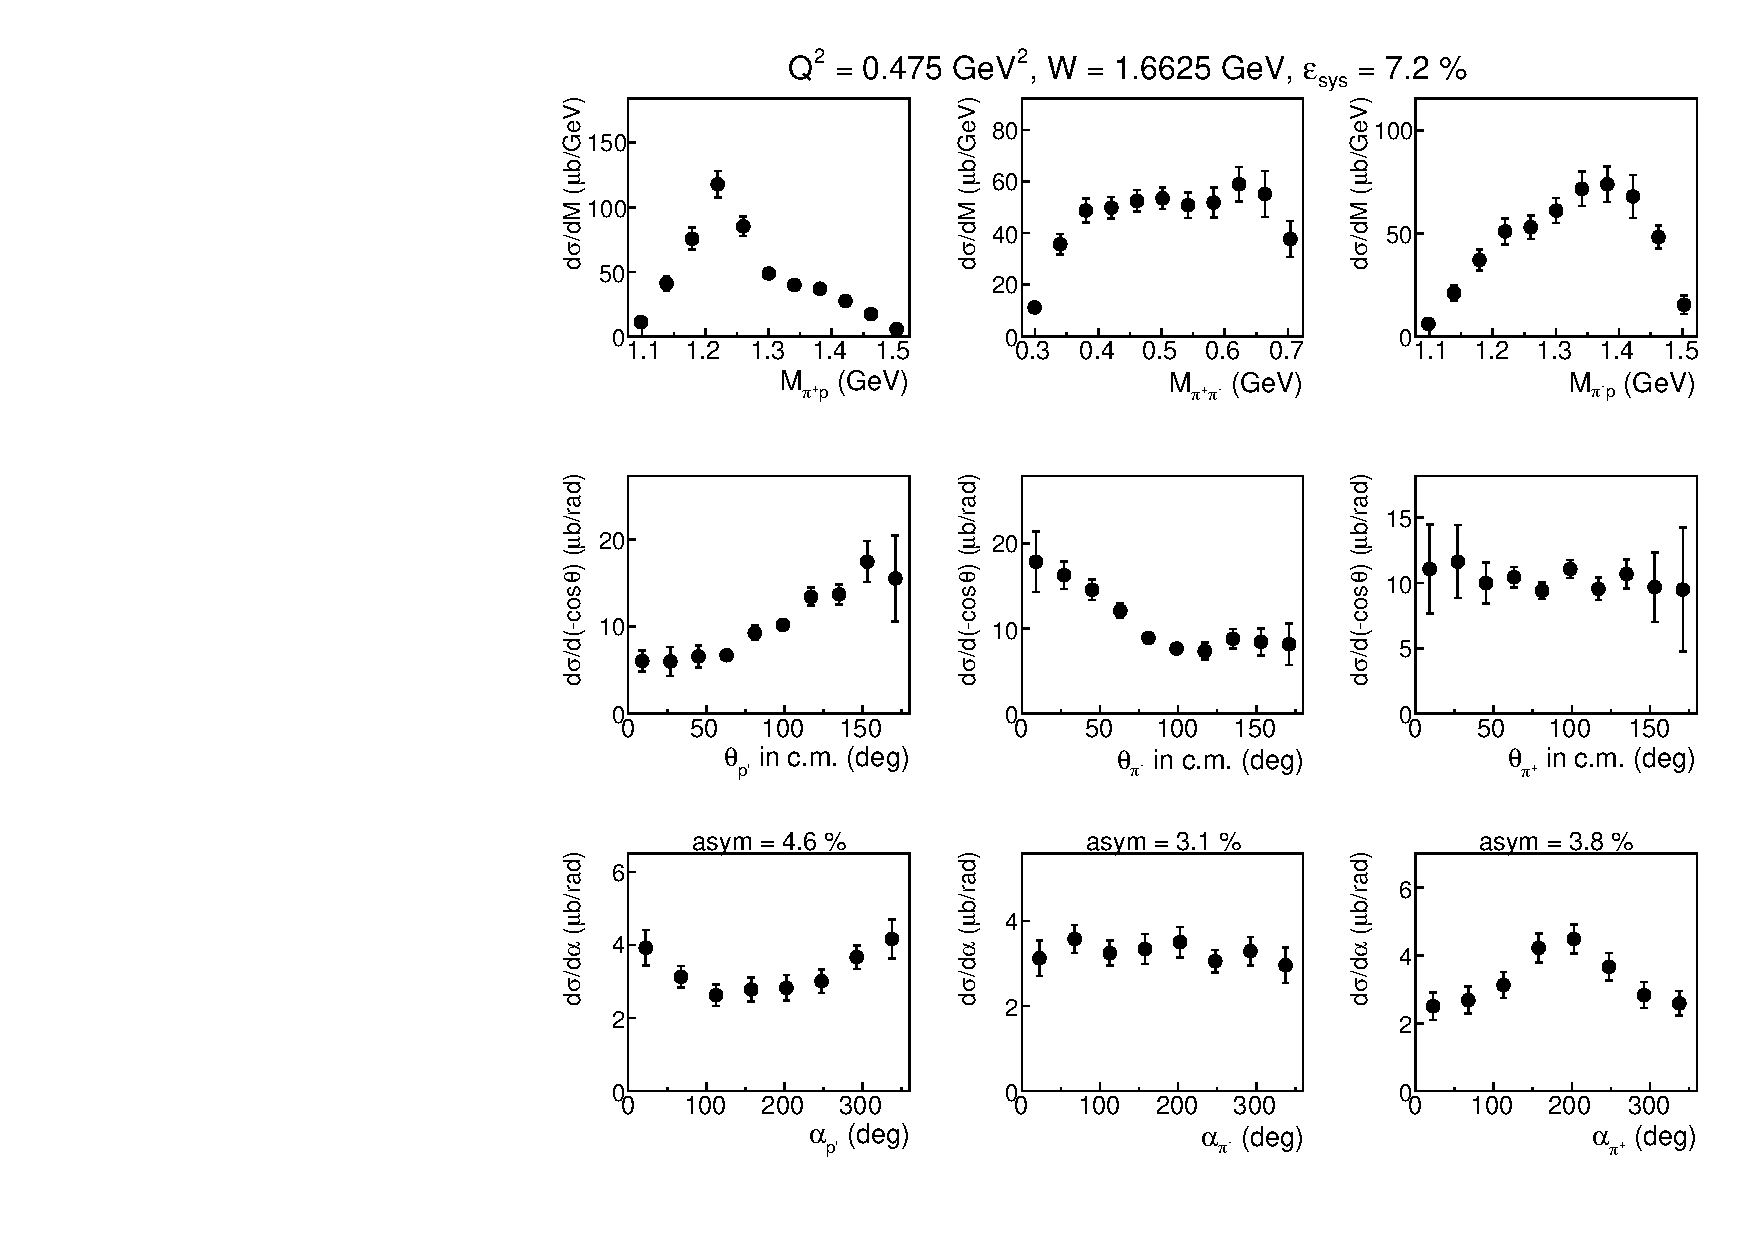
\includegraphics[width=0.495\textwidth]{pictures/appendix/1diff_distr/Q2_475/w_16625.pdf}}
\frame{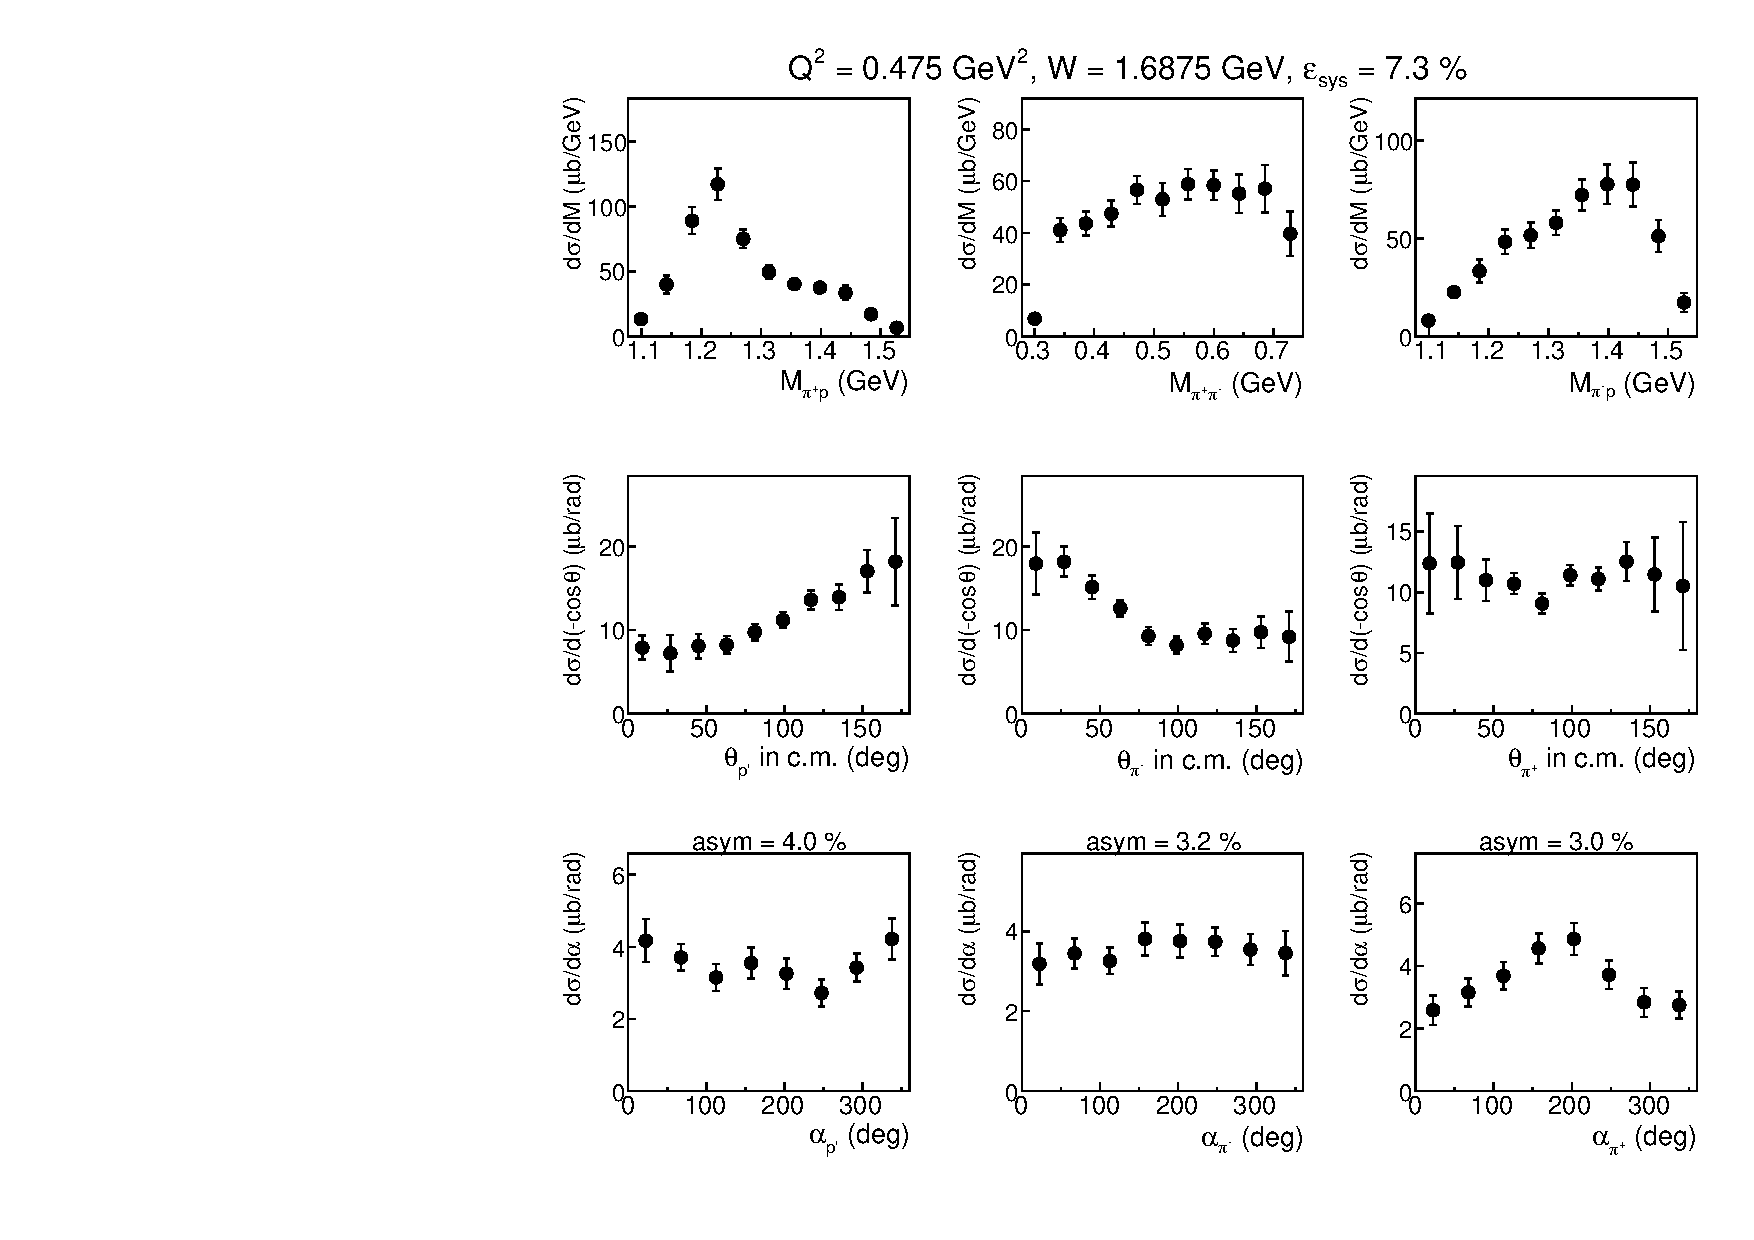
\includegraphics[width=0.495\textwidth]{pictures/appendix/1diff_distr/Q2_475/w_16875.pdf}}
\frame{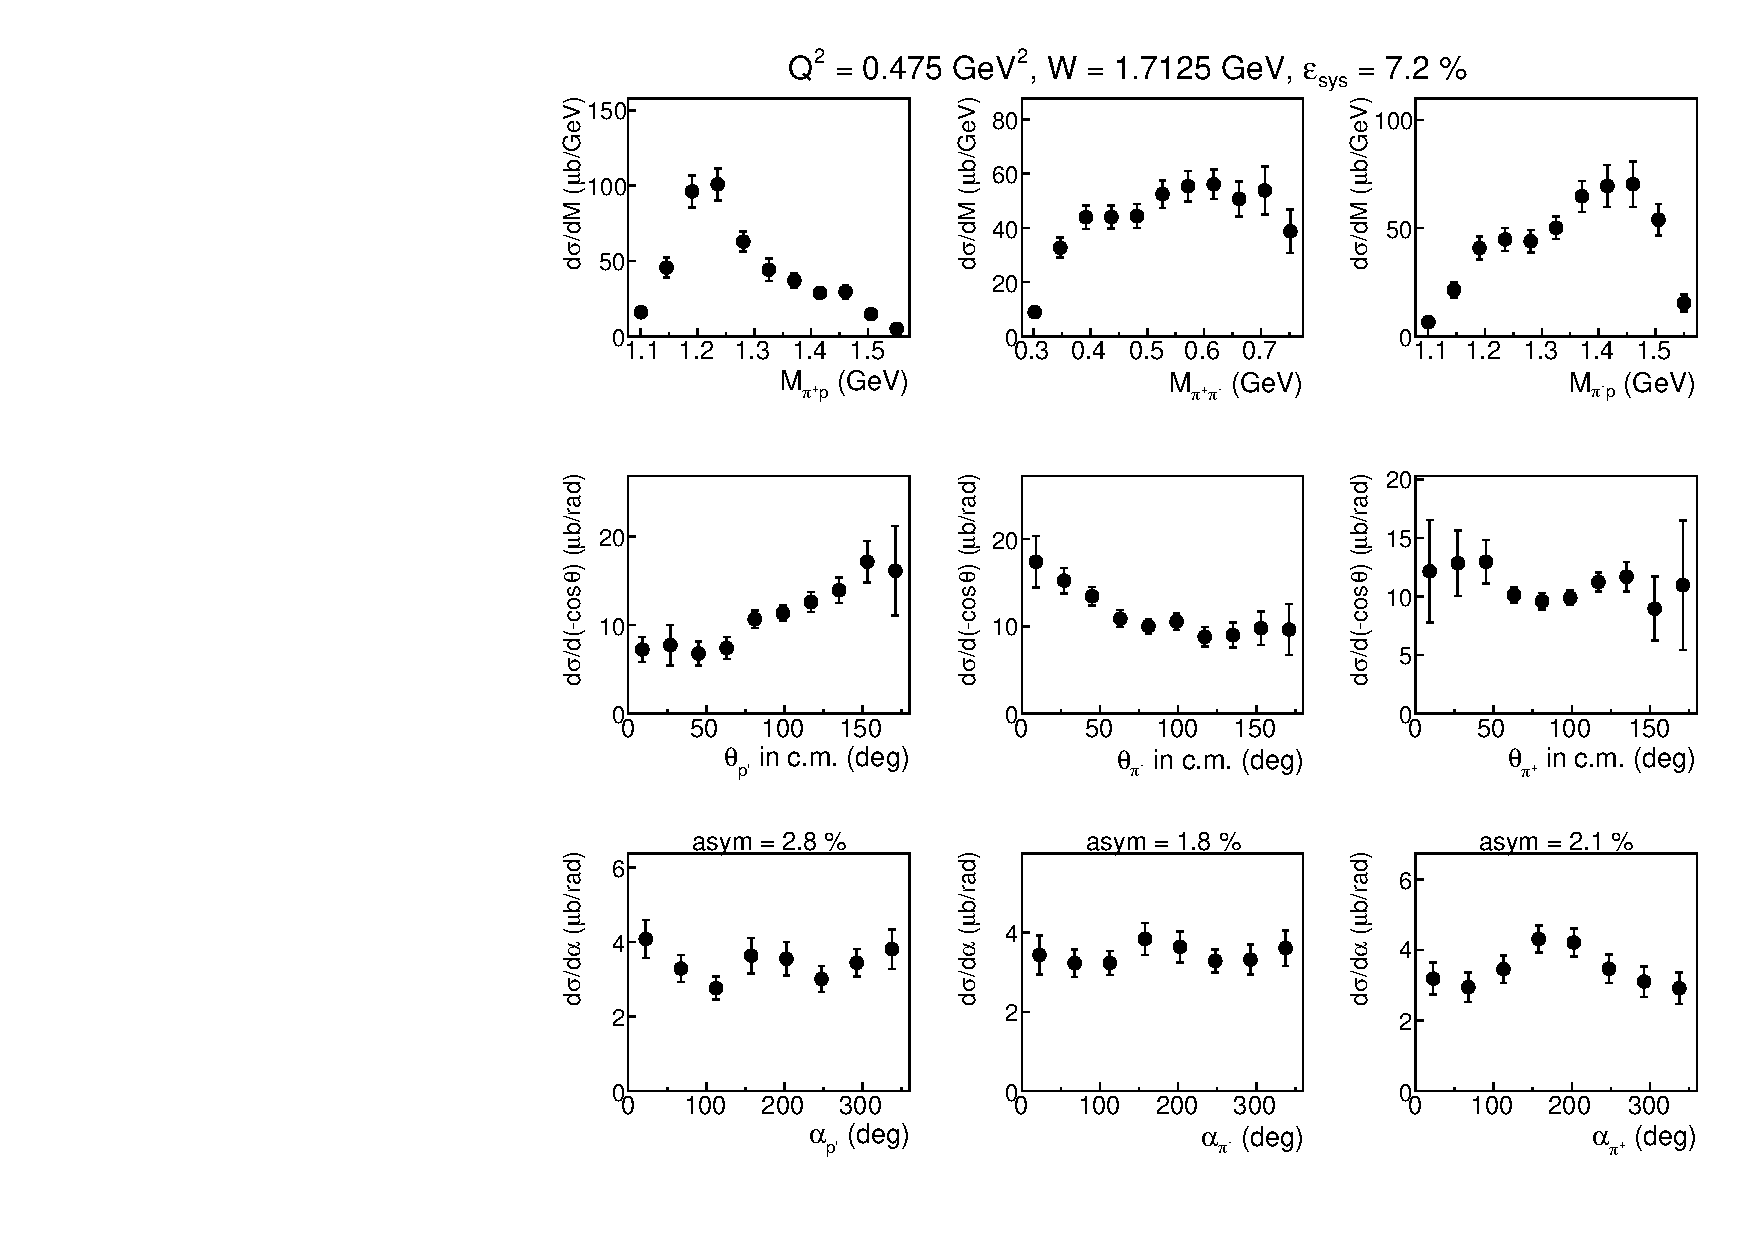
\includegraphics[width=0.495\textwidth]{pictures/appendix/1diff_distr/Q2_475/w_17125.pdf}}
\frame{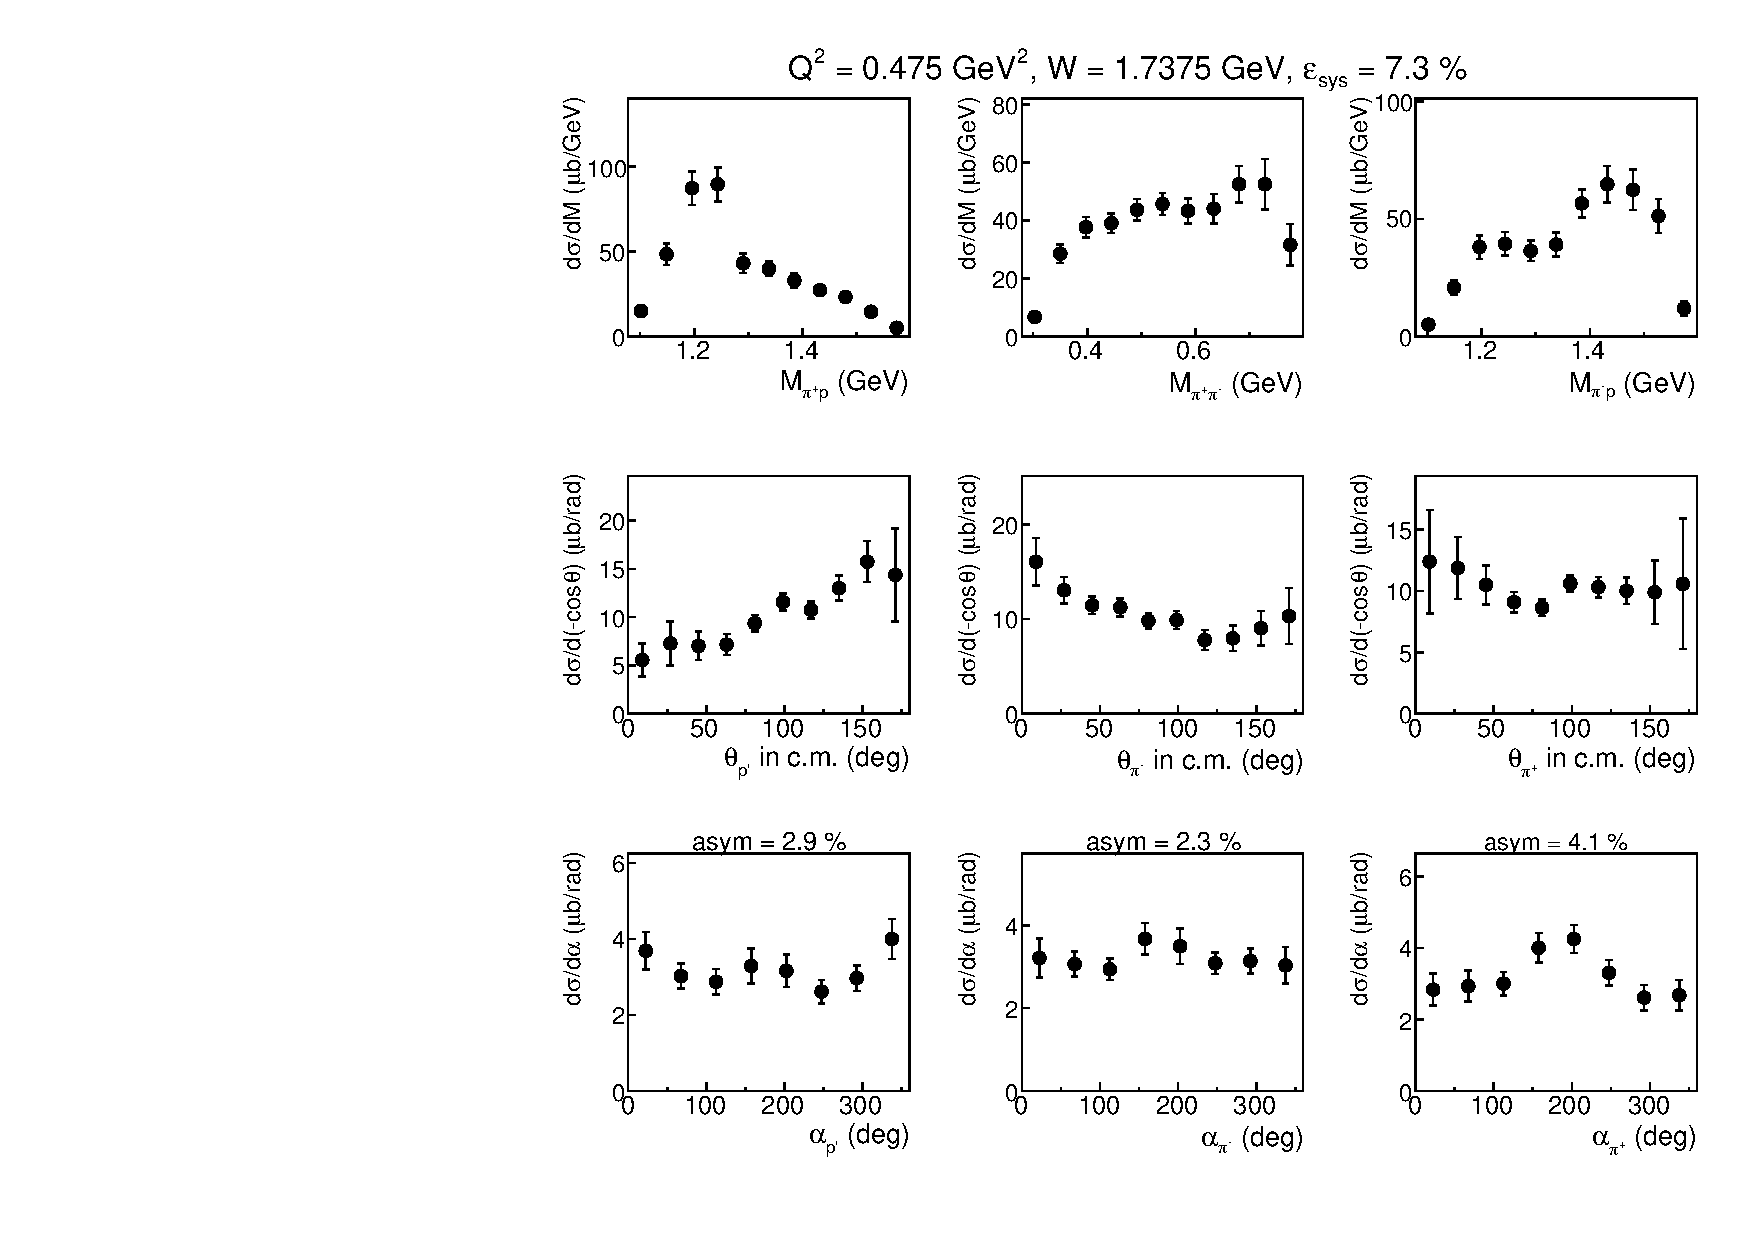
\includegraphics[width=0.495\textwidth]{pictures/appendix/1diff_distr/Q2_475/w_17375.pdf}}
\frame{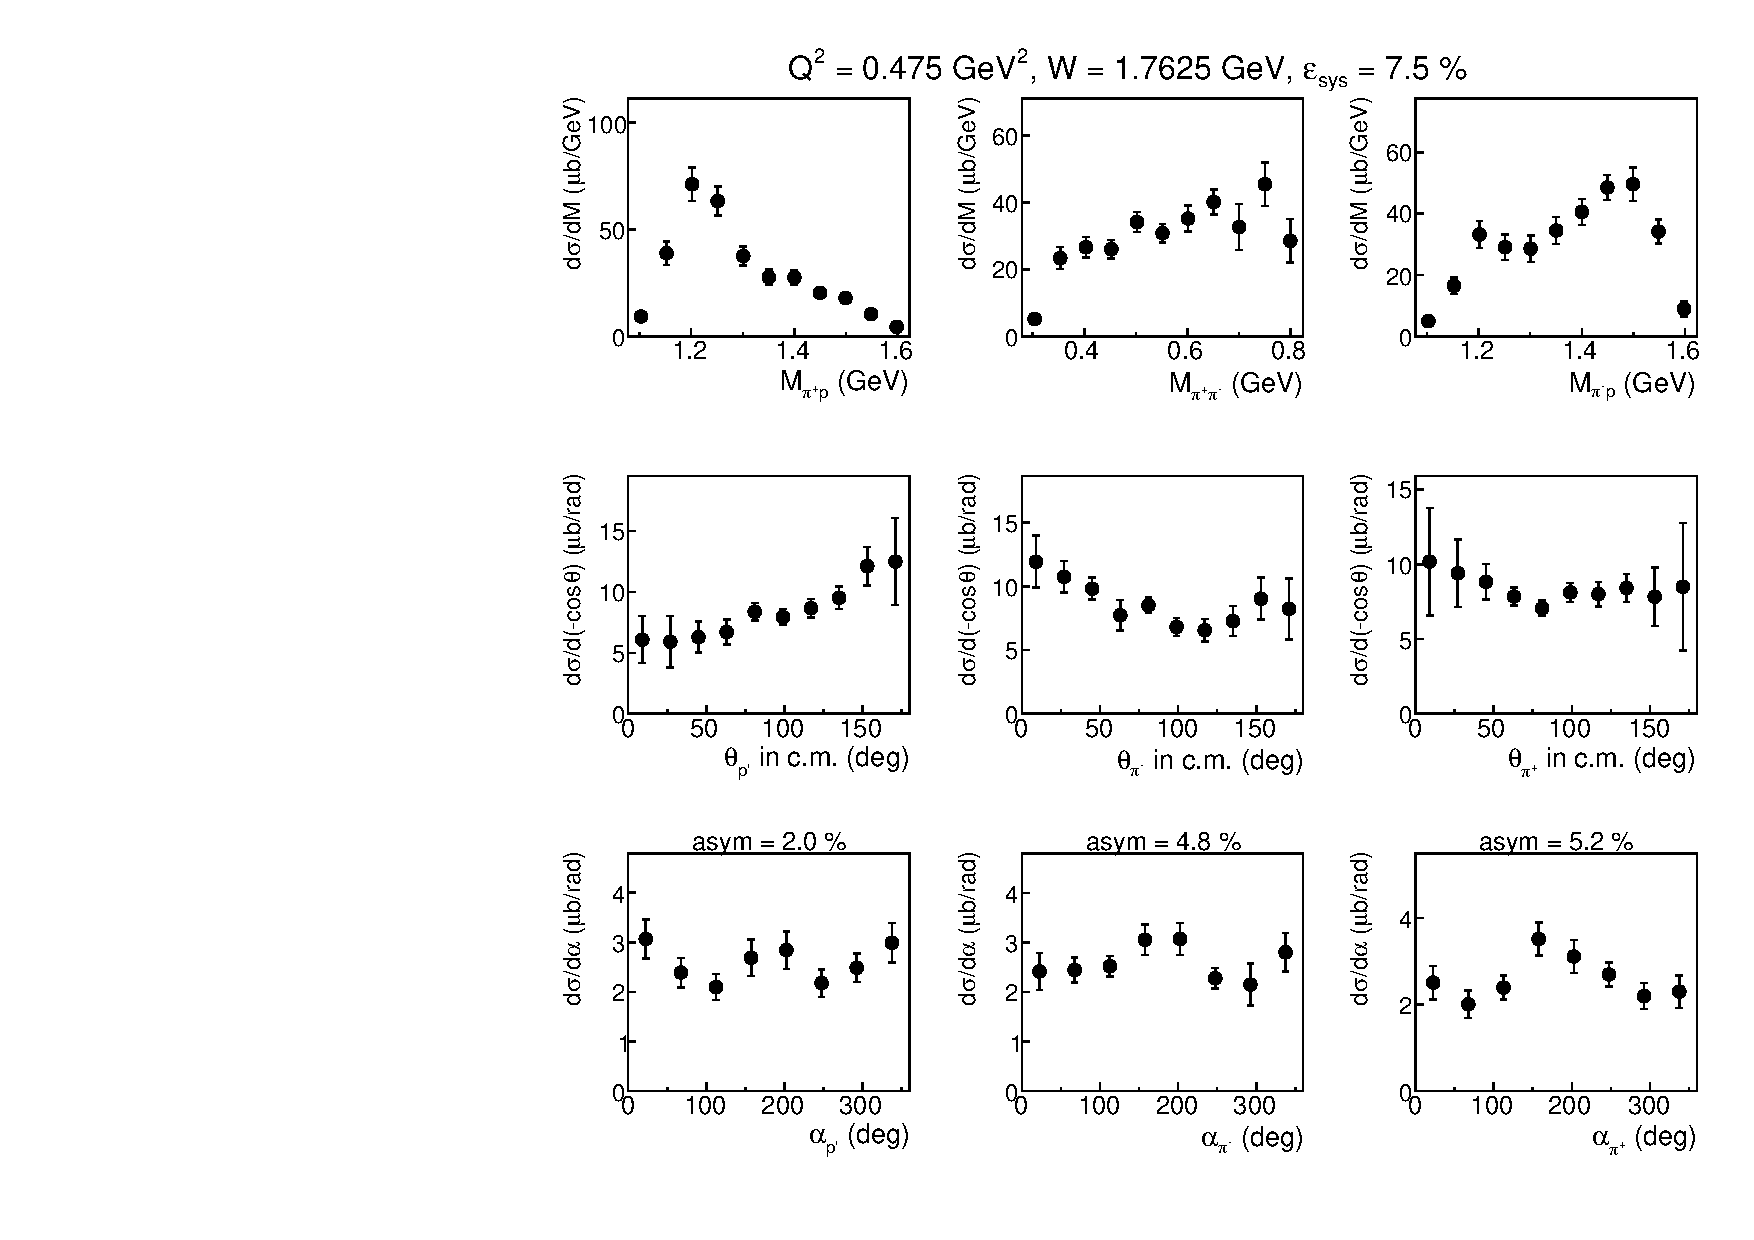
\includegraphics[width=0.495\textwidth]{pictures/appendix/1diff_distr/Q2_475/w_17625.pdf}}
\caption{\small Measured single-differential cross sections.} \label{fig:appx_5}
\end{center}
\end{figure}

\clearpage
\begin{figure}[htp]
\begin{center}
\frame{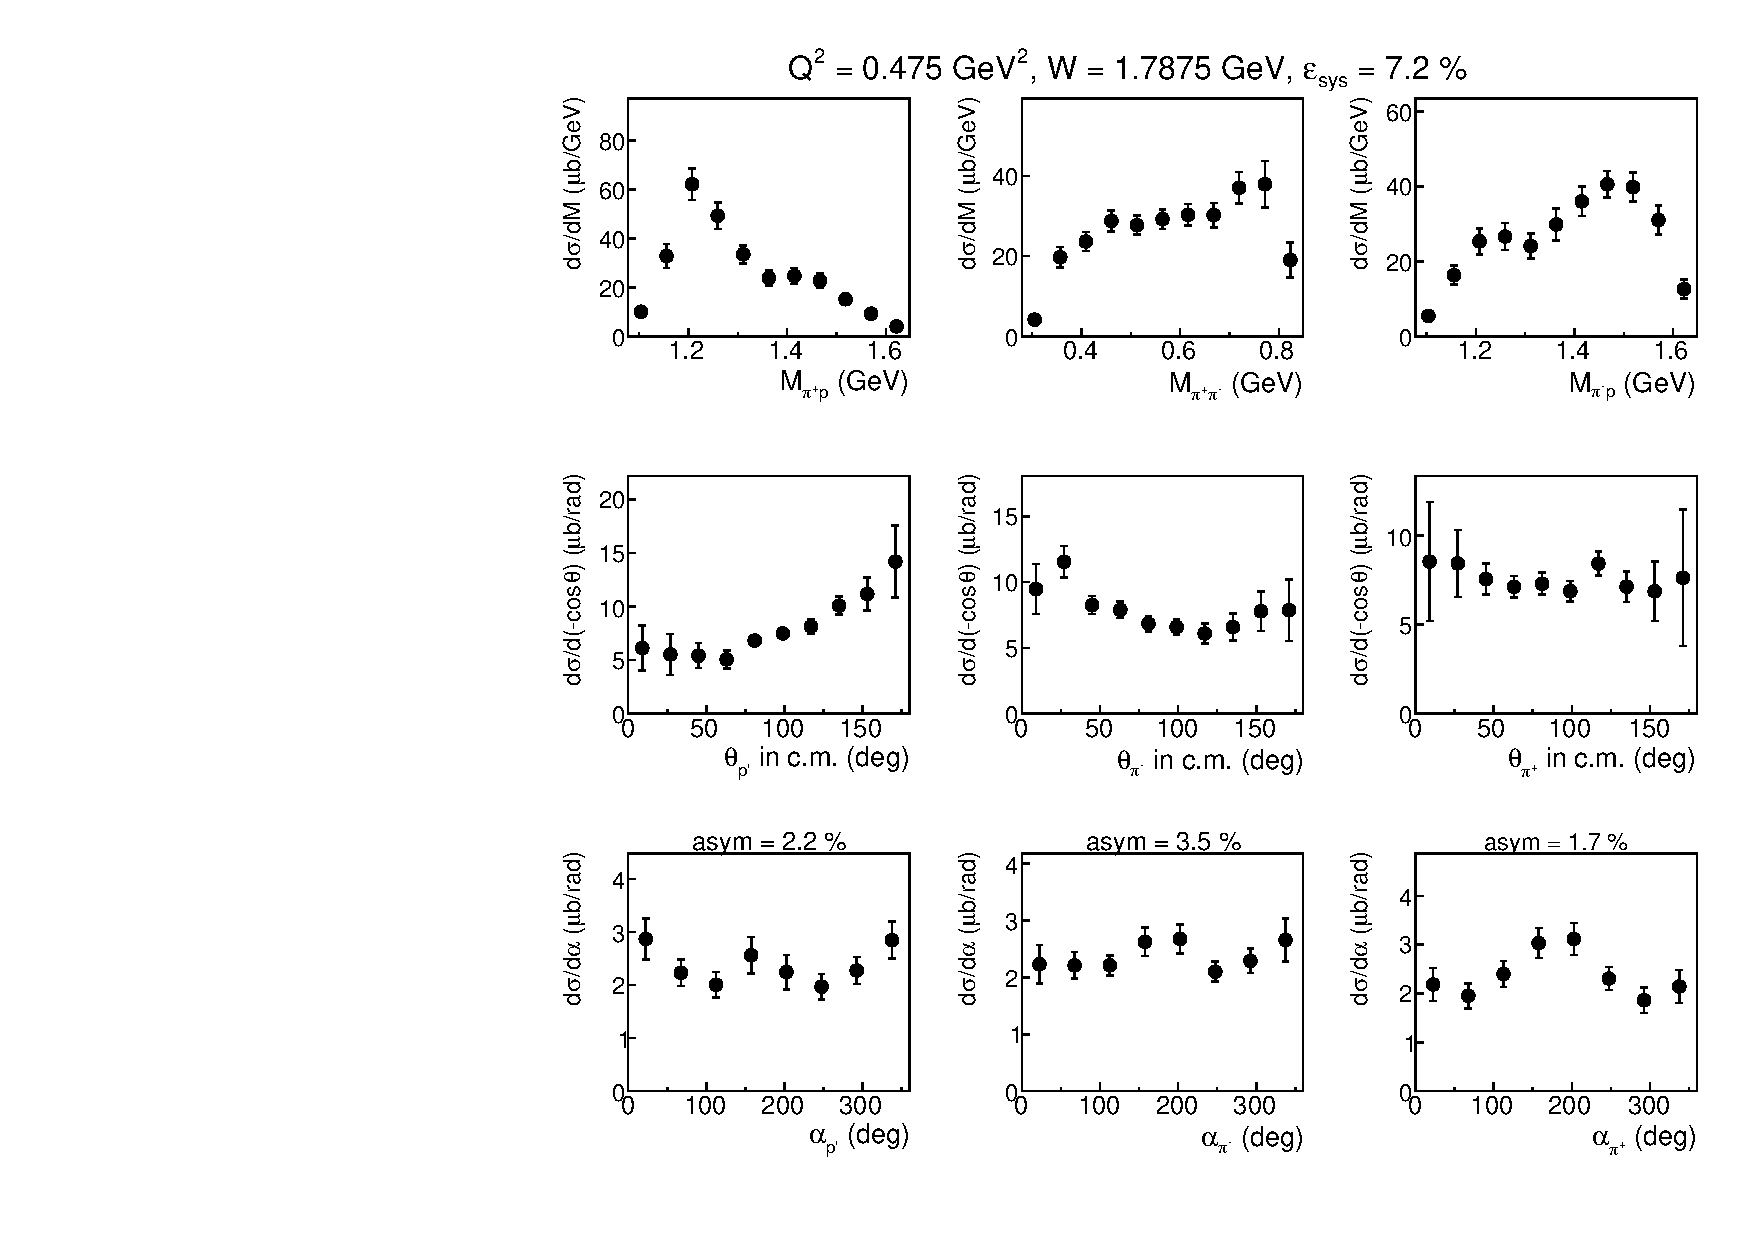
\includegraphics[width=0.495\textwidth]{pictures/appendix/1diff_distr/Q2_475/w_17875.pdf}}
\frame{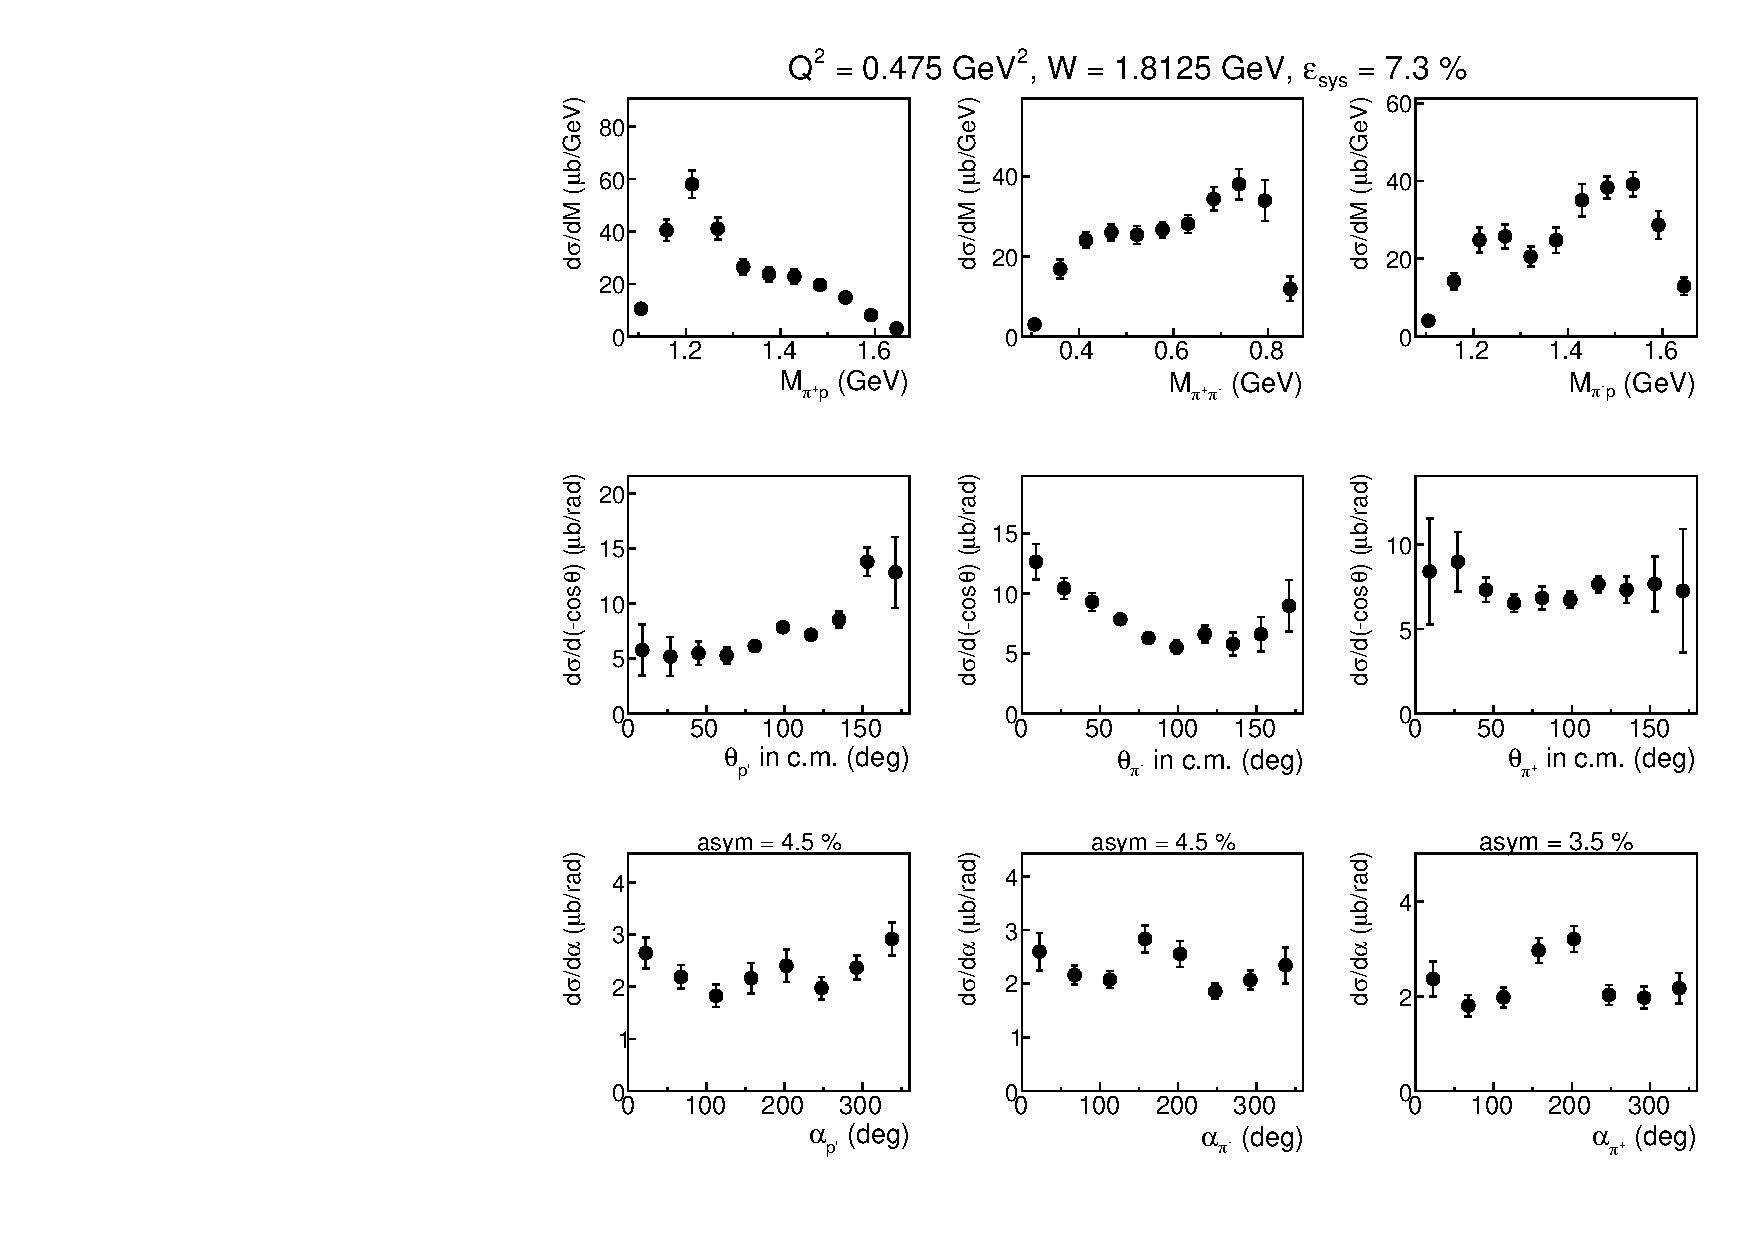
\includegraphics[width=0.495\textwidth]{pictures/appendix/1diff_distr/Q2_475/w_18125.pdf}}
\frame{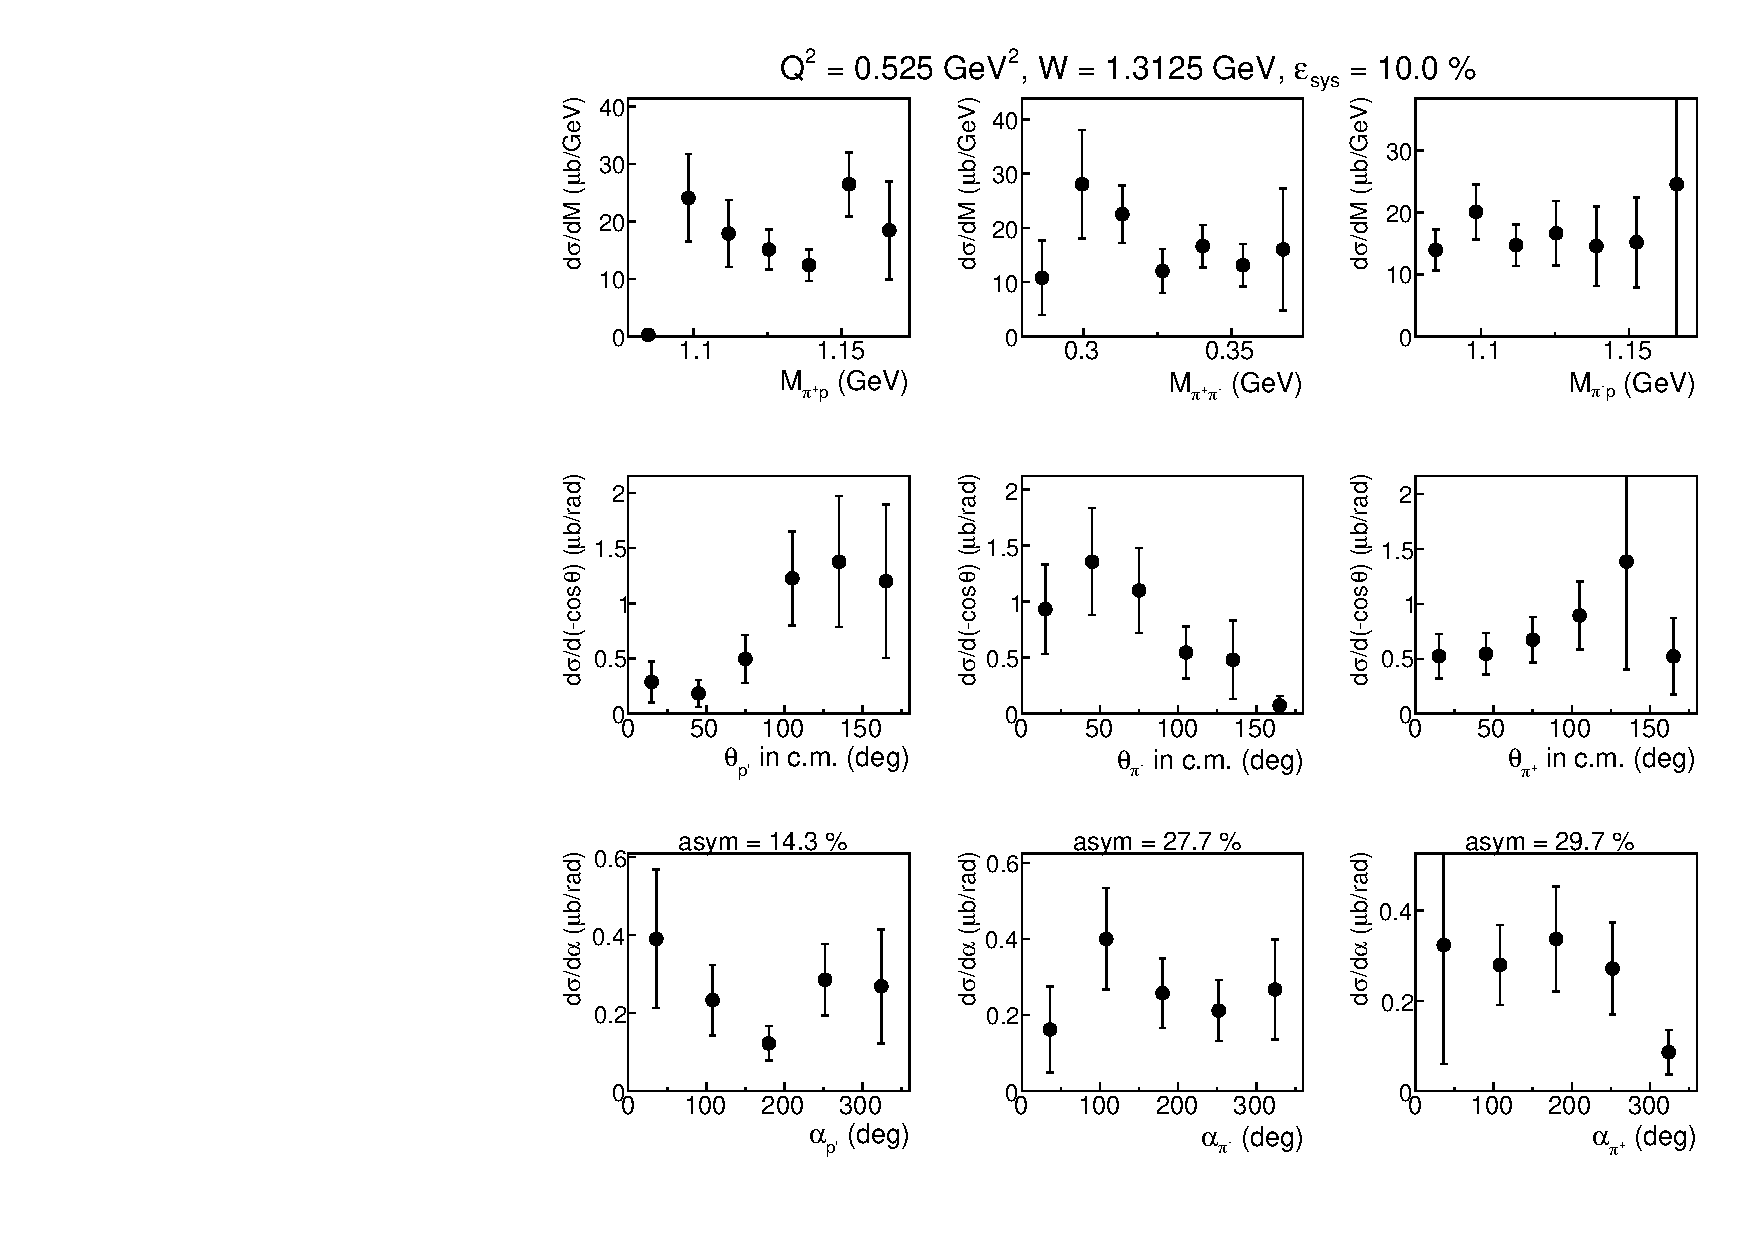
\includegraphics[width=0.495\textwidth]{pictures/appendix/1diff_distr/Q2_525/w_13125.pdf}}
\frame{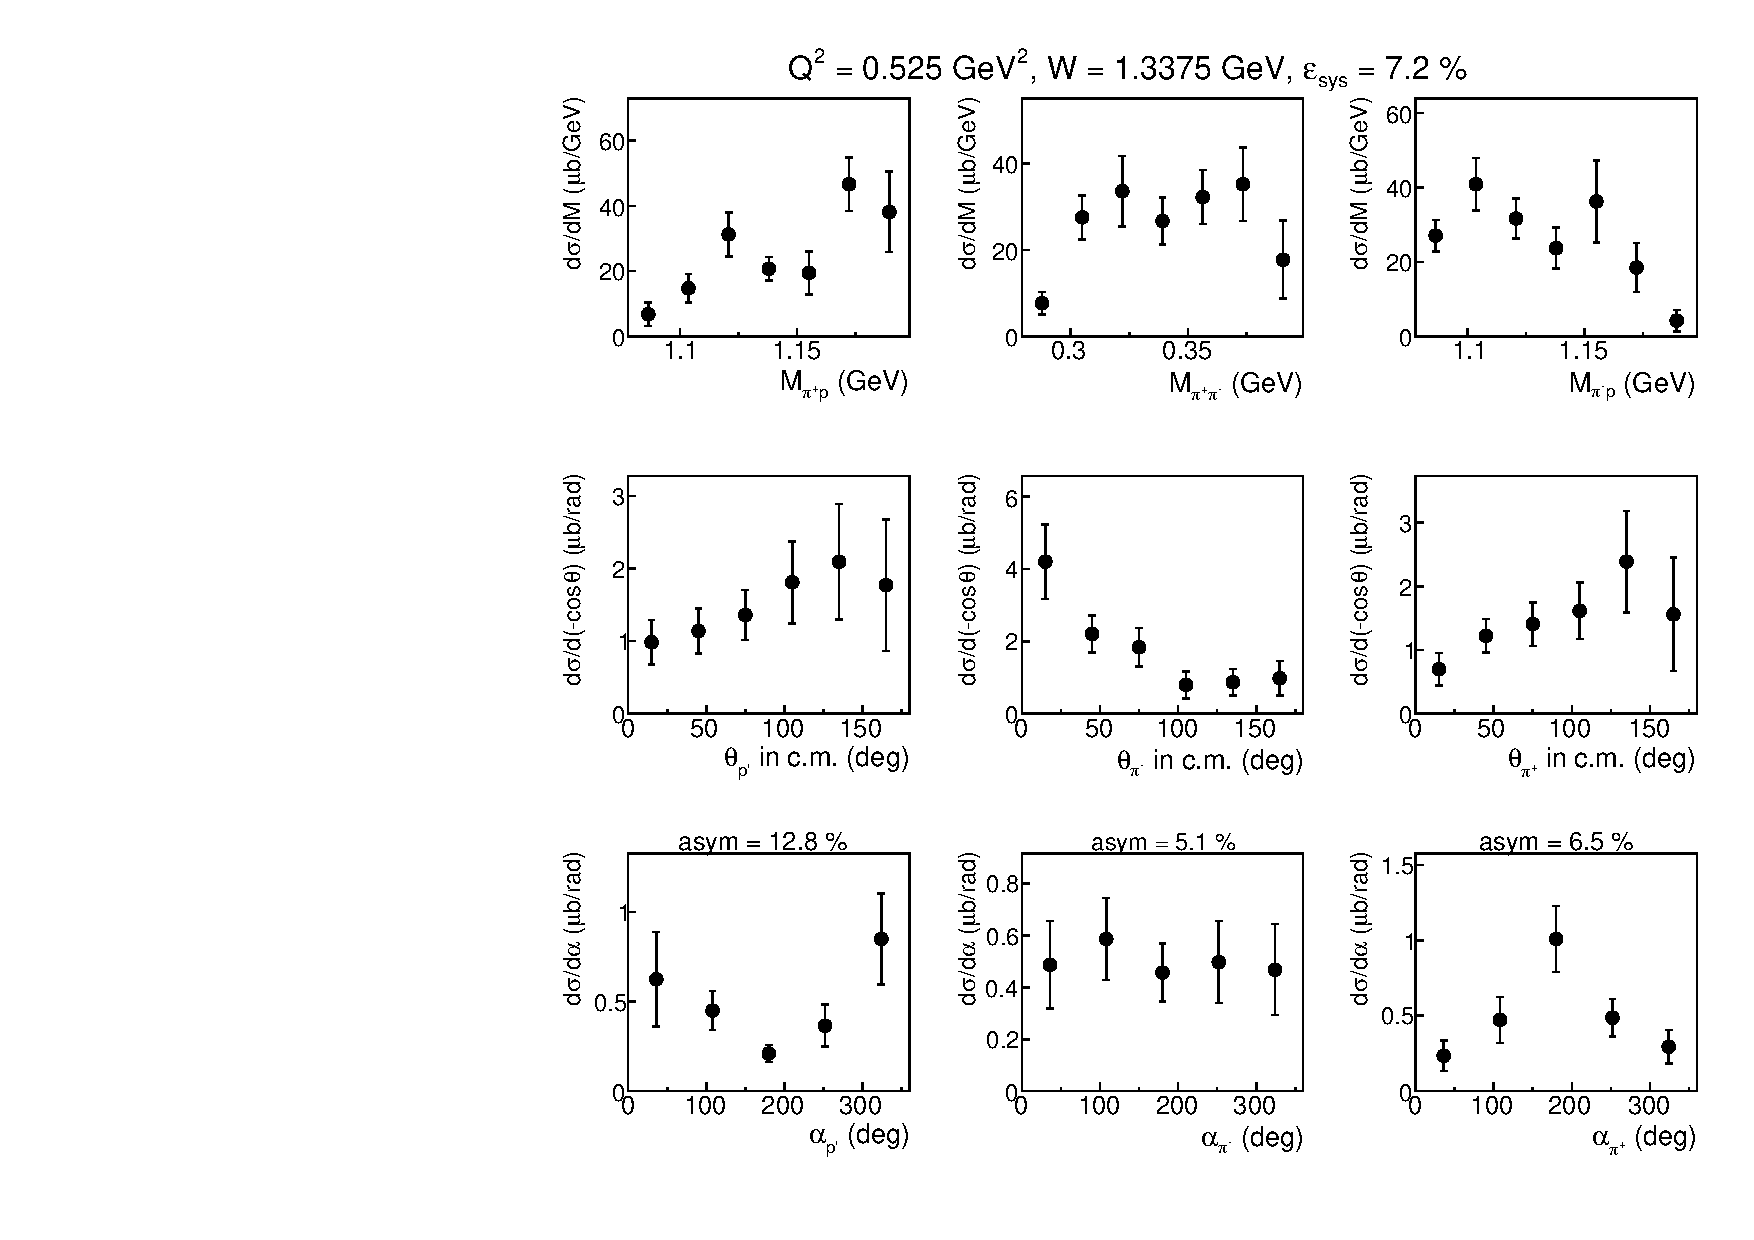
\includegraphics[width=0.495\textwidth]{pictures/appendix/1diff_distr/Q2_525/w_13375.pdf}}
\frame{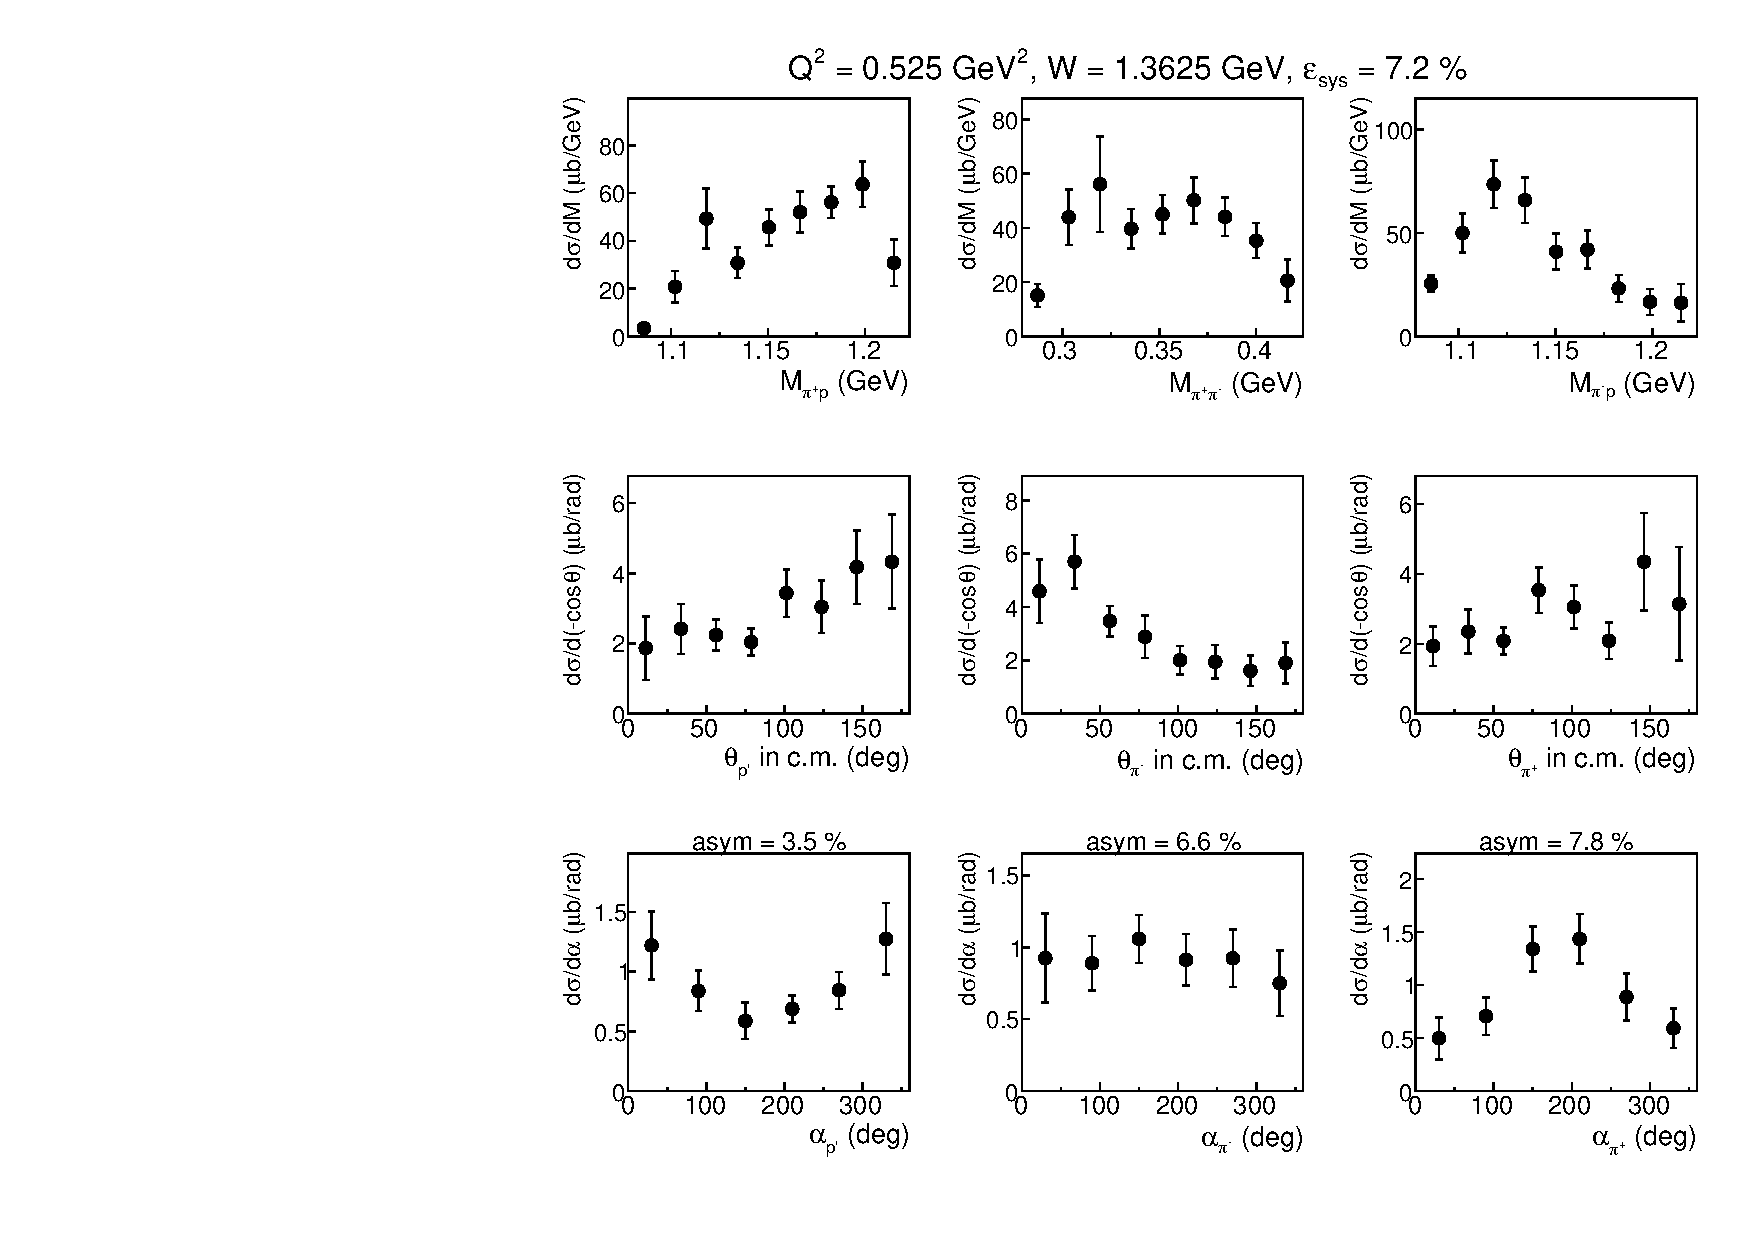
\includegraphics[width=0.495\textwidth]{pictures/appendix/1diff_distr/Q2_525/w_13625.pdf}}
\frame{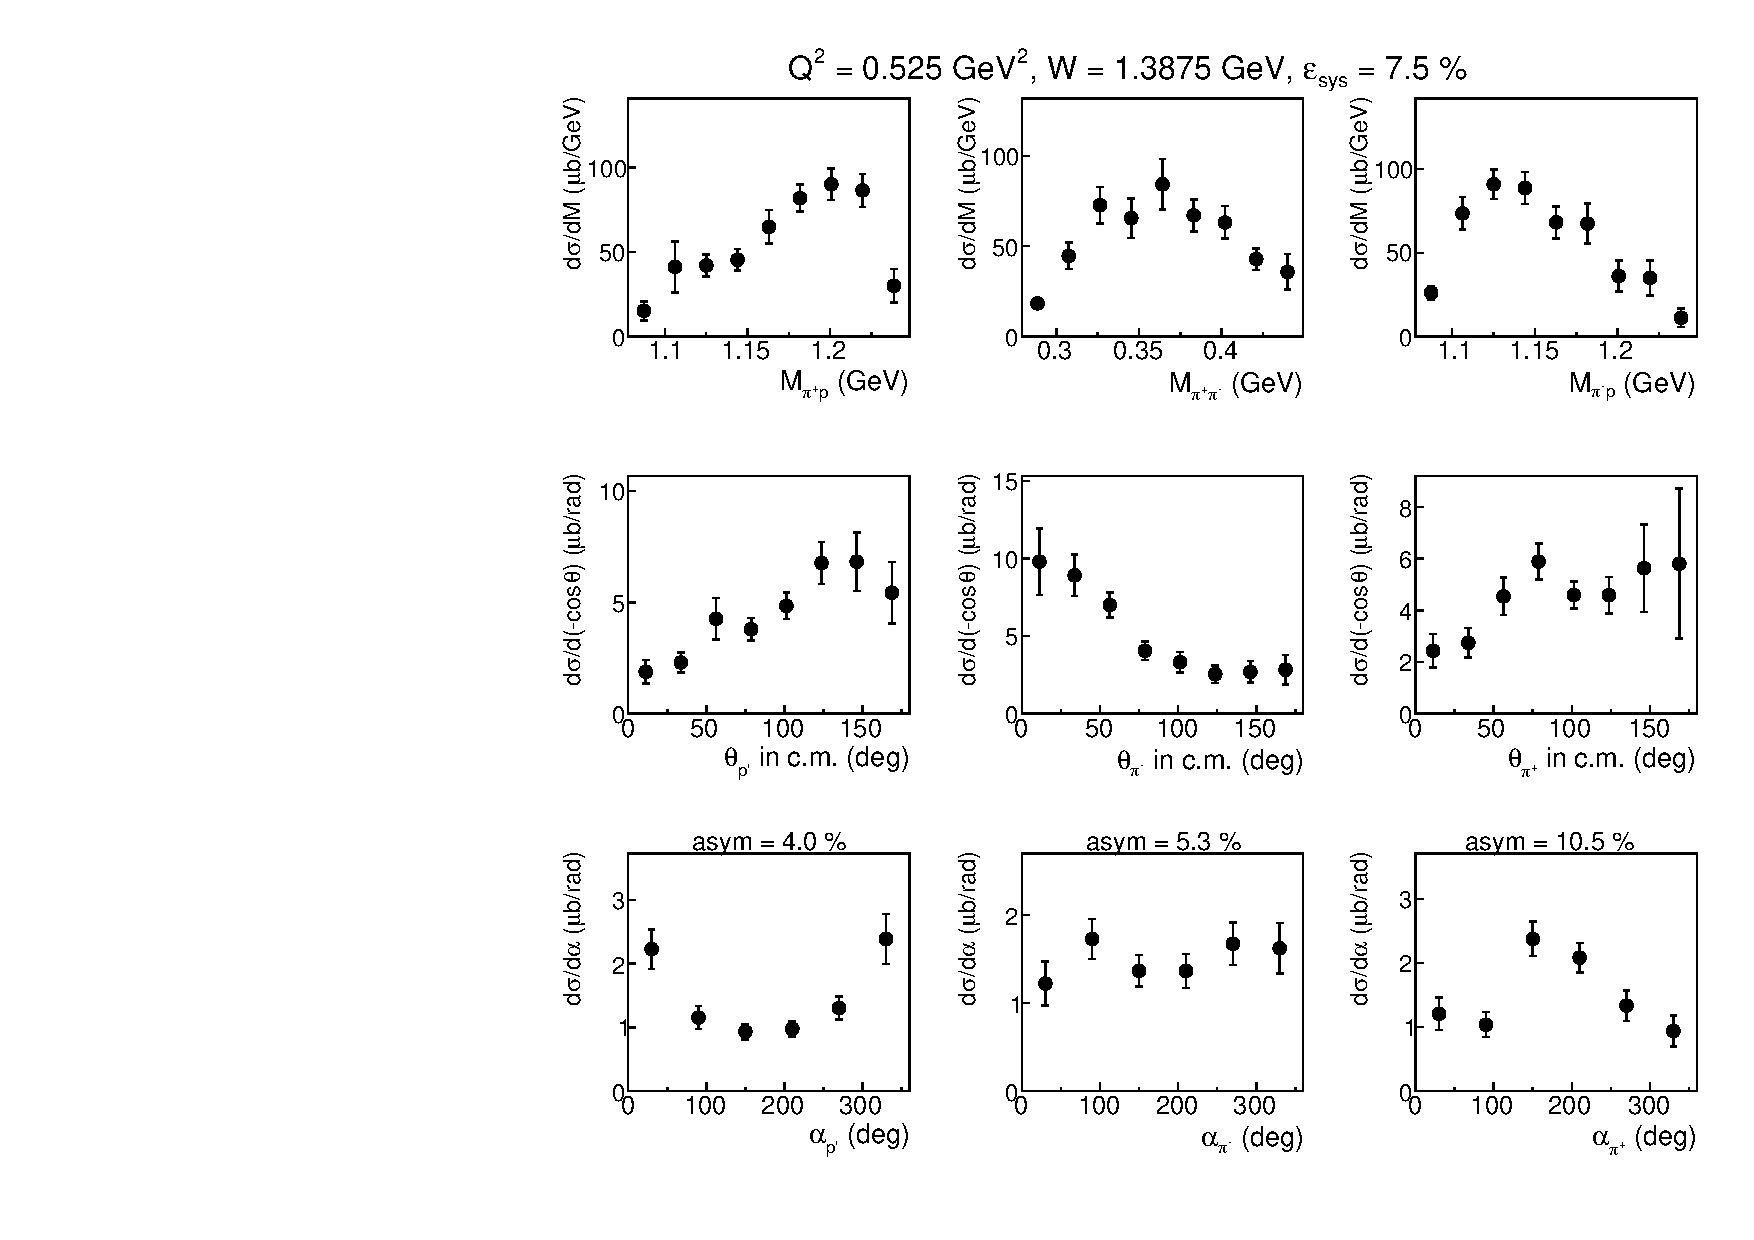
\includegraphics[width=0.495\textwidth]{pictures/appendix/1diff_distr/Q2_525/w_13875.pdf}}
\caption{\small Measured single-differential cross sections.} \label{fig:appx_6}
\end{center}
\end{figure}

\clearpage
\begin{figure}[htp]
\begin{center}
\frame{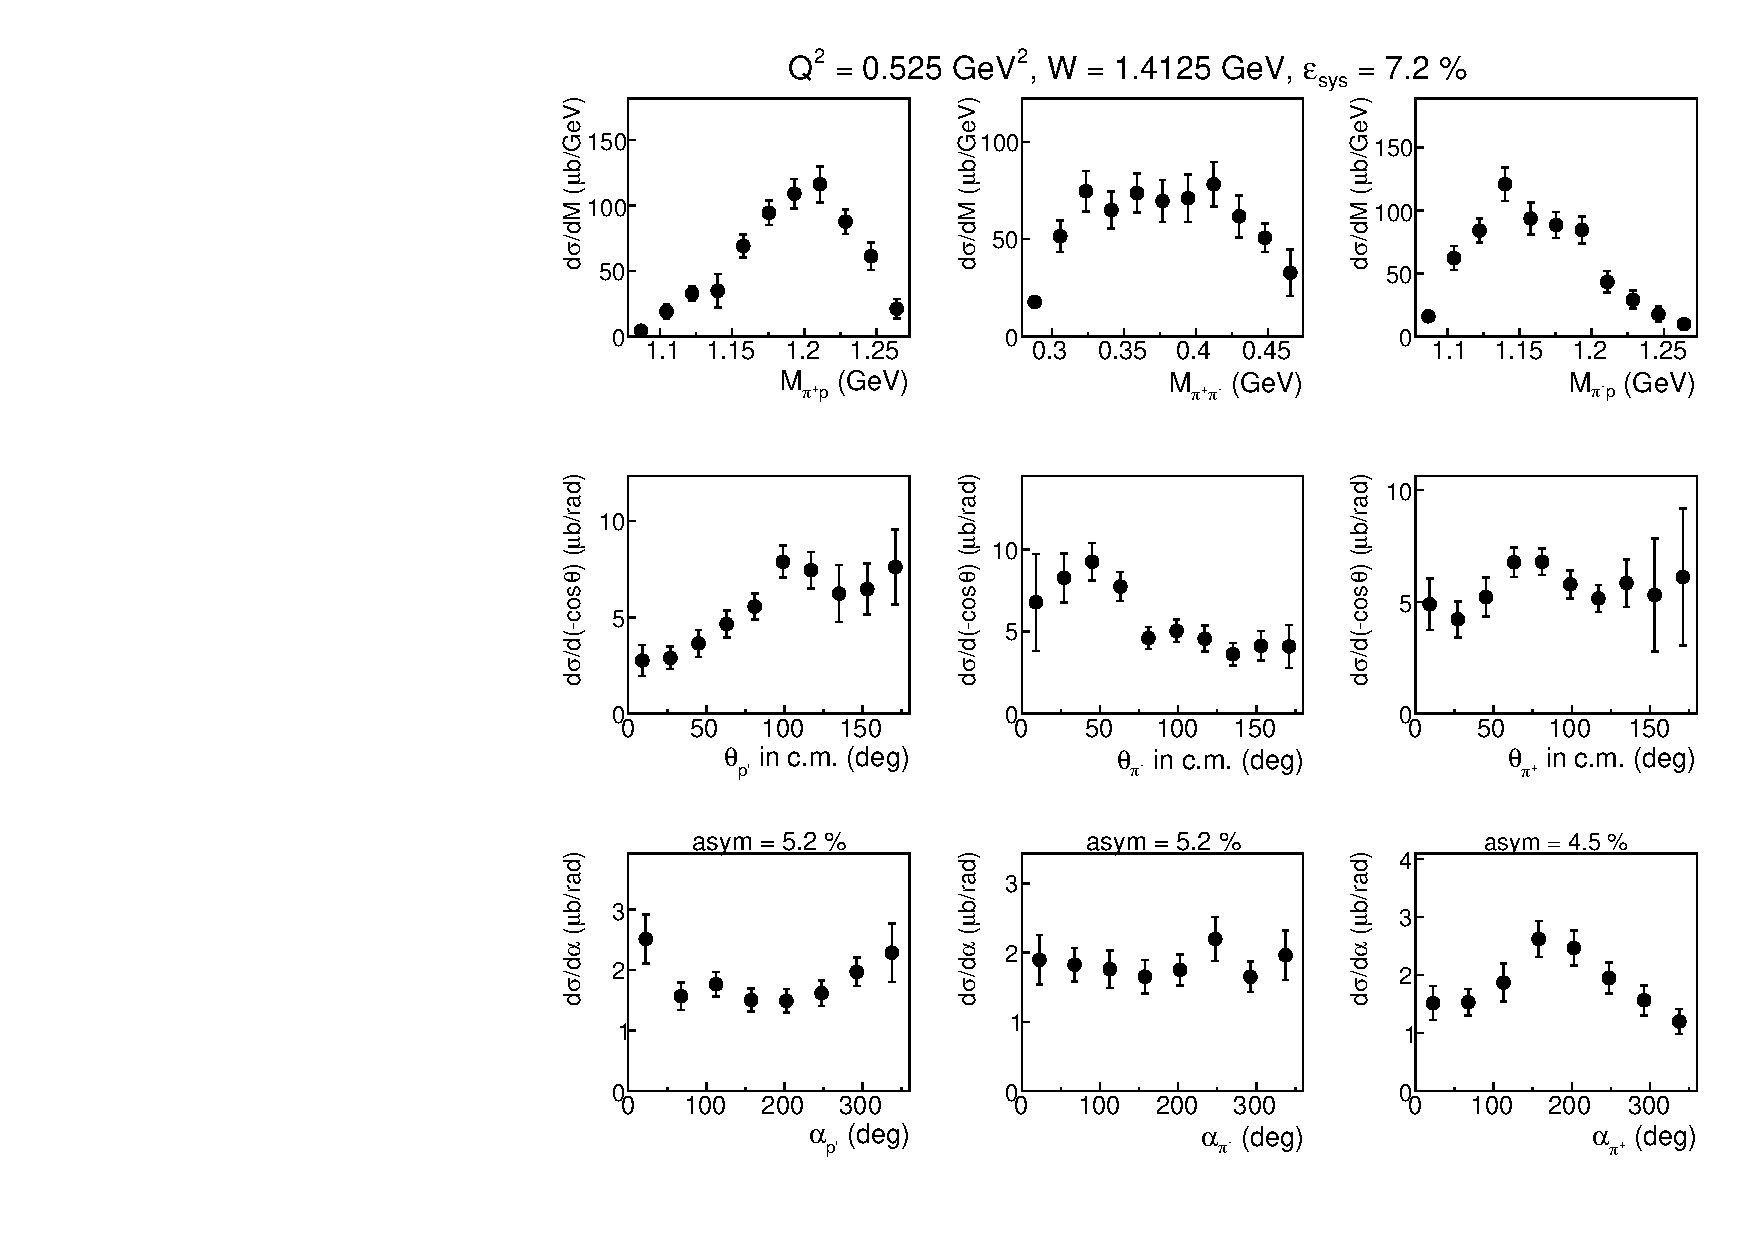
\includegraphics[width=0.495\textwidth]{pictures/appendix/1diff_distr/Q2_525/w_14125.pdf}}
\frame{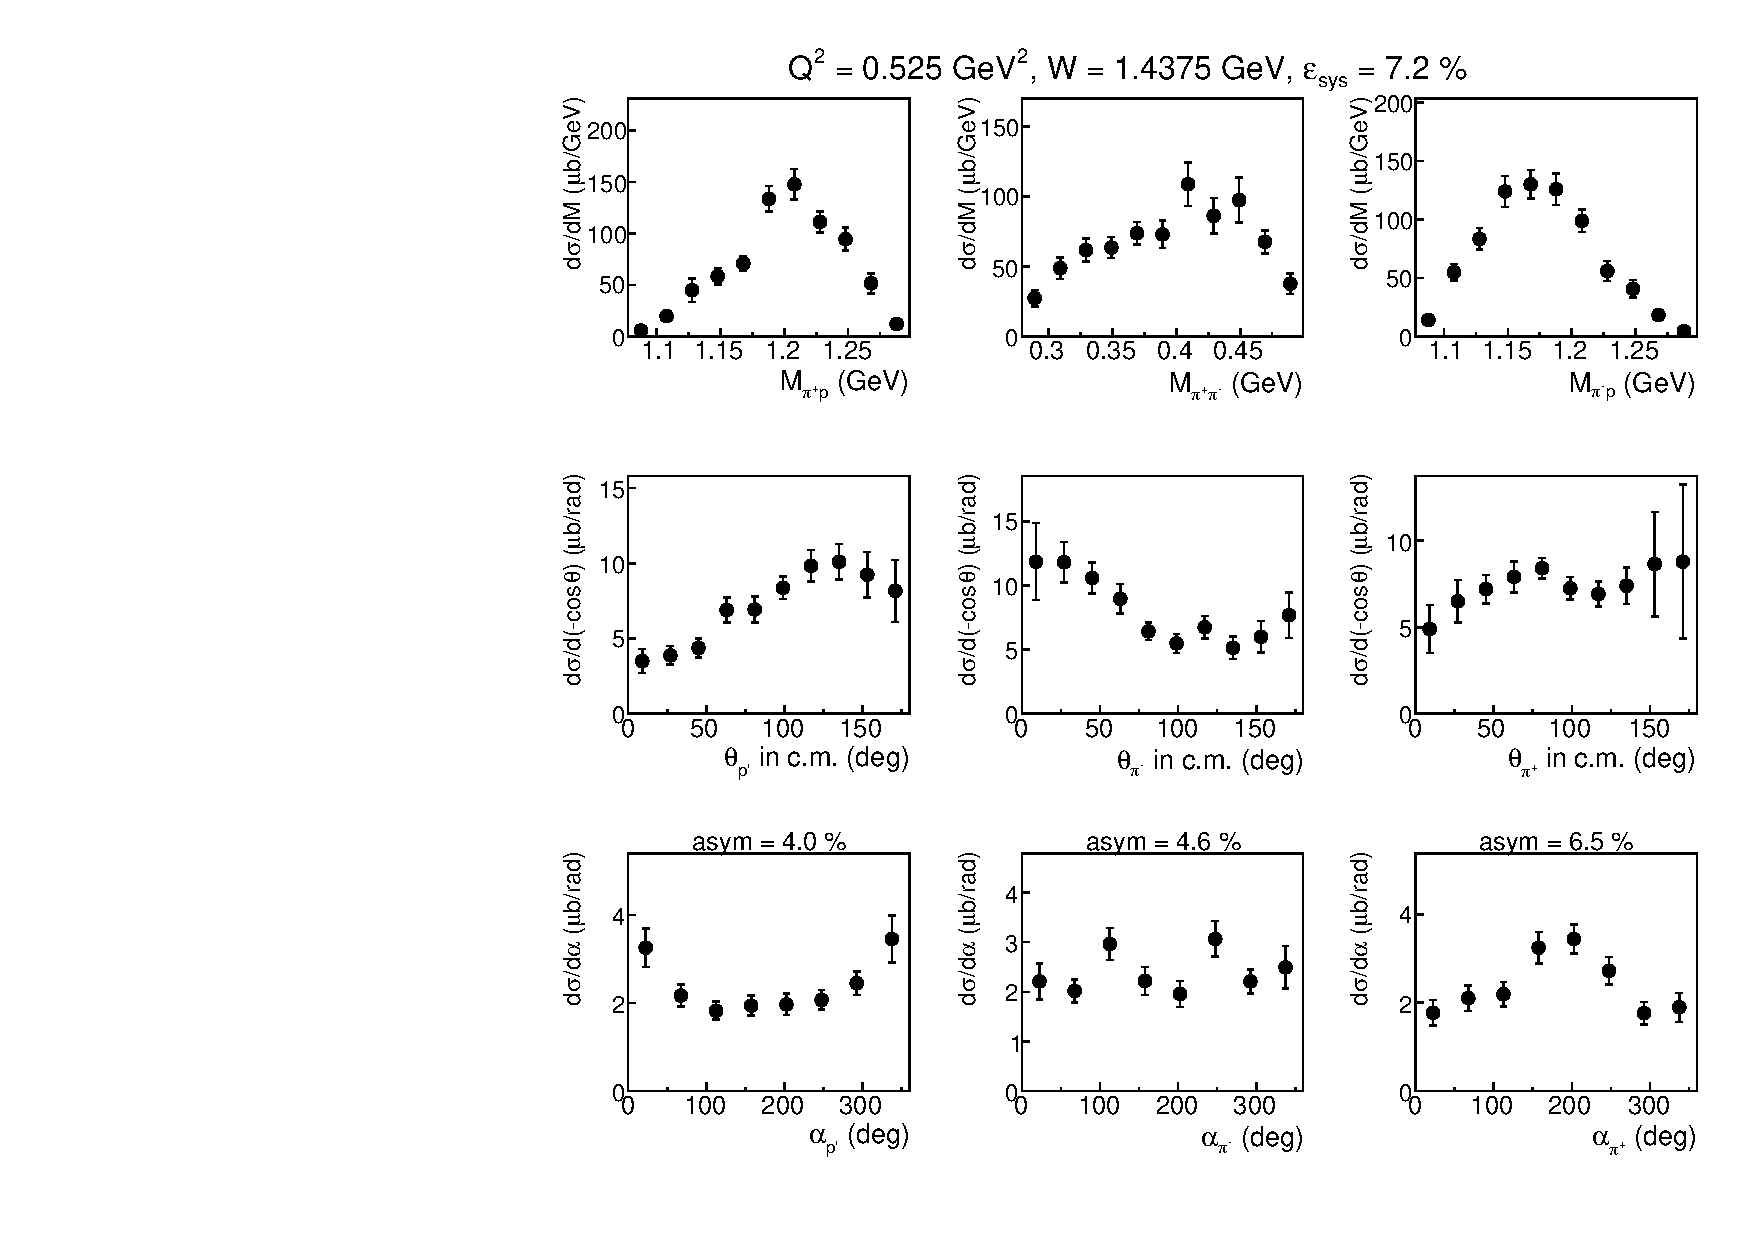
\includegraphics[width=0.495\textwidth]{pictures/appendix/1diff_distr/Q2_525/w_14375.pdf}}
\frame{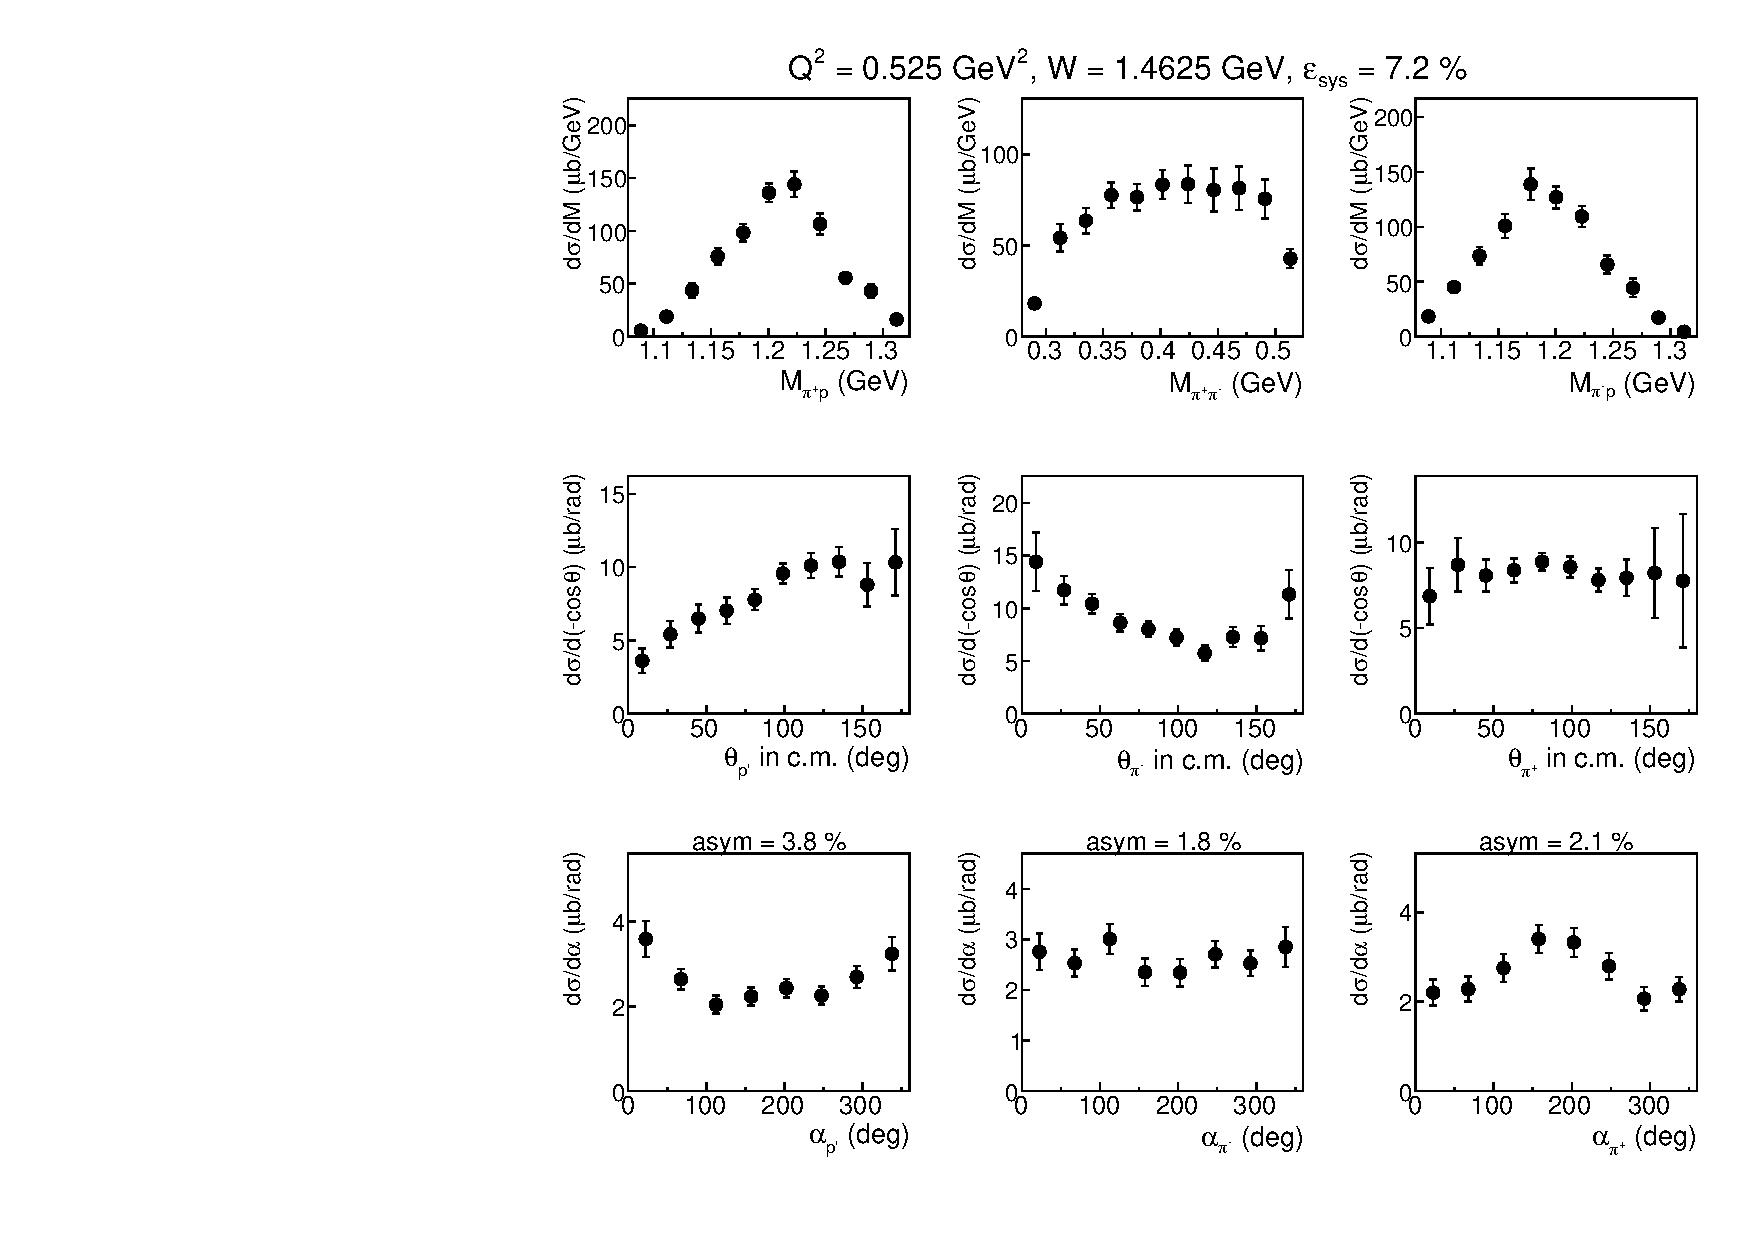
\includegraphics[width=0.495\textwidth]{pictures/appendix/1diff_distr/Q2_525/w_14625.pdf}}
\frame{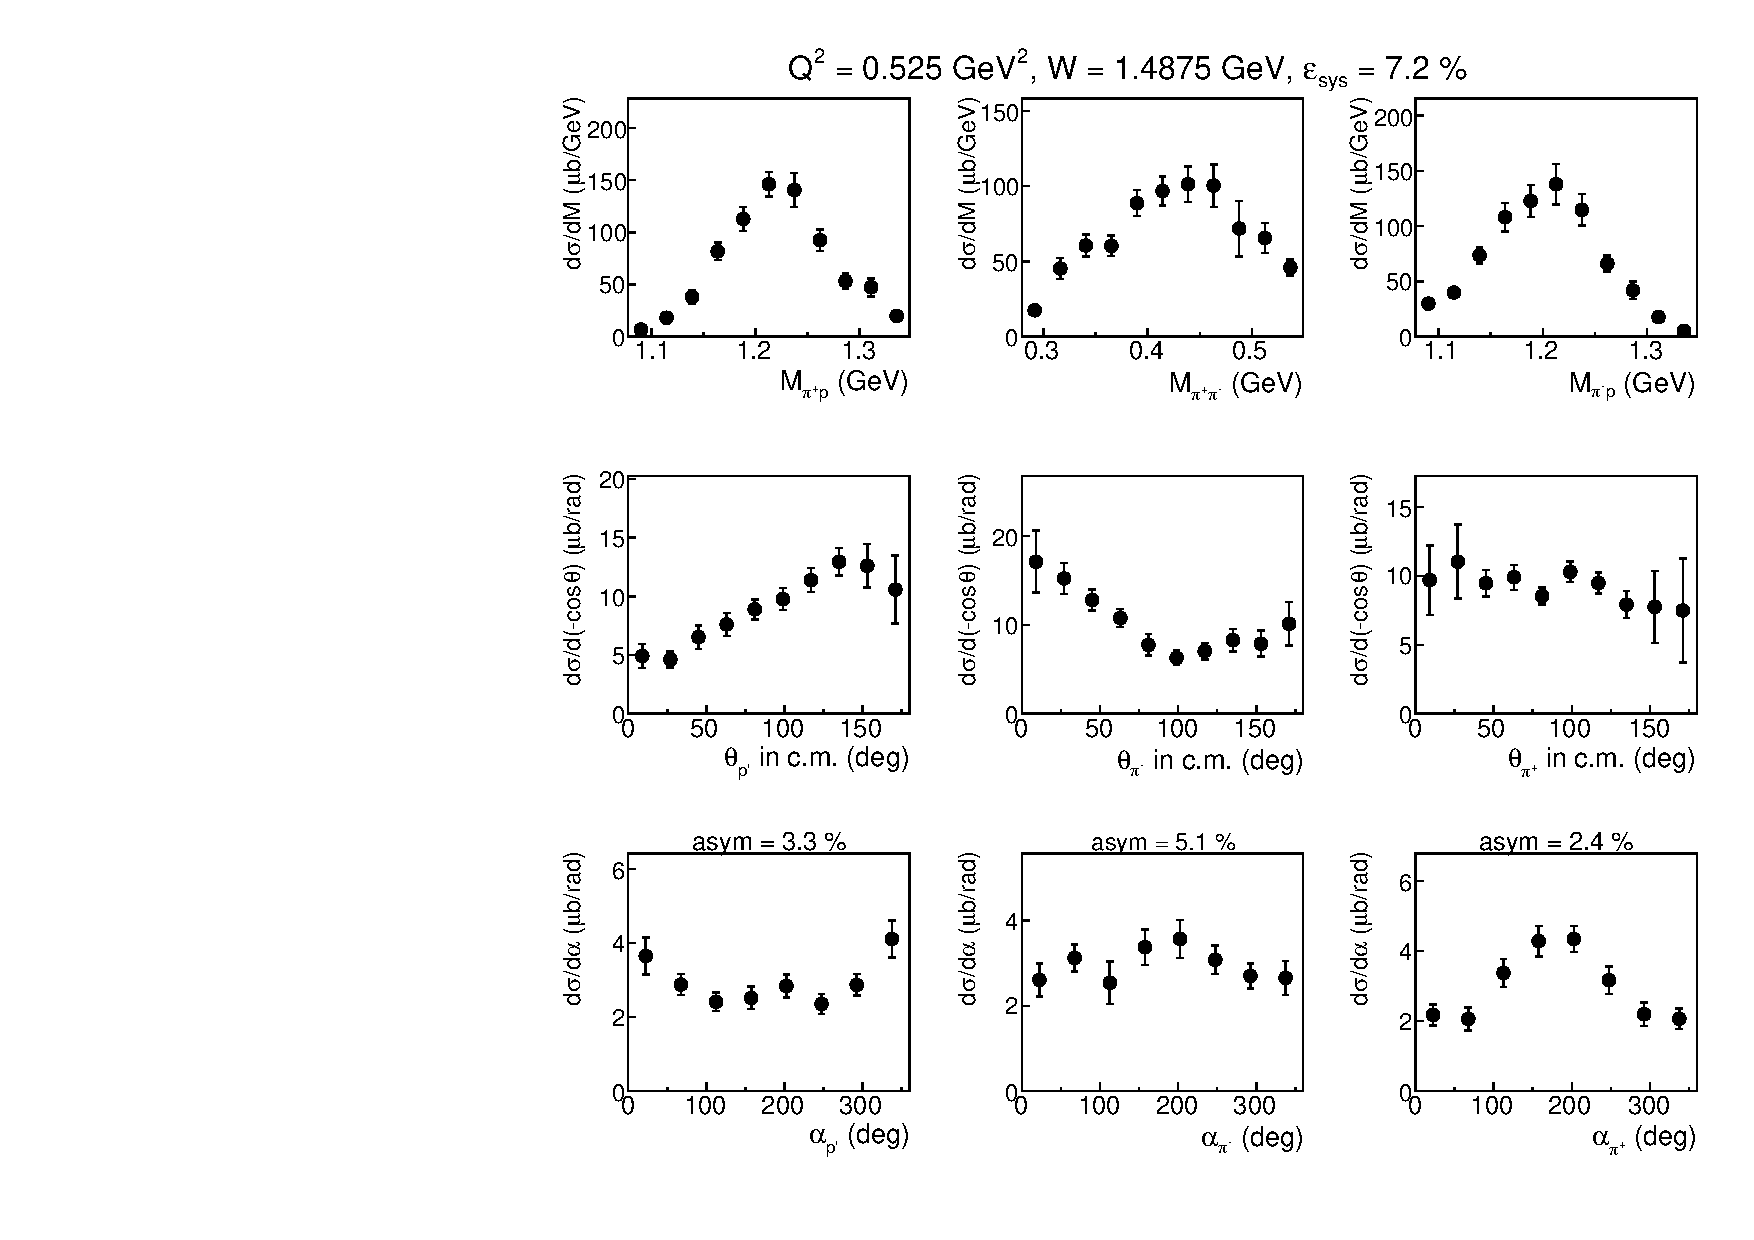
\includegraphics[width=0.495\textwidth]{pictures/appendix/1diff_distr/Q2_525/w_14875.pdf}}
\frame{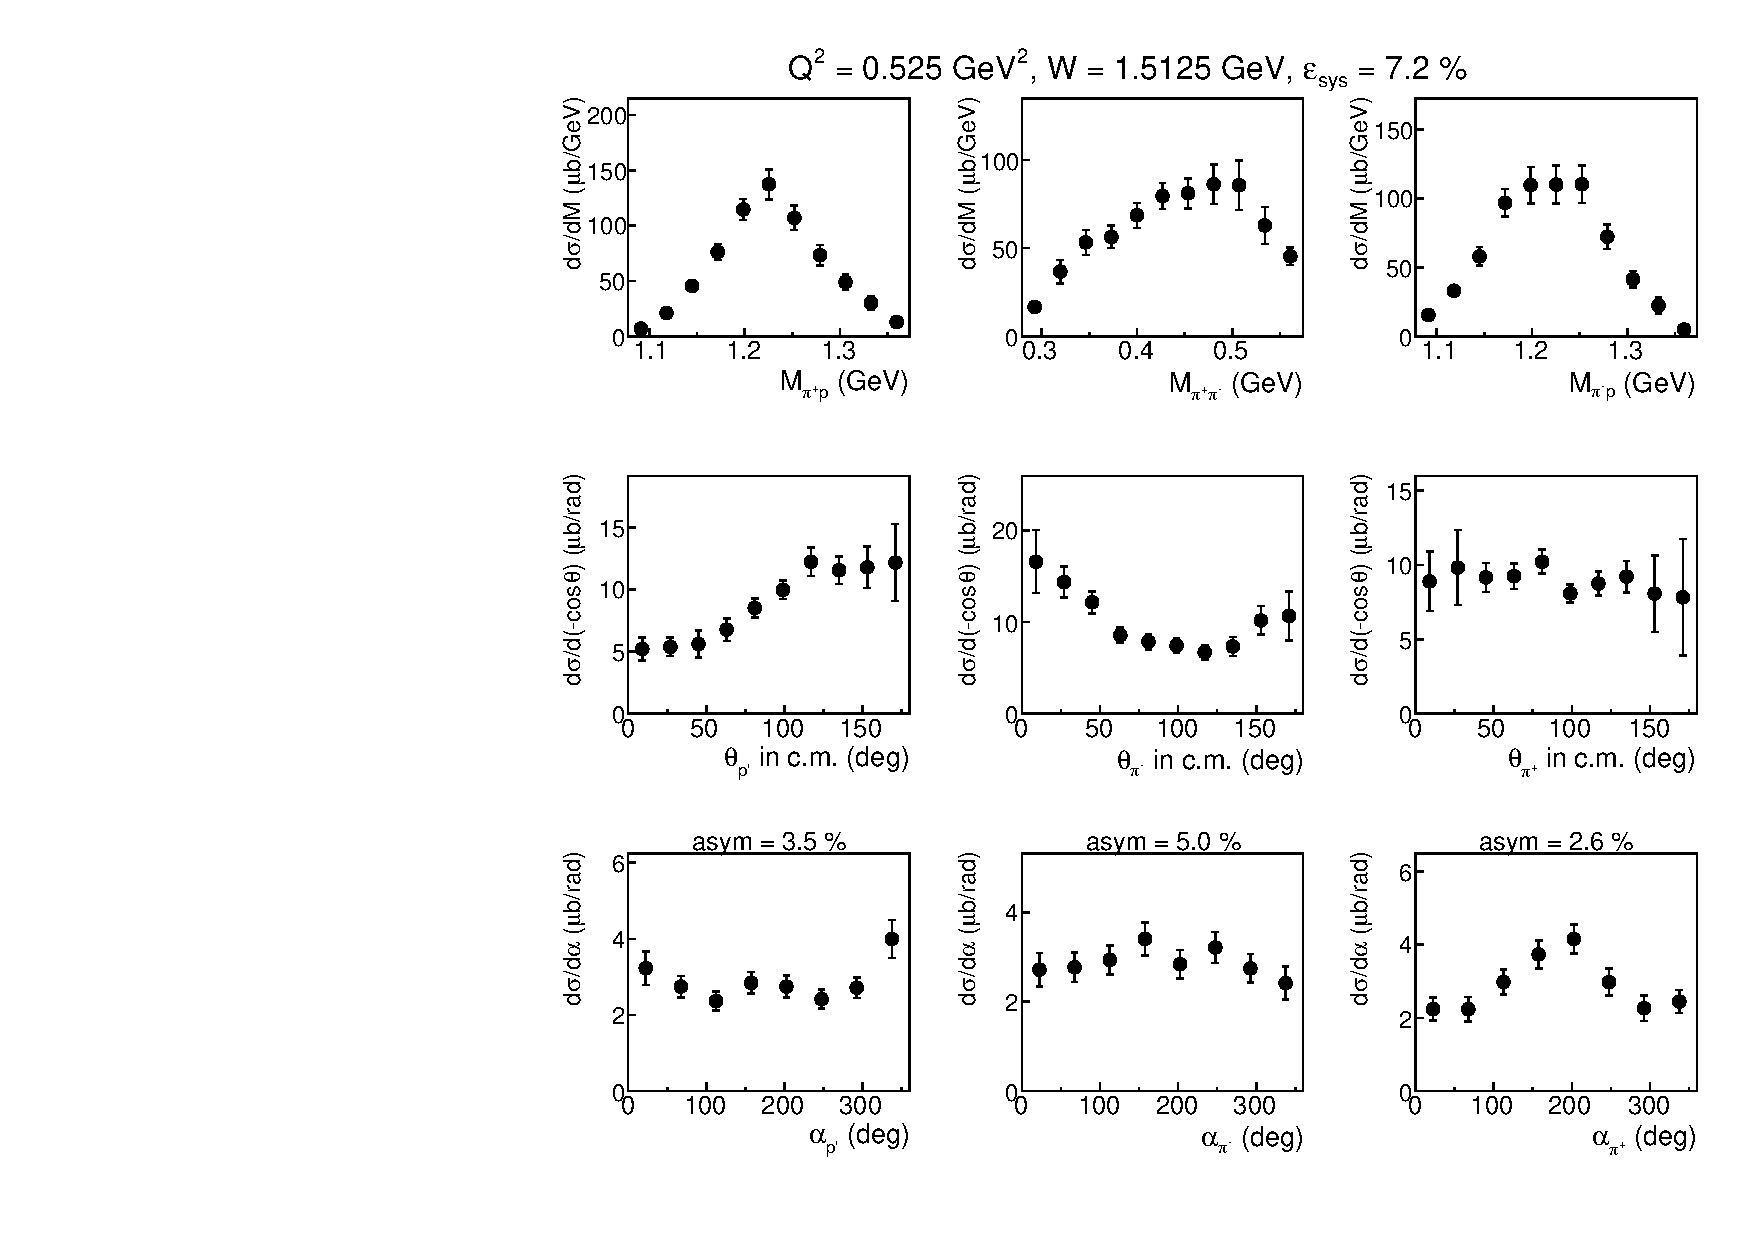
\includegraphics[width=0.495\textwidth]{pictures/appendix/1diff_distr/Q2_525/w_15125.pdf}}
\frame{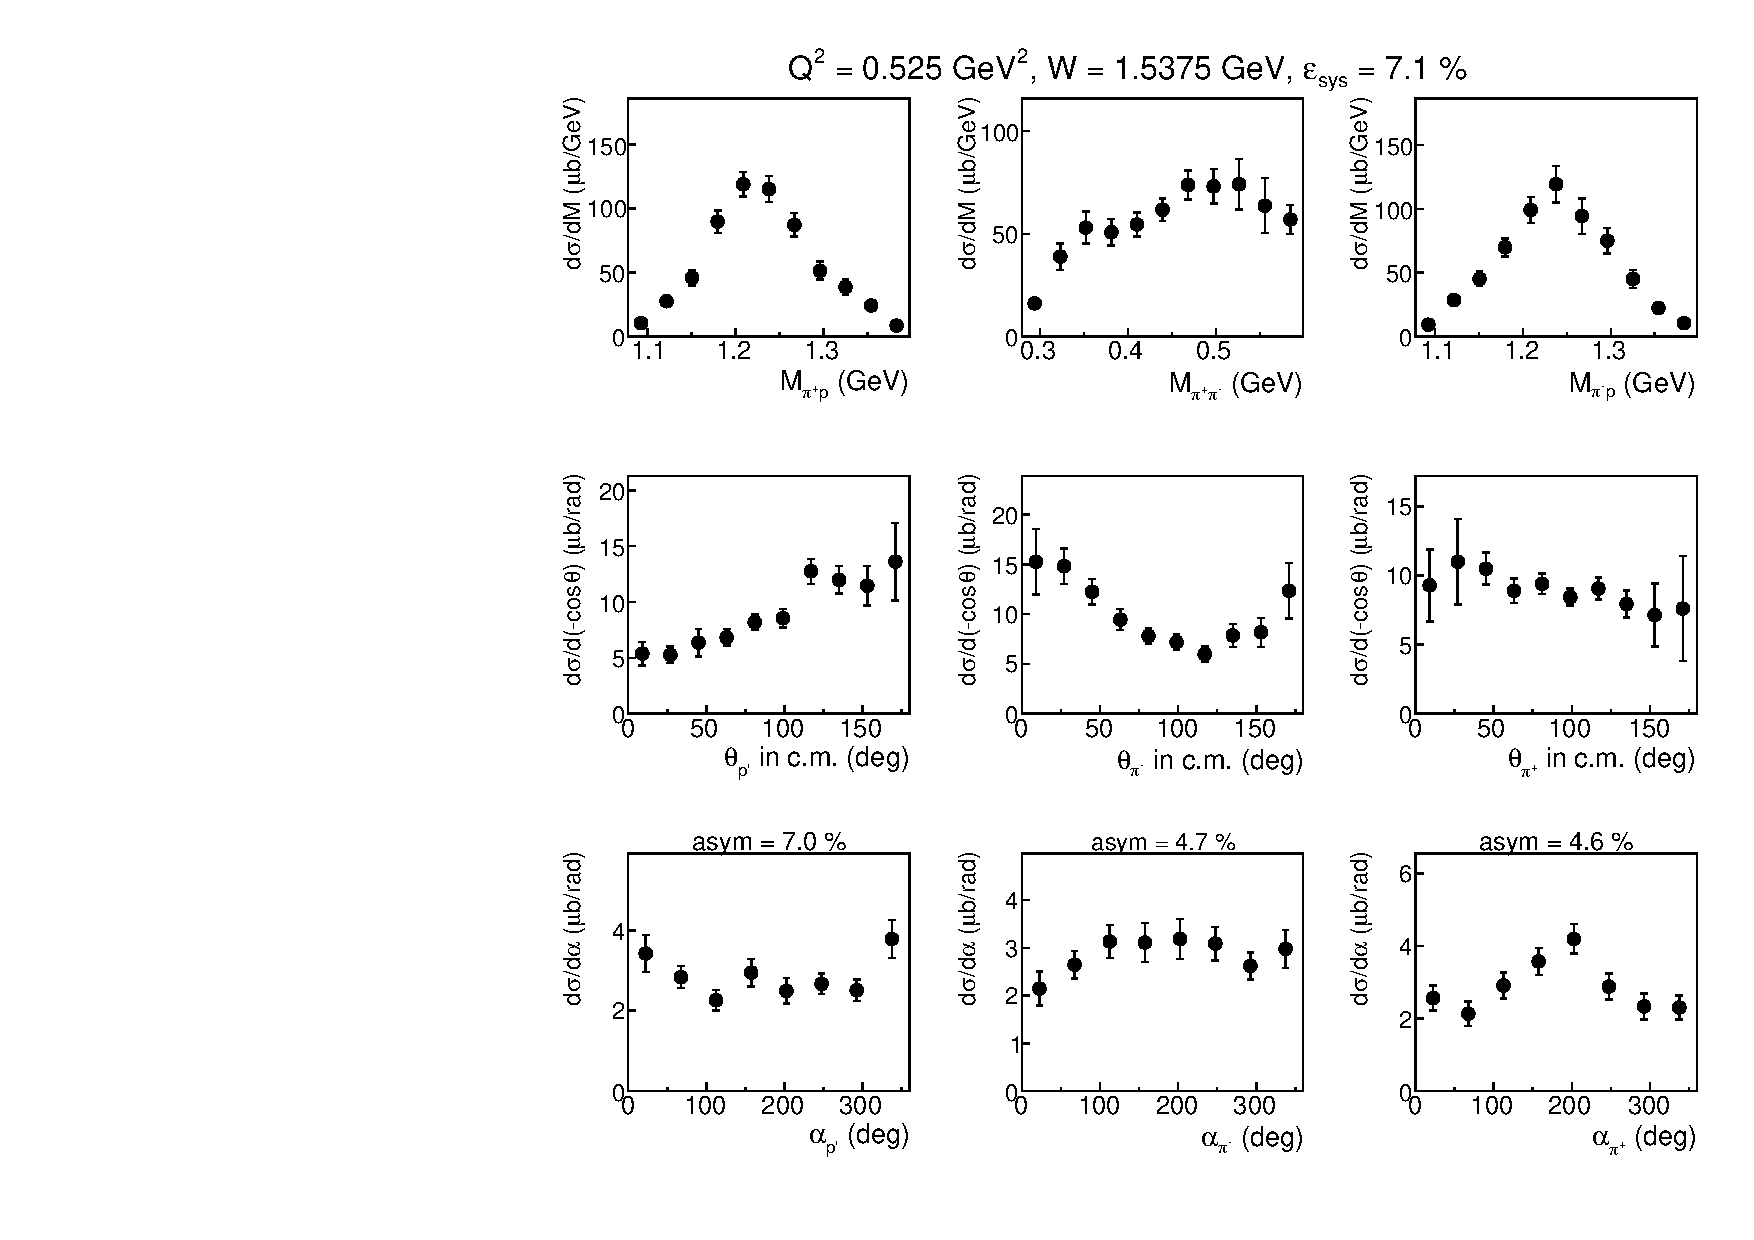
\includegraphics[width=0.495\textwidth]{pictures/appendix/1diff_distr/Q2_525/w_15375.pdf}}
\caption{\small Measured single-differential cross sections.} \label{fig:appx_7}
\end{center}
\end{figure}

\clearpage
\begin{figure}[htp]
\begin{center}
\frame{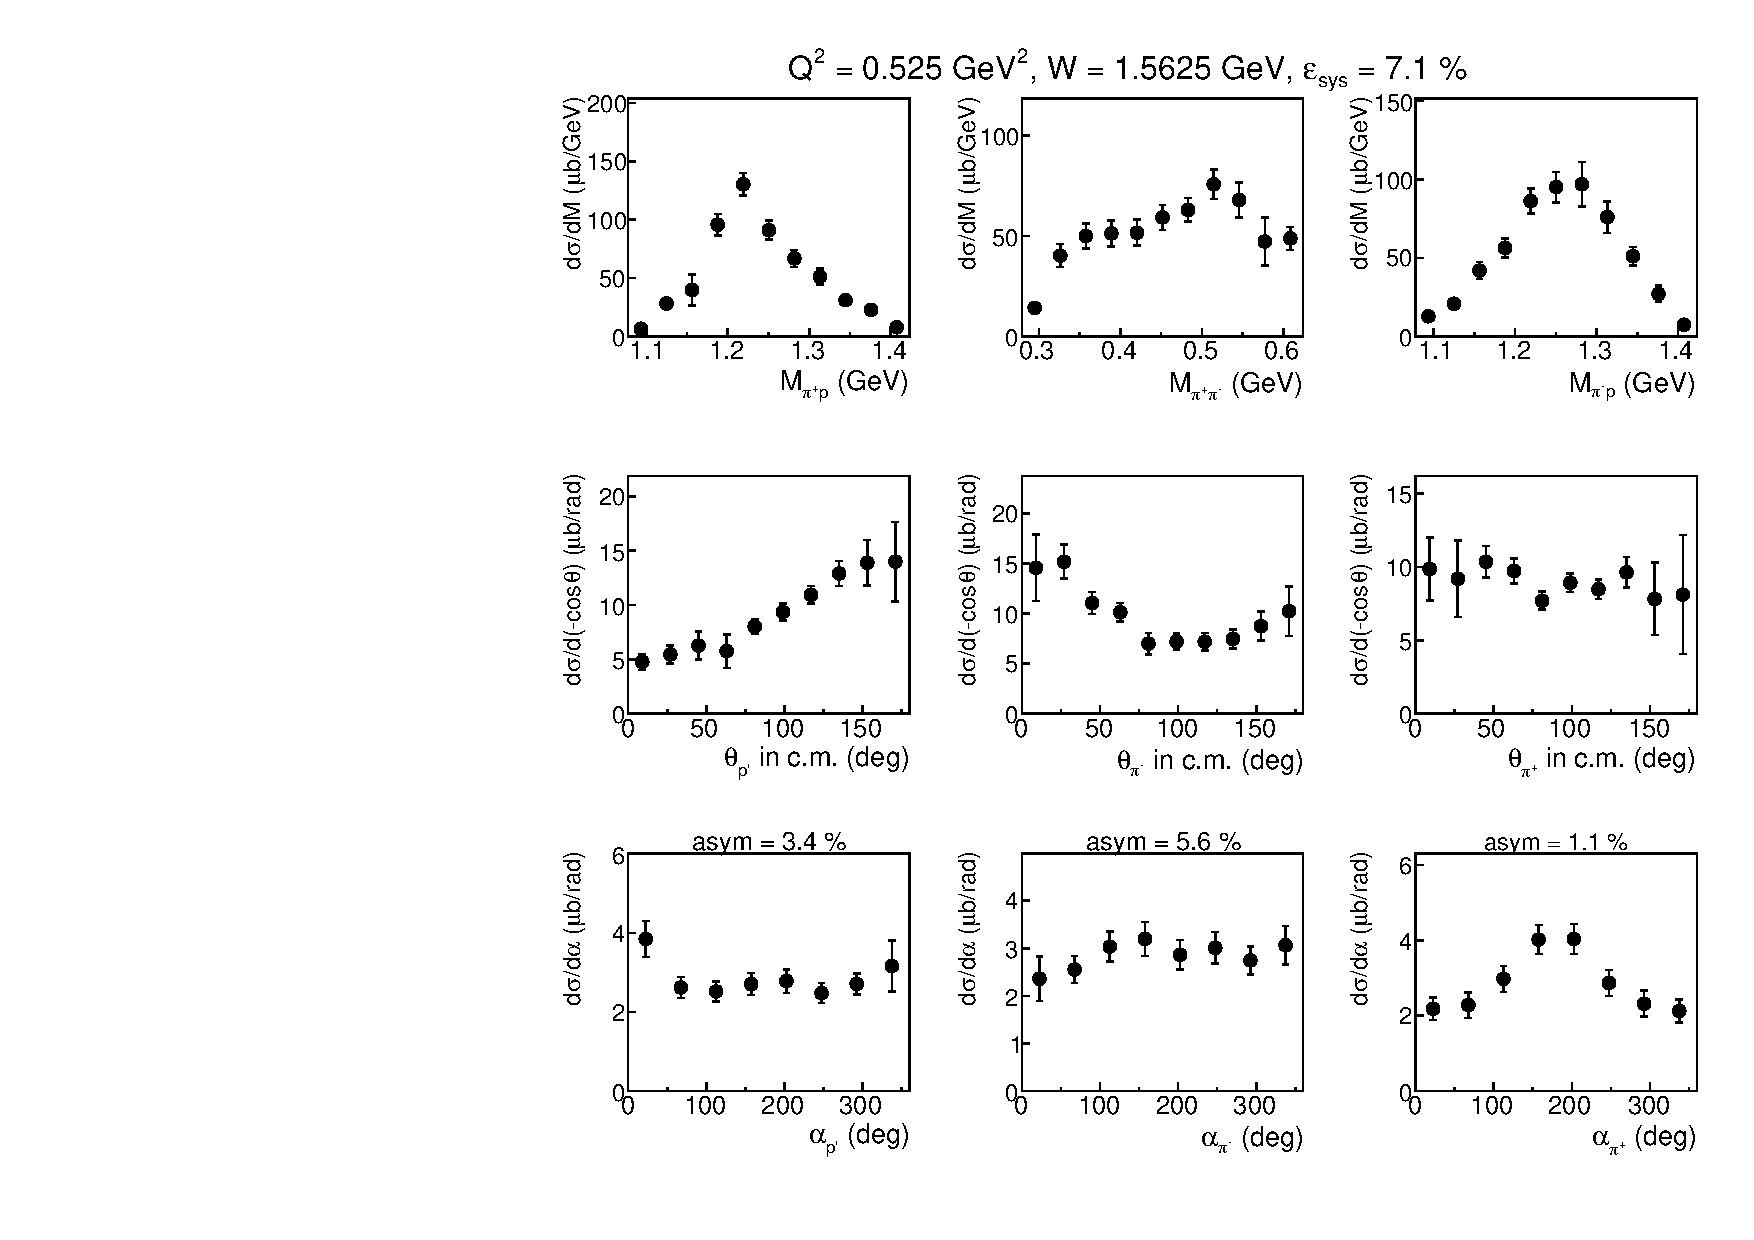
\includegraphics[width=0.495\textwidth]{pictures/appendix/1diff_distr/Q2_525/w_15625.pdf}}
\frame{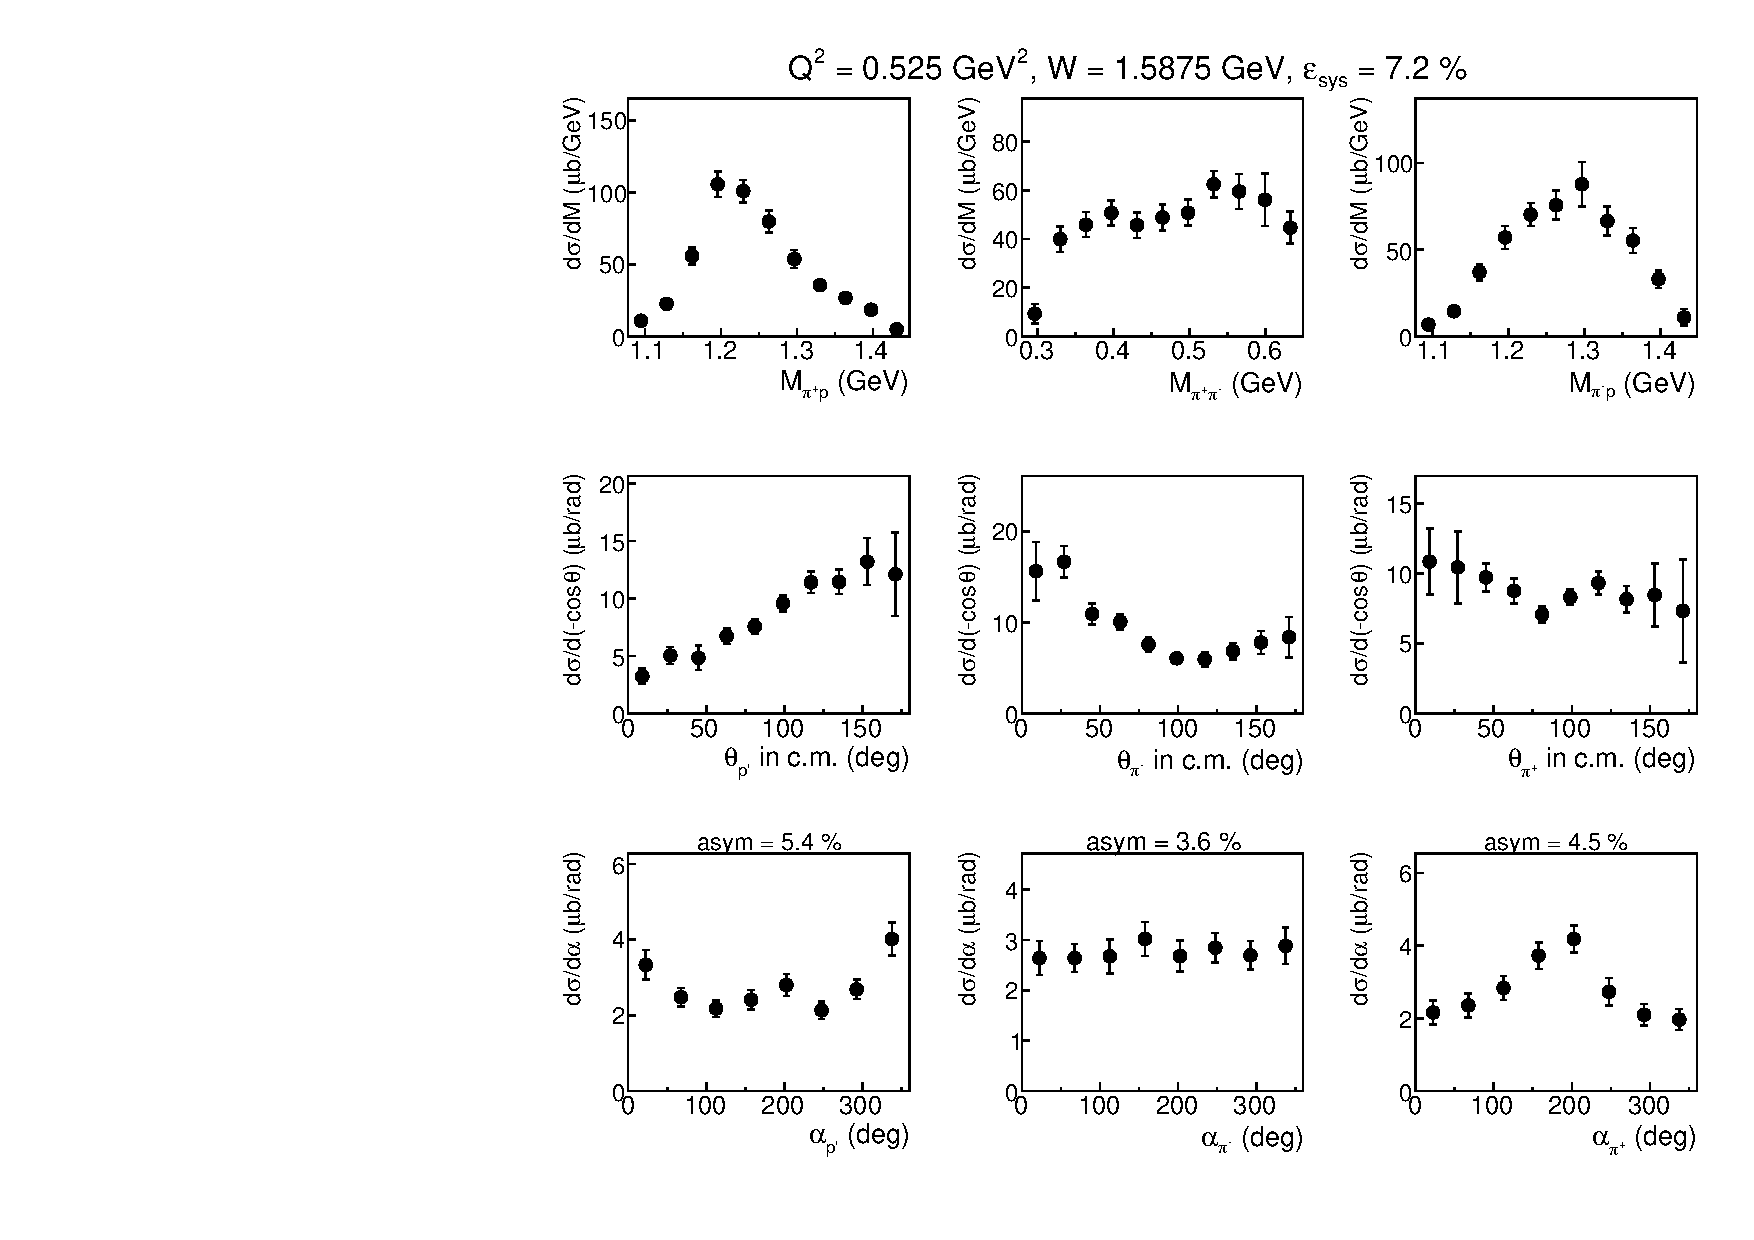
\includegraphics[width=0.495\textwidth]{pictures/appendix/1diff_distr/Q2_525/w_15875.pdf}}
\frame{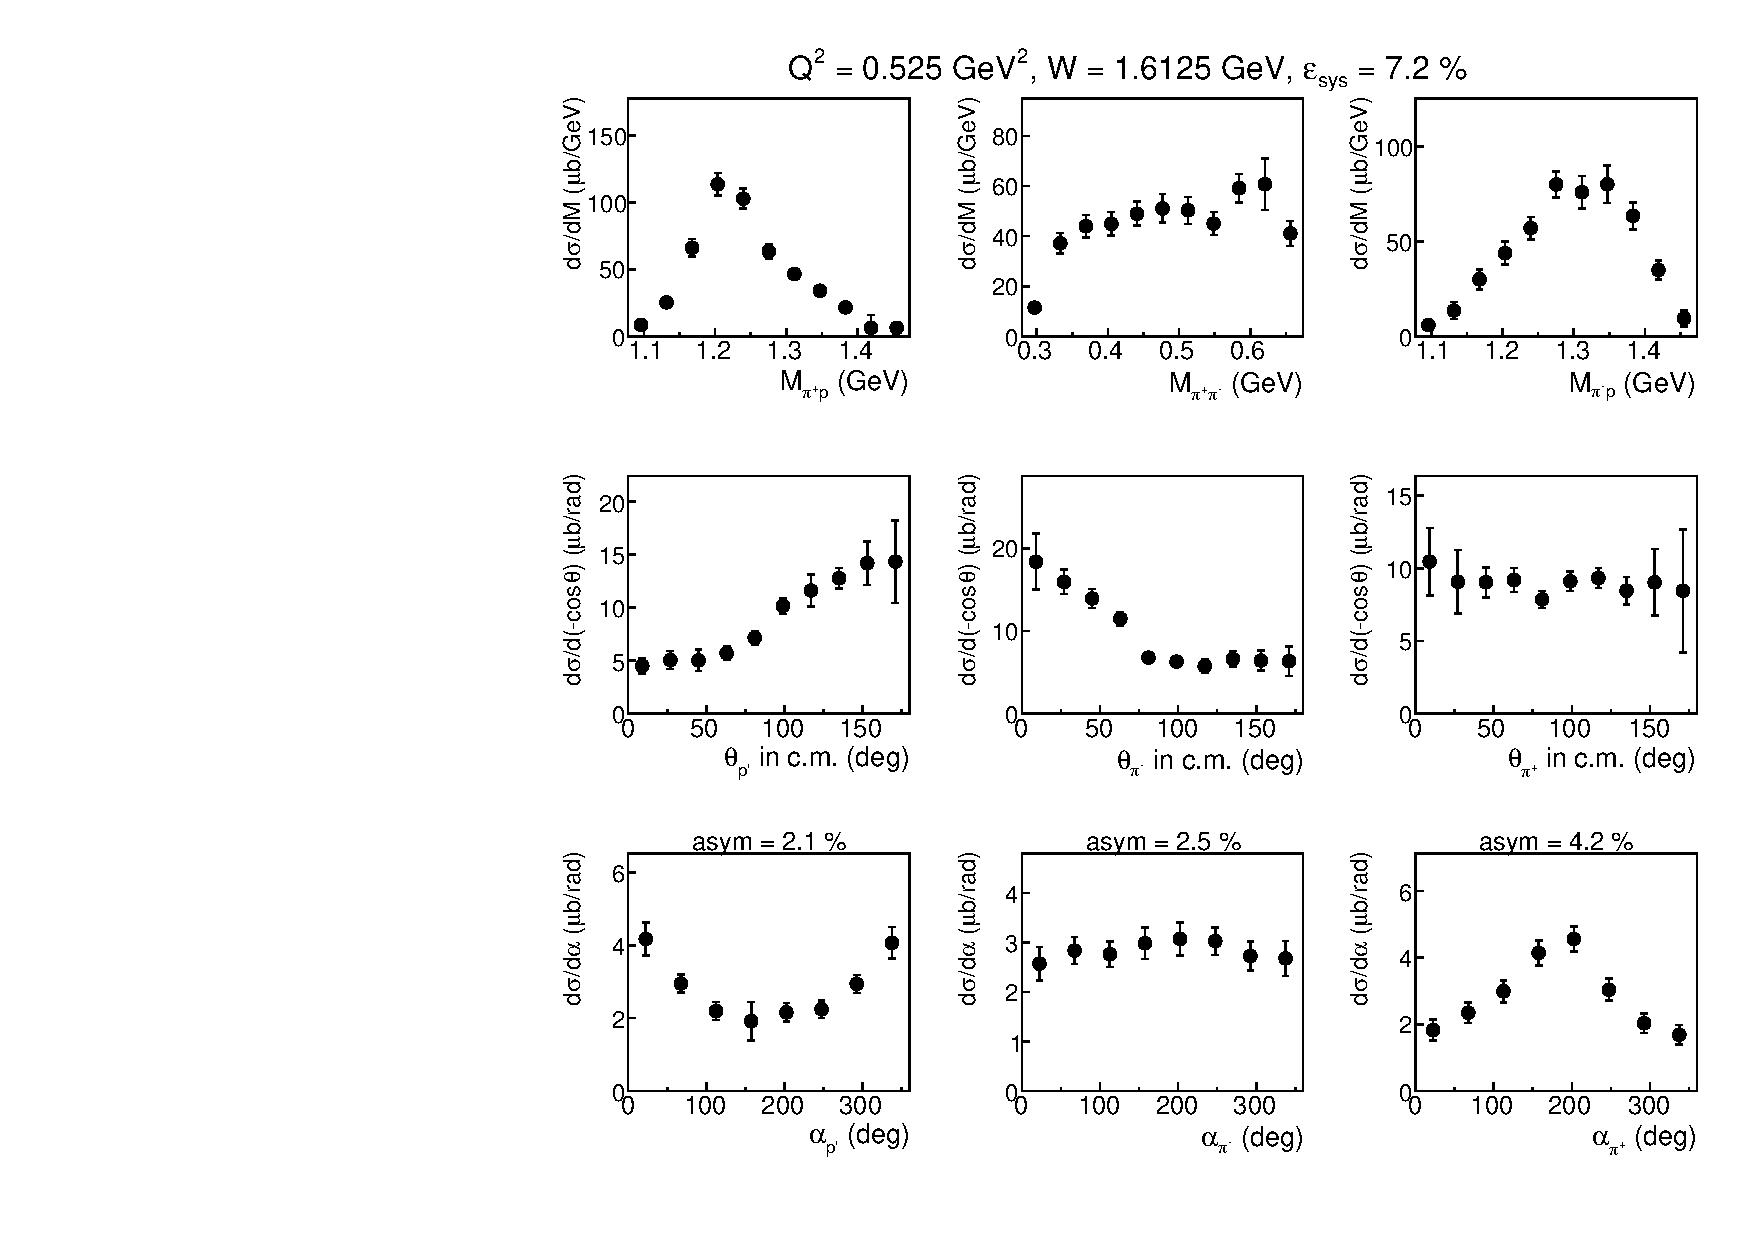
\includegraphics[width=0.495\textwidth]{pictures/appendix/1diff_distr/Q2_525/w_16125.pdf}}
\frame{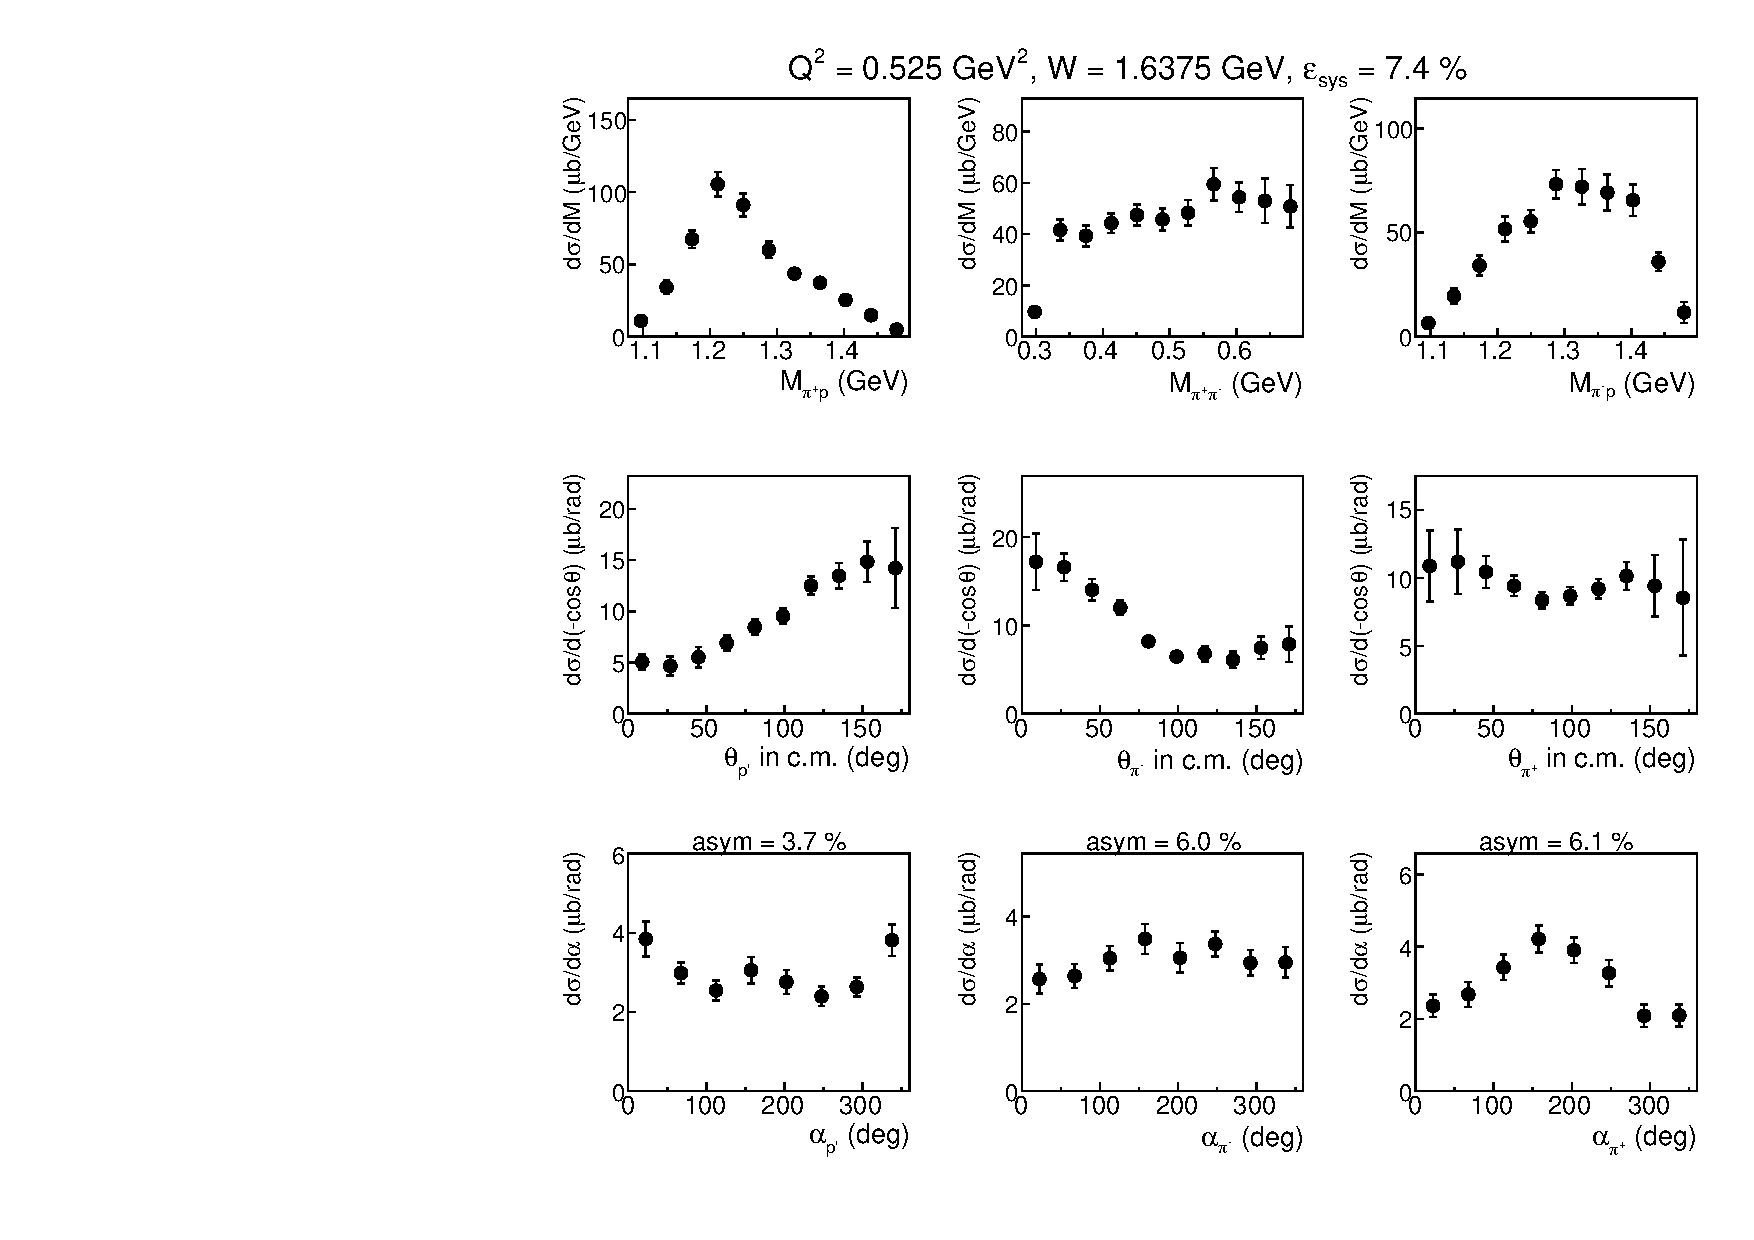
\includegraphics[width=0.495\textwidth]{pictures/appendix/1diff_distr/Q2_525/w_16375.pdf}}
\frame{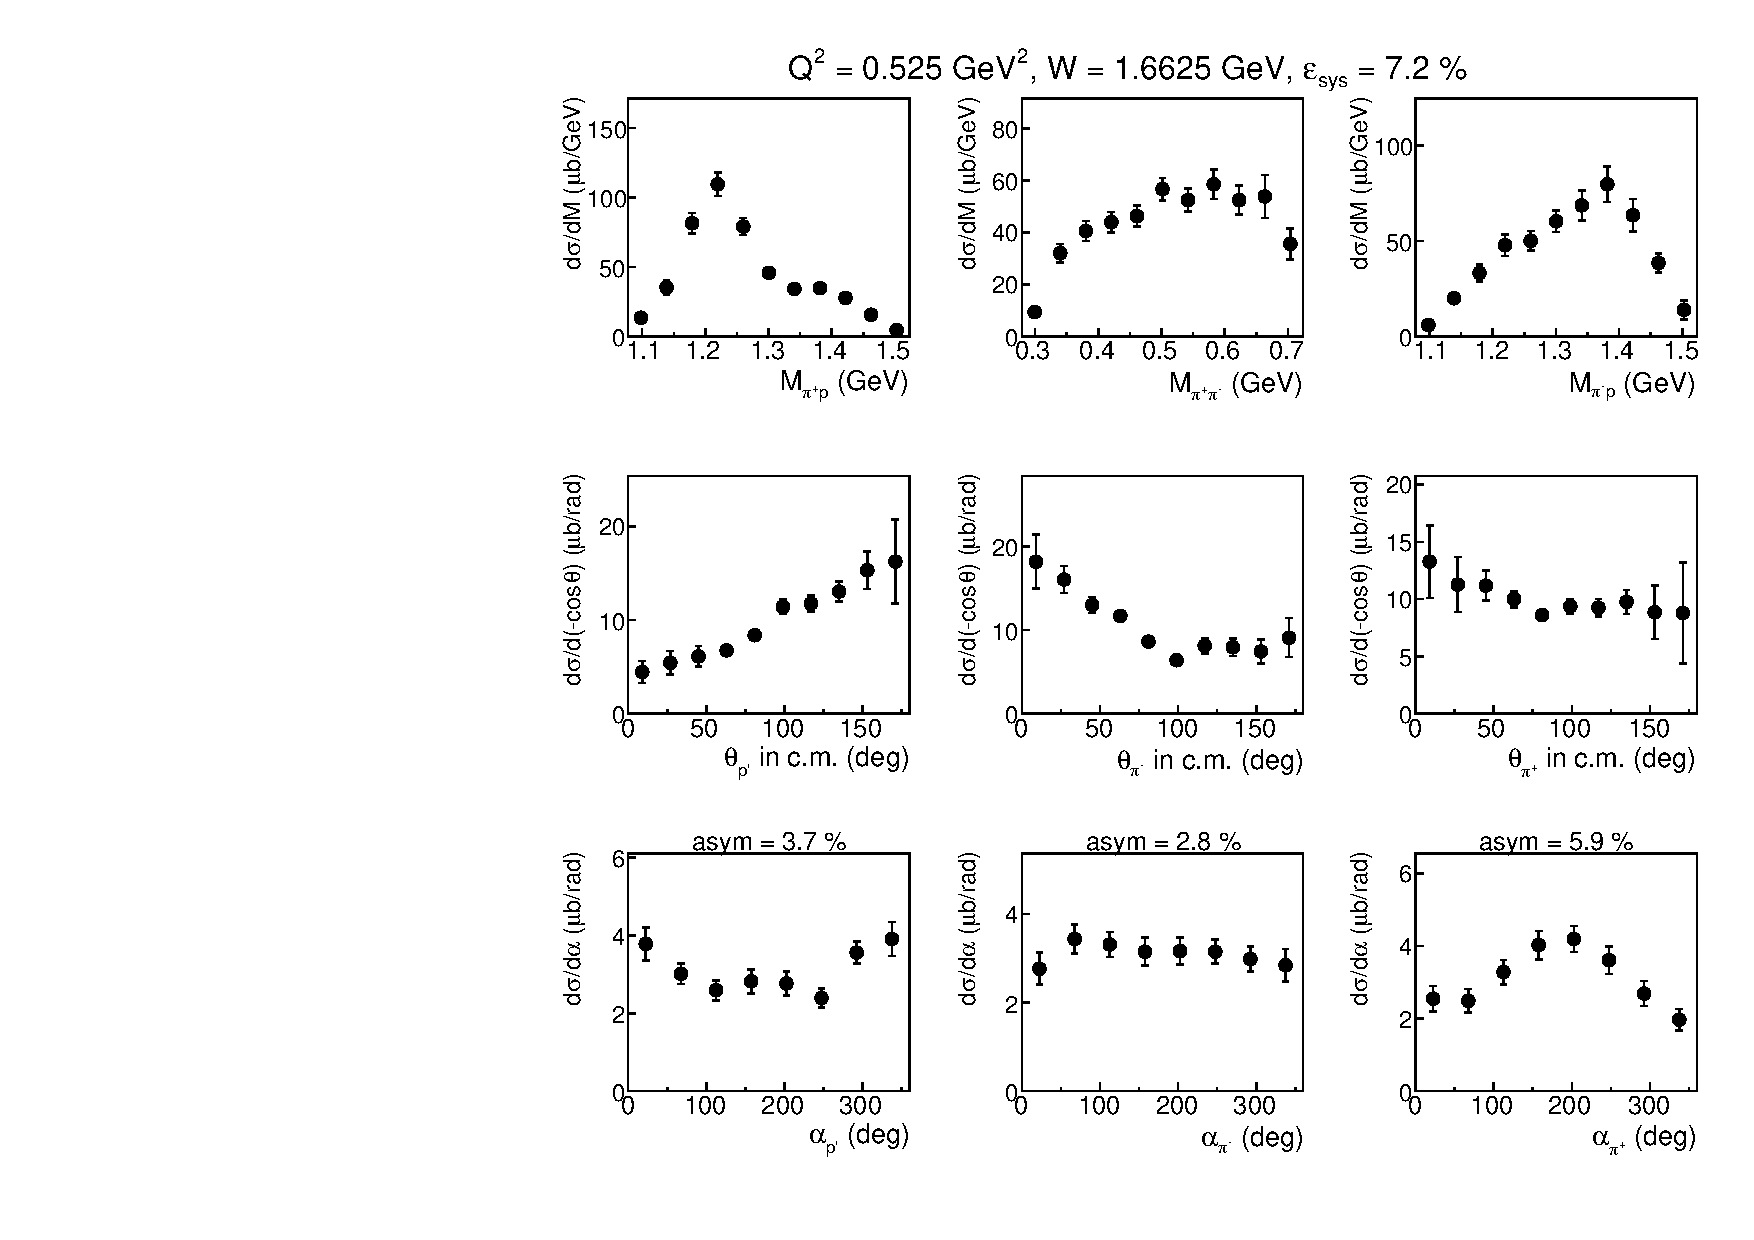
\includegraphics[width=0.495\textwidth]{pictures/appendix/1diff_distr/Q2_525/w_16625.pdf}}
\frame{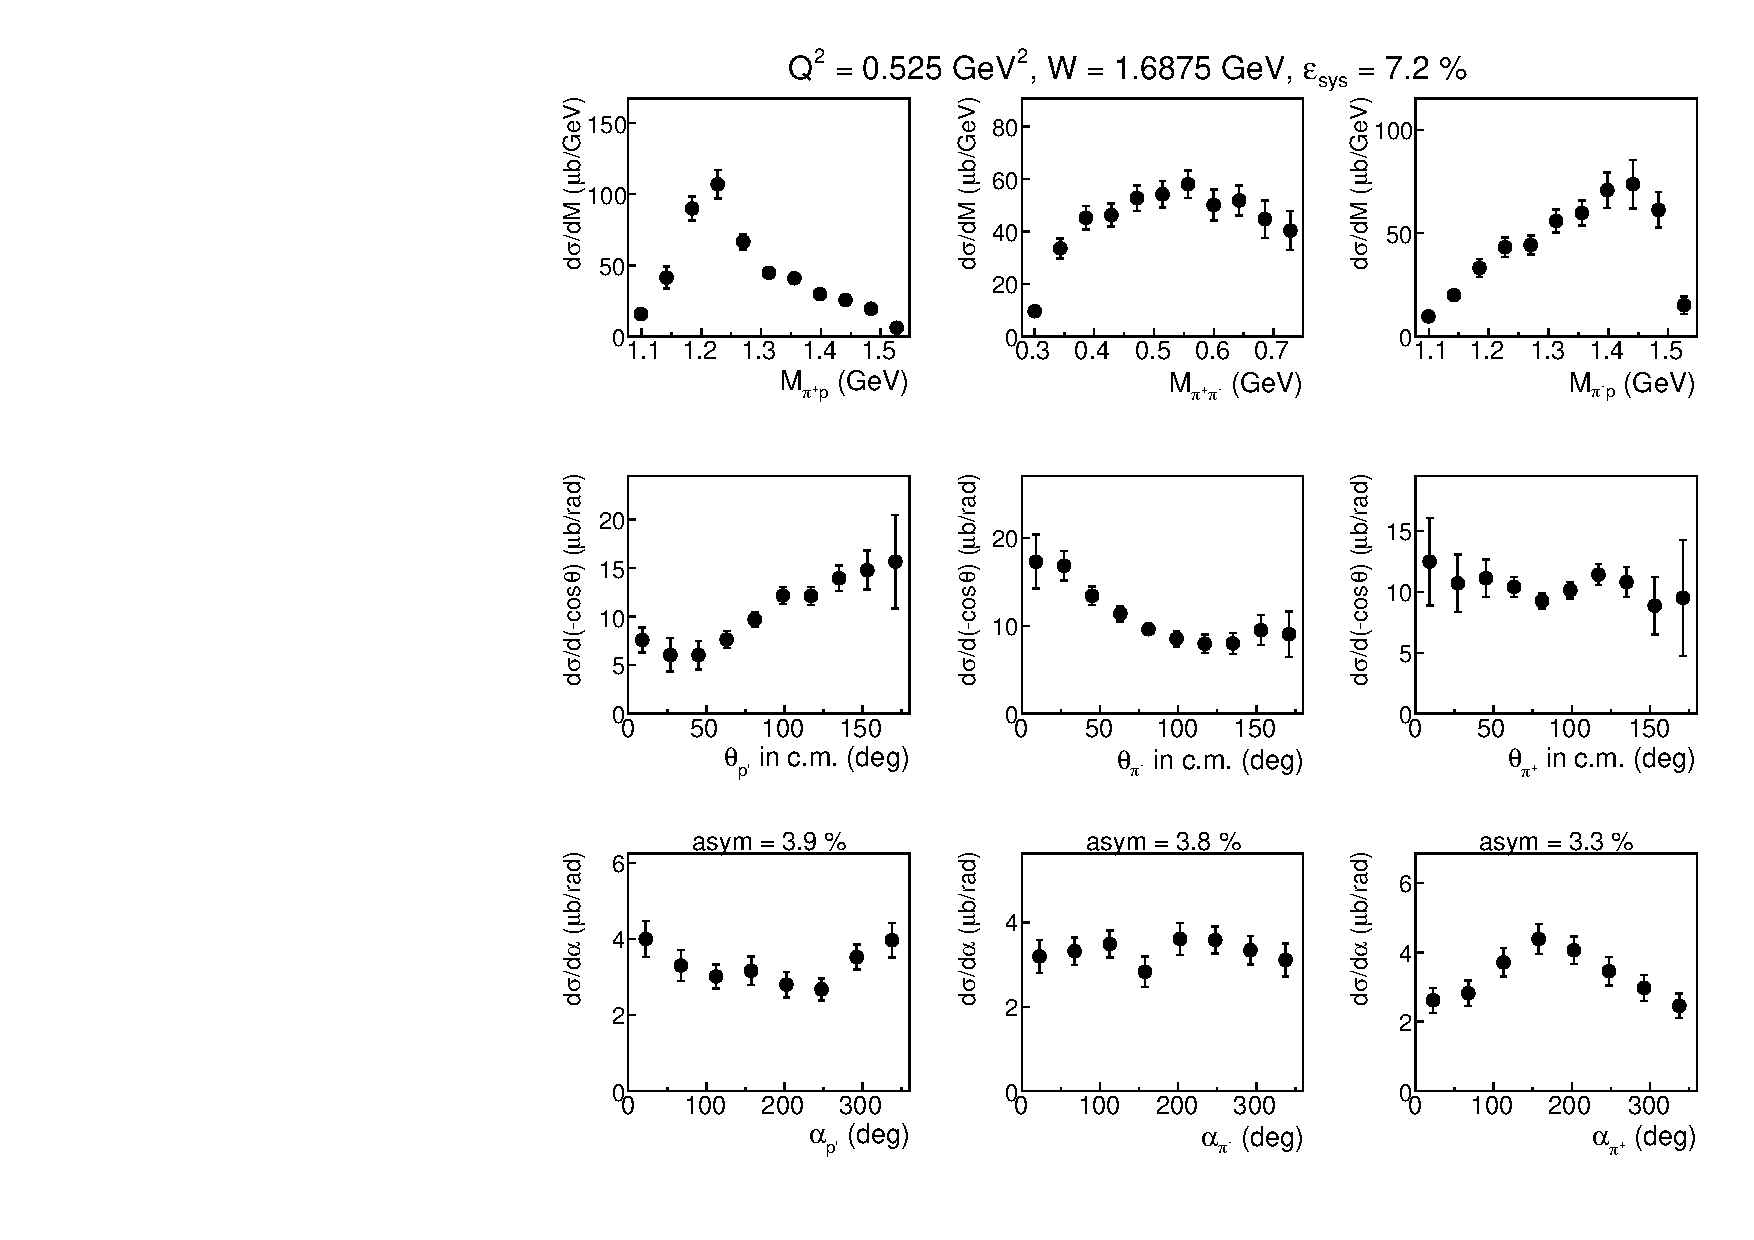
\includegraphics[width=0.495\textwidth]{pictures/appendix/1diff_distr/Q2_525/w_16875.pdf}}
\caption{\small Measured single-differential cross sections.} \label{fig:appx_8}
\end{center}
\end{figure}

\clearpage
\begin{figure}[htp]
\begin{center}
\frame{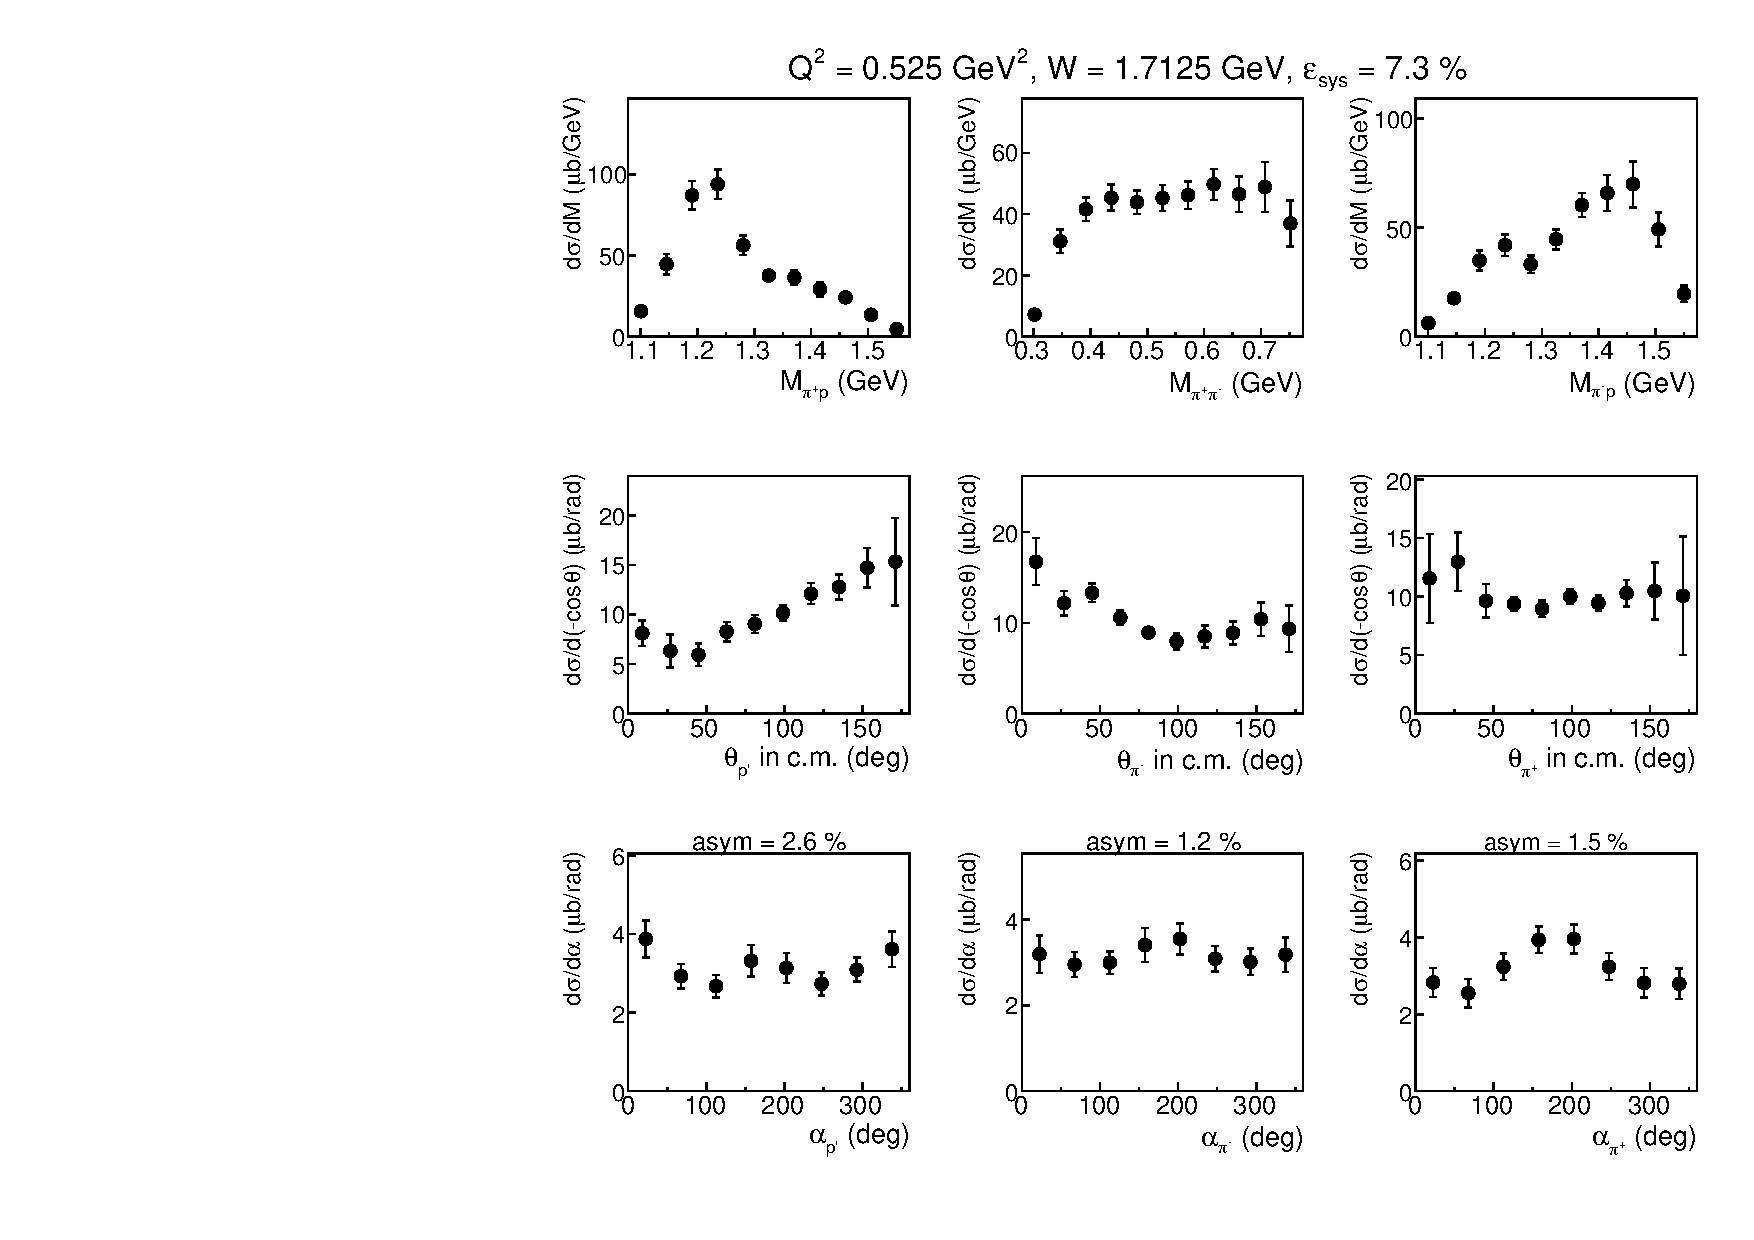
\includegraphics[width=0.495\textwidth]{pictures/appendix/1diff_distr/Q2_525/w_17125.pdf}}
\frame{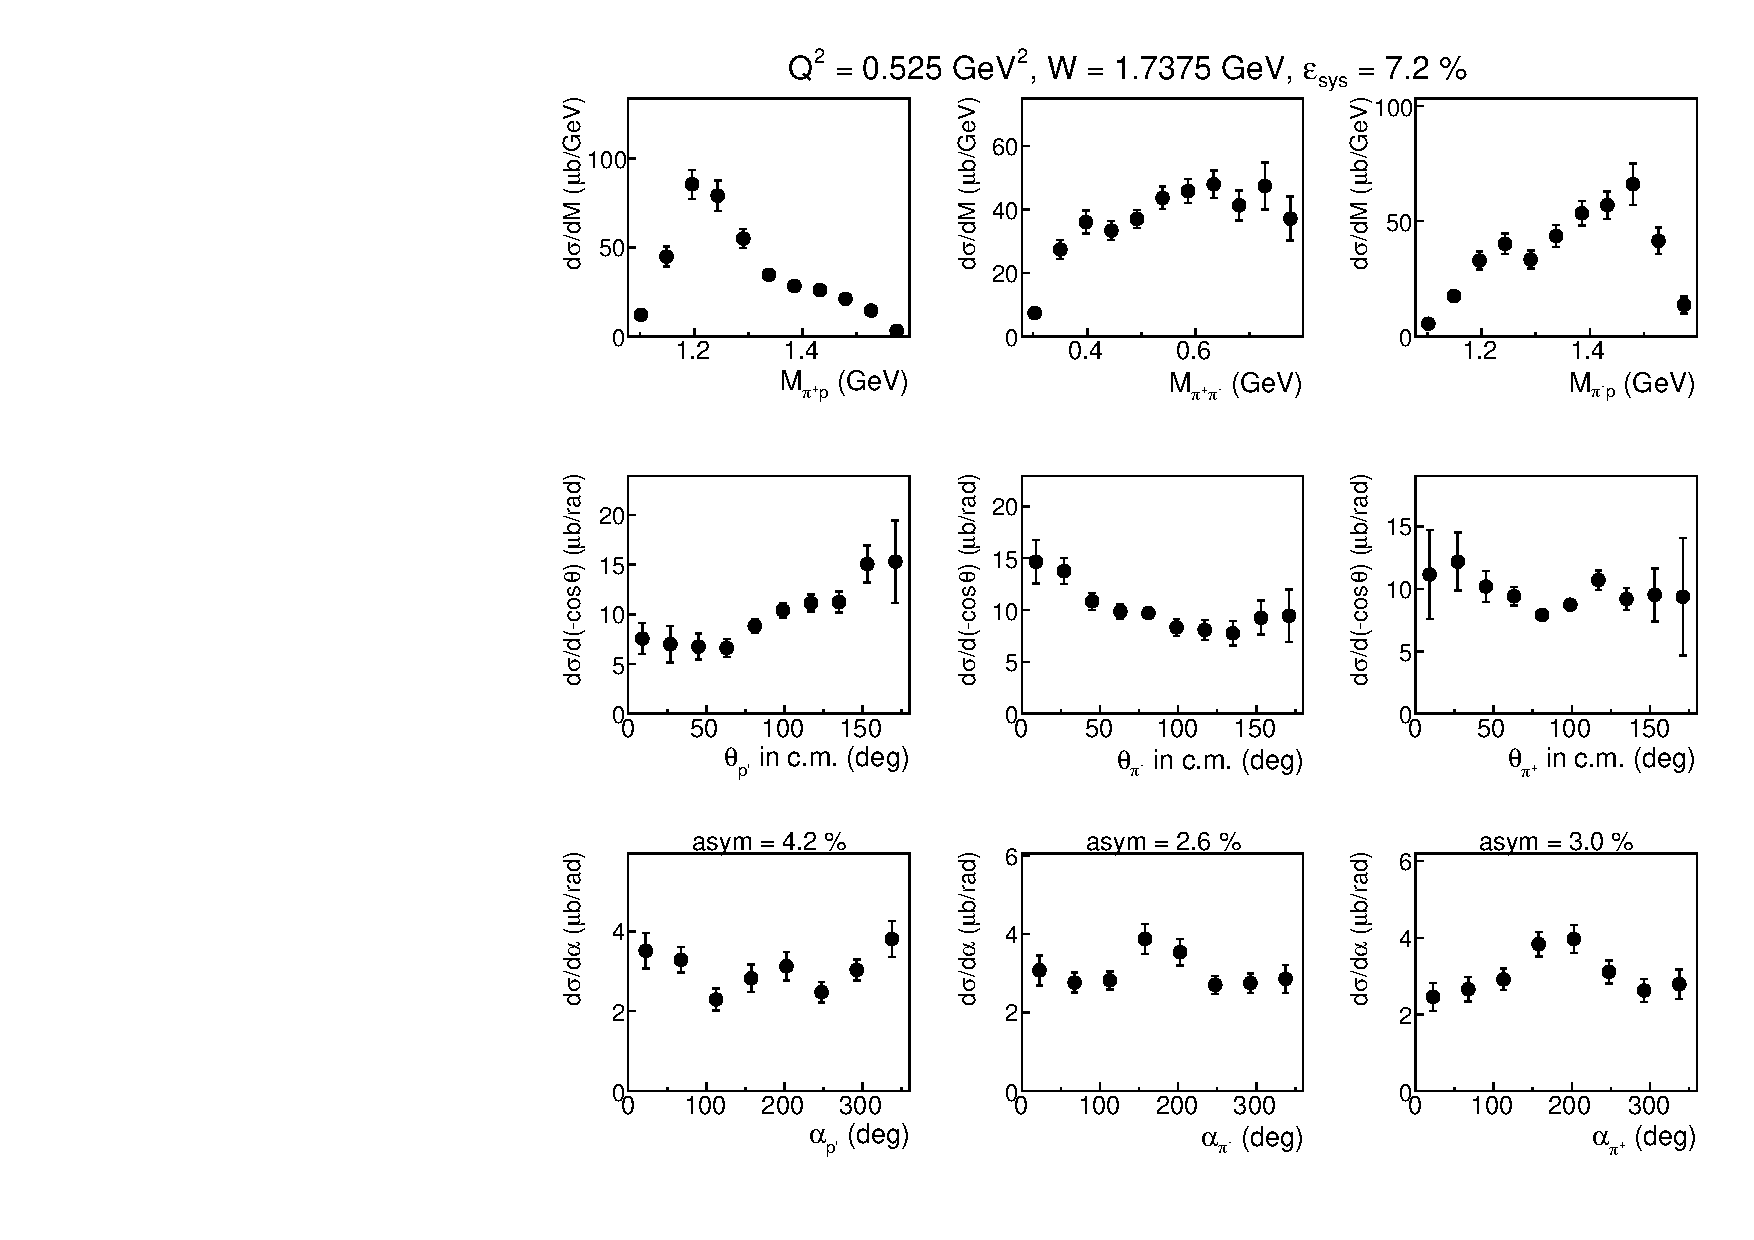
\includegraphics[width=0.495\textwidth]{pictures/appendix/1diff_distr/Q2_525/w_17375.pdf}}
\frame{\includegraphics[width=0.495\textwidth]{pictures/appendix/1diff_distr/Q2_525/w_17625.pdf}}
\frame{\includegraphics[width=0.495\textwidth]{pictures/appendix/1diff_distr/Q2_525/w_17875.pdf}}
\frame{\includegraphics[width=0.495\textwidth]{pictures/appendix/1diff_distr/Q2_575/w_13125.pdf}}
\frame{\includegraphics[width=0.495\textwidth]{pictures/appendix/1diff_distr/Q2_575/w_13375.pdf}}
\caption{\small Measured single-differential cross sections.} \label{fig:appx_9}
\end{center}
\end{figure}

\clearpage
\begin{figure}[htp]
\begin{center}
\frame{\includegraphics[width=0.495\textwidth]{pictures/appendix/1diff_distr/Q2_575/w_13625.pdf}}
\frame{\includegraphics[width=0.495\textwidth]{pictures/appendix/1diff_distr/Q2_575/w_13875.pdf}}
\frame{\includegraphics[width=0.495\textwidth]{pictures/appendix/1diff_distr/Q2_575/w_14125.pdf}}
\frame{\includegraphics[width=0.495\textwidth]{pictures/appendix/1diff_distr/Q2_575/w_14375.pdf}}
\frame{\includegraphics[width=0.495\textwidth]{pictures/appendix/1diff_distr/Q2_575/w_14625.pdf}}
\frame{\includegraphics[width=0.495\textwidth]{pictures/appendix/1diff_distr/Q2_575/w_14875.pdf}}
\caption{\small Measured single-differential cross sections.} \label{fig:appx_10}
\end{center}
\end{figure}

\clearpage
\begin{figure}[htp]
\begin{center}
\frame{\includegraphics[width=0.495\textwidth]{pictures/appendix/1diff_distr/Q2_575/w_15125.pdf}}
\frame{\includegraphics[width=0.495\textwidth]{pictures/appendix/1diff_distr/Q2_575/w_15375.pdf}}
\frame{\includegraphics[width=0.495\textwidth]{pictures/appendix/1diff_distr/Q2_575/w_15625.pdf}}
\frame{\includegraphics[width=0.495\textwidth]{pictures/appendix/1diff_distr/Q2_575/w_15875.pdf}}
\frame{\includegraphics[width=0.495\textwidth]{pictures/appendix/1diff_distr/Q2_575/w_16125.pdf}}
\frame{\includegraphics[width=0.495\textwidth]{pictures/appendix/1diff_distr/Q2_575/w_16375.pdf}}
\caption{\small Measured single-differential cross sections.} \label{fig:appx_11}
\end{center}
\end{figure}

\clearpage
\begin{figure}[htp]
\begin{center}
\frame{\includegraphics[width=0.495\textwidth]{pictures/appendix/1diff_distr/Q2_575/w_16625.pdf}}
\frame{\includegraphics[width=0.495\textwidth]{pictures/appendix/1diff_distr/Q2_575/w_16875.pdf}}
\frame{\includegraphics[width=0.495\textwidth]{pictures/appendix/1diff_distr/Q2_575/w_17125.pdf}}
\frame{\includegraphics[width=0.495\textwidth]{pictures/appendix/1diff_distr/Q2_575/w_17375.pdf}}
\frame{\includegraphics[width=0.495\textwidth]{pictures/appendix/1diff_distr/Q2_575/w_17625.pdf}}
\frame{\includegraphics[width=0.495\textwidth]{pictures/appendix/1diff_distr/Q2_575/w_17875.pdf}}
\caption{\small Measured single-differential cross sections.} \label{fig:appx_12}
\end{center}
\end{figure}

\clearpage
\begin{figure}[htp]
\begin{center}
\frame{\includegraphics[width=0.495\textwidth]{pictures/appendix/1diff_distr/Q2_625/w_13125.pdf}}
\frame{\includegraphics[width=0.495\textwidth]{pictures/appendix/1diff_distr/Q2_625/w_13375.pdf}}
\frame{\includegraphics[width=0.495\textwidth]{pictures/appendix/1diff_distr/Q2_625/w_13625.pdf}}
\frame{\includegraphics[width=0.495\textwidth]{pictures/appendix/1diff_distr/Q2_625/w_13875.pdf}}
\frame{\includegraphics[width=0.495\textwidth]{pictures/appendix/1diff_distr/Q2_625/w_14125.pdf}}
\frame{\includegraphics[width=0.495\textwidth]{pictures/appendix/1diff_distr/Q2_625/w_14375.pdf}}
\caption{\small Measured single-differential cross sections.} \label{fig:appx_13}
\end{center}
\end{figure}

\clearpage
\begin{figure}[htp]
\begin{center}
\frame{\includegraphics[width=0.495\textwidth]{pictures/appendix/1diff_distr/Q2_625/w_14625.pdf}}
\frame{\includegraphics[width=0.495\textwidth]{pictures/appendix/1diff_distr/Q2_625/w_14875.pdf}}
\frame{\includegraphics[width=0.495\textwidth]{pictures/appendix/1diff_distr/Q2_625/w_15125.pdf}}
\frame{\includegraphics[width=0.495\textwidth]{pictures/appendix/1diff_distr/Q2_625/w_15375.pdf}}
\frame{\includegraphics[width=0.495\textwidth]{pictures/appendix/1diff_distr/Q2_625/w_15625.pdf}}
\frame{\includegraphics[width=0.495\textwidth]{pictures/appendix/1diff_distr/Q2_625/w_15875.pdf}}
\caption{\small Measured single-differential cross sections.} \label{fig:appx_14}
\end{center}
\end{figure}

\clearpage
\begin{figure}[htp]
\begin{center}
\frame{\includegraphics[width=0.495\textwidth]{pictures/appendix/1diff_distr/Q2_625/w_16125.pdf}}
\frame{\includegraphics[width=0.495\textwidth]{pictures/appendix/1diff_distr/Q2_625/w_16375.pdf}}
\frame{\includegraphics[width=0.495\textwidth]{pictures/appendix/1diff_distr/Q2_625/w_16625.pdf}}
\frame{\includegraphics[width=0.495\textwidth]{pictures/appendix/1diff_distr/Q2_625/w_16875.pdf}}
\frame{\includegraphics[width=0.495\textwidth]{pictures/appendix/1diff_distr/Q2_625/w_17125.pdf}}
\frame{\includegraphics[width=0.495\textwidth]{pictures/appendix/1diff_distr/Q2_625/w_17375.pdf}}
\caption{\small Measured single-differential cross sections.} \label{fig:appx_15}
\end{center}
\end{figure}

\clearpage
\begin{figure}[htp]
\begin{center}
\frame{\includegraphics[width=0.495\textwidth]{pictures/appendix/1diff_distr/Q2_625/w_17625.pdf}}
\frame{\includegraphics[width=0.495\textwidth]{pictures/appendix/1diff_distr/Q2_675/w_13125.pdf}}
\frame{\includegraphics[width=0.495\textwidth]{pictures/appendix/1diff_distr/Q2_675/w_13375.pdf}}
\frame{\includegraphics[width=0.495\textwidth]{pictures/appendix/1diff_distr/Q2_675/w_13625.pdf}}
\frame{\includegraphics[width=0.495\textwidth]{pictures/appendix/1diff_distr/Q2_675/w_13875.pdf}}
\frame{\includegraphics[width=0.495\textwidth]{pictures/appendix/1diff_distr/Q2_675/w_14125.pdf}}
\caption{\small Measured single-differential cross sections.} \label{fig:appx_16}
\end{center}
\end{figure}

\clearpage
\begin{figure}[htp]
\begin{center}
\frame{\includegraphics[width=0.495\textwidth]{pictures/appendix/1diff_distr/Q2_675/w_14375.pdf}}
\frame{\includegraphics[width=0.495\textwidth]{pictures/appendix/1diff_distr/Q2_675/w_14625.pdf}}
\frame{\includegraphics[width=0.495\textwidth]{pictures/appendix/1diff_distr/Q2_675/w_14875.pdf}}
\frame{\includegraphics[width=0.495\textwidth]{pictures/appendix/1diff_distr/Q2_675/w_15125.pdf}}
\frame{\includegraphics[width=0.495\textwidth]{pictures/appendix/1diff_distr/Q2_675/w_15375.pdf}}
\frame{\includegraphics[width=0.495\textwidth]{pictures/appendix/1diff_distr/Q2_675/w_15625.pdf}}
\caption{\small Measured single-differential cross sections.} \label{fig:appx_17}
\end{center}
\end{figure}


\clearpage
\begin{figure}[htp]
\begin{center}
\frame{\includegraphics[width=0.495\textwidth]{pictures/appendix/1diff_distr/Q2_675/w_15875.pdf}}
\frame{\includegraphics[width=0.495\textwidth]{pictures/appendix/1diff_distr/Q2_675/w_16125.pdf}}
\frame{\includegraphics[width=0.495\textwidth]{pictures/appendix/1diff_distr/Q2_675/w_16375.pdf}}
\frame{\includegraphics[width=0.495\textwidth]{pictures/appendix/1diff_distr/Q2_675/w_16625.pdf}}
\frame{\includegraphics[width=0.495\textwidth]{pictures/appendix/1diff_distr/Q2_675/w_16875.pdf}}
\frame{\includegraphics[width=0.495\textwidth]{pictures/appendix/1diff_distr/Q2_675/w_17125.pdf}}
\caption{\small Measured single-differential cross sections.} \label{fig:appx_18}
\end{center}
\end{figure}

\clearpage
\begin{figure}[htp]
\begin{center}
\frame{\includegraphics[width=0.495\textwidth]{pictures/appendix/1diff_distr/Q2_675/w_17375.pdf}}
\frame{\includegraphics[width=0.495\textwidth]{pictures/appendix/1diff_distr/Q2_675/w_17625.pdf}}
\frame{\includegraphics[width=0.495\textwidth]{pictures/appendix/1diff_distr/Q2_725/w_13125.pdf}}
\frame{\includegraphics[width=0.495\textwidth]{pictures/appendix/1diff_distr/Q2_725/w_13375.pdf}}
\frame{\includegraphics[width=0.495\textwidth]{pictures/appendix/1diff_distr/Q2_725/w_13625.pdf}}
\frame{\includegraphics[width=0.495\textwidth]{pictures/appendix/1diff_distr/Q2_725/w_13875.pdf}}
\caption{\small Measured single-differential cross sections.} \label{fig:appx_19}
\end{center}
\end{figure}

\clearpage
\begin{figure}[htp]
\begin{center}
\frame{\includegraphics[width=0.495\textwidth]{pictures/appendix/1diff_distr/Q2_725/w_14125.pdf}}
\frame{\includegraphics[width=0.495\textwidth]{pictures/appendix/1diff_distr/Q2_725/w_14375.pdf}}
\frame{\includegraphics[width=0.495\textwidth]{pictures/appendix/1diff_distr/Q2_725/w_14625.pdf}}
\frame{\includegraphics[width=0.495\textwidth]{pictures/appendix/1diff_distr/Q2_725/w_14875.pdf}}
\frame{\includegraphics[width=0.495\textwidth]{pictures/appendix/1diff_distr/Q2_725/w_15125.pdf}}
\frame{\includegraphics[width=0.495\textwidth]{pictures/appendix/1diff_distr/Q2_725/w_15375.pdf}}
\caption{\small Measured single-differential cross sections.} \label{fig:appx_20}
\end{center}
\end{figure}

\clearpage
\begin{figure}[htp]
\begin{center}
\frame{\includegraphics[width=0.495\textwidth]{pictures/appendix/1diff_distr/Q2_725/w_15625.pdf}}
\frame{\includegraphics[width=0.495\textwidth]{pictures/appendix/1diff_distr/Q2_725/w_15875.pdf}}
\frame{\includegraphics[width=0.495\textwidth]{pictures/appendix/1diff_distr/Q2_725/w_16125.pdf}}
\frame{\includegraphics[width=0.495\textwidth]{pictures/appendix/1diff_distr/Q2_725/w_16375.pdf}}
\frame{\includegraphics[width=0.495\textwidth]{pictures/appendix/1diff_distr/Q2_725/w_16625.pdf}}
\frame{\includegraphics[width=0.495\textwidth]{pictures/appendix/1diff_distr/Q2_725/w_16875.pdf}}
\caption{\small Measured single-differential cross sections.} \label{fig:appx_21}
\end{center}
\end{figure}

\clearpage
\begin{figure}[htp]
\begin{center}
\frame{\includegraphics[width=0.495\textwidth]{pictures/appendix/1diff_distr/Q2_725/w_17125.pdf}}
\frame{\includegraphics[width=0.495\textwidth]{pictures/appendix/1diff_distr/Q2_725/w_17375.pdf}}
\frame{\includegraphics[width=0.495\textwidth]{pictures/appendix/1diff_distr/Q2_775/w_13125.pdf}}
\frame{\includegraphics[width=0.495\textwidth]{pictures/appendix/1diff_distr/Q2_775/w_13375.pdf}}
\frame{\includegraphics[width=0.495\textwidth]{pictures/appendix/1diff_distr/Q2_775/w_13625.pdf}}
\frame{\includegraphics[width=0.495\textwidth]{pictures/appendix/1diff_distr/Q2_775/w_13875.pdf}}
\caption{\small Measured single-differential cross sections.} \label{fig:appx_22}
\end{center}
\end{figure}

\clearpage
\begin{figure}[htp]
\begin{center}
\frame{\includegraphics[width=0.495\textwidth]{pictures/appendix/1diff_distr/Q2_775/w_14125.pdf}}
\frame{\includegraphics[width=0.495\textwidth]{pictures/appendix/1diff_distr/Q2_775/w_14375.pdf}}
\frame{\includegraphics[width=0.495\textwidth]{pictures/appendix/1diff_distr/Q2_775/w_14625.pdf}}
\frame{\includegraphics[width=0.495\textwidth]{pictures/appendix/1diff_distr/Q2_775/w_14875.pdf}}
\frame{\includegraphics[width=0.495\textwidth]{pictures/appendix/1diff_distr/Q2_775/w_15125.pdf}}
\frame{\includegraphics[width=0.495\textwidth]{pictures/appendix/1diff_distr/Q2_775/w_15375.pdf}}
\caption{\small Measured single-differential cross sections.} \label{fig:appx_23}
\end{center}
\end{figure}

\clearpage
\begin{figure}[htp]
\begin{center}
\frame{\includegraphics[width=0.495\textwidth]{pictures/appendix/1diff_distr/Q2_775/w_15625.pdf}}
\frame{\includegraphics[width=0.495\textwidth]{pictures/appendix/1diff_distr/Q2_775/w_15875.pdf}}
\frame{\includegraphics[width=0.495\textwidth]{pictures/appendix/1diff_distr/Q2_775/w_16125.pdf}}
\frame{\includegraphics[width=0.495\textwidth]{pictures/appendix/1diff_distr/Q2_775/w_16375.pdf}}
\frame{\includegraphics[width=0.495\textwidth]{pictures/appendix/1diff_distr/Q2_775/w_16625.pdf}}
\frame{\includegraphics[width=0.495\textwidth]{pictures/appendix/1diff_distr/Q2_775/w_16875.pdf}}
\caption{\small Measured single-differential cross sections.} \label{fig:appx_24}
\end{center}
\end{figure}

\clearpage
\begin{figure}[htp]
\begin{center}
\frame{\includegraphics[width=0.495\textwidth]{pictures/appendix/1diff_distr/Q2_775/w_17125.pdf}}
\frame{\includegraphics[width=0.495\textwidth]{pictures/appendix/1diff_distr/Q2_825/w_13125.pdf}}
\frame{\includegraphics[width=0.495\textwidth]{pictures/appendix/1diff_distr/Q2_825/w_13375.pdf}}
\frame{\includegraphics[width=0.495\textwidth]{pictures/appendix/1diff_distr/Q2_825/w_13625.pdf}}
\frame{\includegraphics[width=0.495\textwidth]{pictures/appendix/1diff_distr/Q2_825/w_13875.pdf}}
\frame{\includegraphics[width=0.495\textwidth]{pictures/appendix/1diff_distr/Q2_825/w_14125.pdf}}
\caption{\small Measured single-differential cross sections.} \label{fig:appx_25}
\end{center}
\end{figure}

\clearpage
\begin{figure}[htp]
\begin{center}
\frame{\includegraphics[width=0.495\textwidth]{pictures/appendix/1diff_distr/Q2_825/w_14375.pdf}}
\frame{\includegraphics[width=0.495\textwidth]{pictures/appendix/1diff_distr/Q2_825/w_14625.pdf}}
\frame{\includegraphics[width=0.495\textwidth]{pictures/appendix/1diff_distr/Q2_825/w_14875.pdf}}
\frame{\includegraphics[width=0.495\textwidth]{pictures/appendix/1diff_distr/Q2_825/w_15125.pdf}}
\frame{\includegraphics[width=0.495\textwidth]{pictures/appendix/1diff_distr/Q2_825/w_15375.pdf}}
\frame{\includegraphics[width=0.495\textwidth]{pictures/appendix/1diff_distr/Q2_825/w_15625.pdf}}
\caption{\small Measured single-differential cross sections.} \label{fig:appx_26}
\end{center}
\end{figure}

\clearpage
\begin{figure}[htp]
\begin{center}
\frame{\includegraphics[width=0.495\textwidth]{pictures/appendix/1diff_distr/Q2_825/w_15875.pdf}}
\frame{\includegraphics[width=0.495\textwidth]{pictures/appendix/1diff_distr/Q2_825/w_16125.pdf}}
\frame{\includegraphics[width=0.495\textwidth]{pictures/appendix/1diff_distr/Q2_825/w_16375.pdf}}
\frame{\includegraphics[width=0.495\textwidth]{pictures/appendix/1diff_distr/Q2_825/w_16625.pdf}}
\frame{\includegraphics[width=0.495\textwidth]{pictures/appendix/1diff_distr/Q2_825/w_16875.pdf}}
\frame{\includegraphics[width=0.495\textwidth]{pictures/appendix/1diff_distr/Q2_875/w_13125.pdf}}
\caption{\small Measured single-differential cross sections.} \label{fig:appx_27}
\end{center}
\end{figure}

\clearpage
\begin{figure}[htp]
\begin{center}
\frame{\includegraphics[width=0.495\textwidth]{pictures/appendix/1diff_distr/Q2_875/w_13375.pdf}}
\frame{\includegraphics[width=0.495\textwidth]{pictures/appendix/1diff_distr/Q2_875/w_13625.pdf}}
\frame{\includegraphics[width=0.495\textwidth]{pictures/appendix/1diff_distr/Q2_875/w_13875.pdf}}
\frame{\includegraphics[width=0.495\textwidth]{pictures/appendix/1diff_distr/Q2_875/w_14125.pdf}}
\frame{\includegraphics[width=0.495\textwidth]{pictures/appendix/1diff_distr/Q2_875/w_14375.pdf}}
\frame{\includegraphics[width=0.495\textwidth]{pictures/appendix/1diff_distr/Q2_875/w_14625.pdf}}
\caption{\small Measured single-differential cross sections.} \label{fig:appx_28}
\end{center}
\end{figure}

\clearpage
\begin{figure}[htp]
\begin{center}
\frame{\includegraphics[width=0.495\textwidth]{pictures/appendix/1diff_distr/Q2_875/w_14875.pdf}}
\frame{\includegraphics[width=0.495\textwidth]{pictures/appendix/1diff_distr/Q2_875/w_15125.pdf}}
\frame{\includegraphics[width=0.495\textwidth]{pictures/appendix/1diff_distr/Q2_875/w_15375.pdf}}
\frame{\includegraphics[width=0.495\textwidth]{pictures/appendix/1diff_distr/Q2_875/w_15625.pdf}}
\frame{\includegraphics[width=0.495\textwidth]{pictures/appendix/1diff_distr/Q2_875/w_15875.pdf}}
\frame{\includegraphics[width=0.495\textwidth]{pictures/appendix/1diff_distr/Q2_875/w_16125.pdf}}
\caption{\small Measured single-differential cross sections.} \label{fig:appx_29}
\end{center}
\end{figure}

\clearpage
\begin{figure}[htp]
\begin{center}
\frame{\includegraphics[width=0.495\textwidth]{pictures/appendix/1diff_distr/Q2_875/w_16375.pdf}}
\frame{\includegraphics[width=0.495\textwidth]{pictures/appendix/1diff_distr/Q2_875/w_16625.pdf}}
\frame{\includegraphics[width=0.495\textwidth]{pictures/appendix/1diff_distr/Q2_925/w_13125.pdf}}
\frame{\includegraphics[width=0.495\textwidth]{pictures/appendix/1diff_distr/Q2_925/w_13375.pdf}}
\frame{\includegraphics[width=0.495\textwidth]{pictures/appendix/1diff_distr/Q2_925/w_13625.pdf}}
\frame{\includegraphics[width=0.495\textwidth]{pictures/appendix/1diff_distr/Q2_925/w_13875.pdf}}
\caption{\small Measured single-differential cross sections.} \label{fig:appx_30}
\end{center}
\end{figure}

\clearpage
\begin{figure}[htp]
\begin{center}
\frame{\includegraphics[width=0.495\textwidth]{pictures/appendix/1diff_distr/Q2_925/w_14125.pdf}}
\frame{\includegraphics[width=0.495\textwidth]{pictures/appendix/1diff_distr/Q2_925/w_14375.pdf}}
\frame{\includegraphics[width=0.495\textwidth]{pictures/appendix/1diff_distr/Q2_925/w_14625.pdf}}
\frame{\includegraphics[width=0.495\textwidth]{pictures/appendix/1diff_distr/Q2_925/w_14875.pdf}}
\frame{\includegraphics[width=0.495\textwidth]{pictures/appendix/1diff_distr/Q2_925/w_15125.pdf}}
\frame{\includegraphics[width=0.495\textwidth]{pictures/appendix/1diff_distr/Q2_925/w_15375.pdf}}
\caption{\small Measured single-differential cross sections.} \label{fig:appx_31}
\end{center}
\end{figure}

\clearpage
\begin{figure}[htp]
\begin{center}
\frame{\includegraphics[width=0.495\textwidth]{pictures/appendix/1diff_distr/Q2_925/w_15625.pdf}}
\frame{\includegraphics[width=0.495\textwidth]{pictures/appendix/1diff_distr/Q2_925/w_15875.pdf}}
\frame{\includegraphics[width=0.495\textwidth]{pictures/appendix/1diff_distr/Q2_925/w_16125.pdf}}
\frame{\includegraphics[width=0.495\textwidth]{pictures/appendix/1diff_distr/Q2_975/w_13125.pdf}}
\frame{\includegraphics[width=0.495\textwidth]{pictures/appendix/1diff_distr/Q2_975/w_13375.pdf}}
\frame{\includegraphics[width=0.495\textwidth]{pictures/appendix/1diff_distr/Q2_975/w_13625.pdf}}
\caption{\small Measured single-differential cross sections.} \label{fig:appx_32}
\end{center}
\end{figure}

\clearpage
\begin{figure}[htp]
\begin{center}
\frame{\includegraphics[width=0.495\textwidth]{pictures/appendix/1diff_distr/Q2_975/w_13875.pdf}}
\frame{\includegraphics[width=0.495\textwidth]{pictures/appendix/1diff_distr/Q2_975/w_14125.pdf}}
\frame{\includegraphics[width=0.495\textwidth]{pictures/appendix/1diff_distr/Q2_975/w_14375.pdf}}
\frame{\includegraphics[width=0.495\textwidth]{pictures/appendix/1diff_distr/Q2_975/w_14625.pdf}}
\frame{\includegraphics[width=0.495\textwidth]{pictures/appendix/1diff_distr/Q2_975/w_14875.pdf}}
\frame{\includegraphics[width=0.495\textwidth]{pictures/appendix/1diff_distr/Q2_975/w_15125.pdf}}
\caption{\small Measured single-differential cross sections.} \label{fig:appx_33}
\end{center}
\end{figure}

\clearpage
\begin{figure}[htp]
\begin{center}
\frame{\includegraphics[width=0.495\textwidth]{pictures/appendix/1diff_distr/Q2_975/w_15375.pdf}}
\frame{\includegraphics[width=0.495\textwidth]{pictures/appendix/1diff_distr/Q2_975/w_15625.pdf}}
\caption{\small Measured single-differential cross sections.} \label{fig:appx_34}
\end{center}
\end{figure}


